\documentclass{beamer}
%\usetheme[style=simple,sidebar=.125\paperwidth]{Frederiksberg}
%\usetheme{Madrid} % My favorite!
%\usetheme{Boadilla} % Pretty neat, soft color.
%\usetheme{PaloAlto}  %****
%\usetheme{Hannover}  %****
%\usetheme{Montpellier}
%\usetheme{default}
\usetheme{Frankfurt}
%\usetheme{Warsaw}
%\usetheme{Bergen} % This template has nagivation on the left
%\usetheme{Frankfurt} % Similar to the default 
%with an extra region at the top.
%\usecolortheme{seahorse} % Simple and clean template
\usecolortheme{beaver}
%\usecolortheme{beetle}
%\usecolortheme{dolphin}
%\usetheme{Darmstadt} % not so good
% Uncomment the following line if you want %
% page numbers and using Warsaw theme%
% \setbeamertemplate{footline}[page number]
\setbeamercovered{transparent}
%\setbeamercovered{invisible}
% To remove the navigation symbols from 
% the bottom of slides%
\setbeamertemplate{navigation symbols}{} 
%
\mode<presentation>

%Add table of content at the beginning of each new section
\AtBeginSection[]
{
  \begin{frame}[shrink]
    \frametitle{Contents}
	\begin{scriptsize}
    \tableofcontents[currentsection]
	\end{scriptsize}
  \end{frame}
}




%iscam logo
\newcommand{\iscam}{
{$^i$}\textcolor{red}{S}\textcolor{green}{\small{}C}{\textcolor{blue}{\footnotesize{}A}}\textcolor{black}{$_\textnormal{M}$}}%{\raisebox{-0.7ex}{M}}%




\usepackage{graphicx}
\usepackage[round]{natbib}
\usepackage{array}
%\usepackage{bm}         % For typesetting bold math (not \mathbold)
\logo{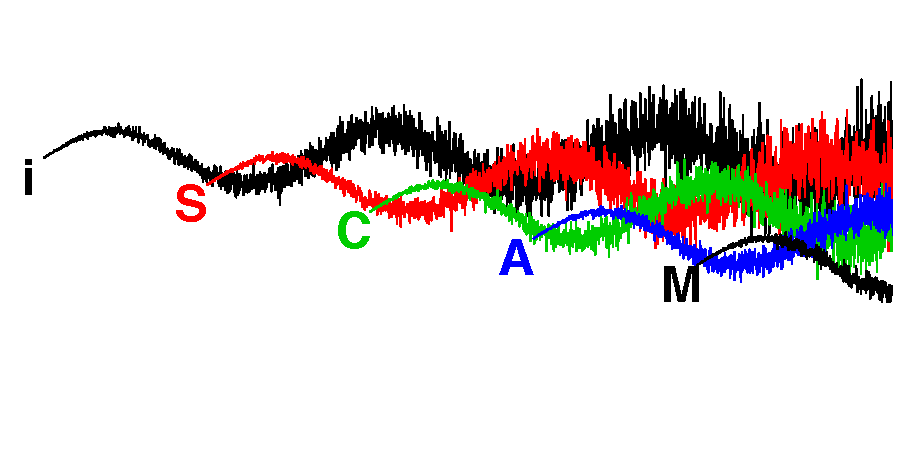
\includegraphics[height=0.6cm]{iScamLogo.pdf}}
%
\title[2011 BC Herring Assessment]{Part I: Moving towards a sustainable fisheries framework for BC herring: data, models \& alternative assumptions.\\
\vfill
Part II: Stock assessment and management advice for BC Herring stocks (2011/2012)\\}
\author{Steven Martell, Jake Schweigert, Jaclyn Cleary, Vivian Haist}
\institute[UBC]
{
University of British Columbia \\
\medskip
{\emph{martell.steve@gmail.com}}
}
\date{\today}
% \today will show current date. 
% Alternatively, you can specify a date.
%
\begin{document}
	\def\newblock{\hskip .11em plus .33em minus .07em}
%
\begin{frame}
\titlepage
\end{frame}
%



%!TEX root = /Users/stevenmartell/Documents/CURRENT PROJECTS/iSCAM-trunk/fba/BC-herring-2011/PRESENTATION/BC-Herring-2011.tex
%%%   %%%   %%%   %%%   %%%   %%%   %%%   %%%   %%%   %%%   %%%   %%%   %%%   %%%   
%% Outline for Part I
%% Introduction:
%% Analytical approach:
%% 
%%%   %%%   %%%   %%%   %%%   %%%   %%%   %%%   %%%   %%%   %%%   %%%   %%%   %%%   
%%%%%%%%%%%%%%%%%%%%%%%%%%%%%%%%%%%%%%%%%%%%%%%%%%%%%
%%%%%%%%%%%%%%%%%%%%%%%%%%%%%%%%%%%%%%%%%%%%%%%%%%%%%
\begin{frame} % (fold)
	\frametitle{Moving towards the sustainable fisheries framework.} 
	\begin{block}
		{Overview} 
		\begin{itemize}
			\item Review of the HCAM model in June 17-18, 2010. 
			\begin{itemize}
				\item Model parameterization of $q$. 
				\item Parametrization of $q$, $M$, and selectivity is confounded. 
			\end{itemize}
			\item Development of a new integrated Statistical Catch Age Model (\iscam). 
			\item Data, assumptions and Analytical methods. 
			\item Outstanding issues. 
		\end{itemize}
	\end{block}
\end{frame}




%%%%%%%%%%%%%%%%%%%%%%%%%%%%%%%%%%%%%%%%%%%%%%%%%%%%%
%%%%%%%%%%%%%%%%%%%%%%%%%%%%%%%%%%%%%%%%%%%%%%%%%%%%%
\section{Introduction} % (fold)
\label{sec:introduction}

%
\begin{frame}
	\frametitle{Introduction} 
	\begin{itemize}
		\item Current harvest control rule for BC herring: 
		\begin{itemize}
			\item Cuttoffs set at 0.25 $B_0$ 
			\item 20\% exploitation rate 
			\item Estimates of $B_0$ were last updated in 1996. 
		\end{itemize}
		\item HCAM model assumed $q=1$ for the dive survey data. 
		\item Natural mortality is modelled as a random-walk. 
		\item Gill net selectivity is a function of weight-at-age. 
	\end{itemize}
\end{frame}

%
\begin{frame}
	\frametitle{Harvest Strategy Compliant with Precautionary Approach} 
	\begin{figure}
		[htbp] \centering 
		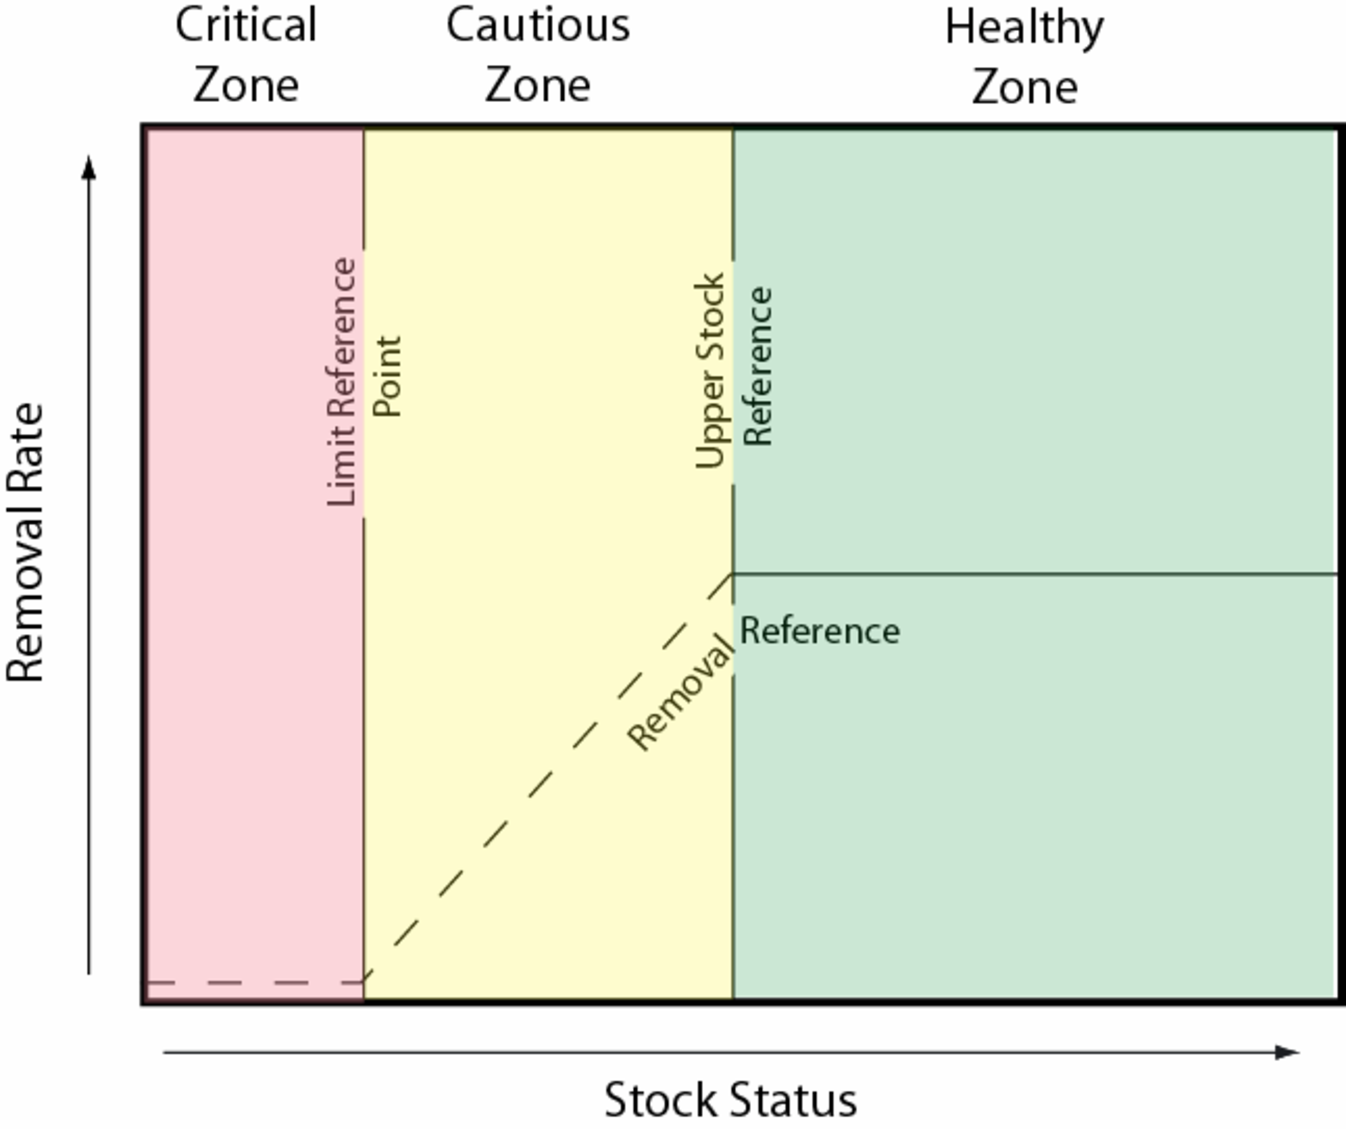
\includegraphics[width=0.7
		\textwidth]{SSF} \caption{Fisheries management framework consistent with a precautionary approach.} \label{fig:label} 
	\end{figure}
\end{frame}

%
\begin{frame}[allowframebreaks]
	\frametitle{Key elements for the new framework} 
	\begin{block}
		{Reference points} 
		\begin{itemize}
			\item Limit Reference Point (LRP) \& Upper Stock Reference (USR) requires knowledge of stock productivity and population scale. 
			\item Removal Rate requires knowledge of stock productivity. 
			\item MSY-based reference points require \textit{a priori} allocation to different gears. 
		\end{itemize}
	\end{block}
	\begin{block}
		{Risk \& Decision making} 
		\begin{itemize}
			\item Onus on being able to reliably determine stock status (informative data). 
		\end{itemize}
	\end{block}
\end{frame}

%
\begin{frame}[allowframebreaks]
	\frametitle{Herring Stock Assessment Model Review} 
	\begin{block}
		{Summary of Panel Recommendations} 
		\begin{itemize}
			\item Panel concluded that $q_2=1$ was inappropriate. 
			\item CUTOFFS can be fixed or annually estimated (should be updated if management objective is 25\% $B_0$) 
			\item A model based approach to estimating $B_0$ and $B_{MSY}$ is appropriate. 
			\item Recruitment variation should be estimated within the model rather than fixing it at a pre-specified level. 
			\item Issues regarding estimating selectivity vs. availability should be explored (data is limited to estimate availability). 
			\item Science advice should be risk neutral. 
			\item MSE should explore elements of the Sustainable Fisheries Framework (i.e., ensure that $B_t>0.4B_{MSY}$ with 95\% certainty over two generations.) 
			\item ... 
		\end{itemize}
	\end{block}
\end{frame}
% section introdution (end)




%%%%%%%%%%%%%%%%%%%%%%%%%%%%%%%%%%%%%%%%%%%%%%%%%%%%%
%%%%%%%%%%%%%%%%%%%%%%%%%%%%%%%%%%%%%%%%%%%%%%%%%%%%%
\section{inputdata} % (fold)
\label{sec:inputdata}

%
\begin{frame}
	{Input data} The input data for \iscam\ is the same as HCAM: 
	\begin{itemize}
		\item Catch by gear, 
		\item Spawn survey index, 
		\item Age-composition data for all gears, 
		\item Empirical weight-at-age data. 
	\end{itemize}
\end{frame}

% section inputdata (end)




%%%%%%%%%%%%%%%%%%%%%%%%%%%%%%%%%%%%%%%%%%%%%%%%%%%%%
%%%%%%%%%%%%%%%%%%%%%%%%%%%%%%%%%%%%%%%%%%%%%%%%%%%%%
\section{analyticalMethods} % (fold)
\label{sec:analyticalmethods}
%
\begin{frame} {Analytical methods} 
	
	\begin{block}
		{Integrated Statistical Catch Age Model (\iscam)}
		\begin{itemize}
			\item The model is based on a statistical catch-age framework first developed by \cite{fournier1982general}.
			
			\item Flexible options for modelling selectivity, natural mortality, \& survey catchability.
			
			\item Integrated framework: joint estimation of policy parameters (e.g., reference pionts).
			\item Bayesian implementation... 
		\end{itemize}
	\end{block}
\end{frame}
%
\begin{frame}[t,allowframebreaks]\frametitle{Assumptions}
	\begin{block}
		{Error distributions}
		\begin{itemize}
			\item Observation errors in catch are lognormal \& $\sigma$ is known.
			\item Errors in spawn survey are lognormal \& $\sigma$ is unknown.
			\item Recruitment deviations are lognormal \& $\sigma$ is unknown.
			\item Age-composition residuals follow a multivariate-logistic distribution.
		\end{itemize}
	\end{block}
	
	\begin{block}
		{Selectivity}
		\begin{itemize}
			\item Seine gears: asymptotic and time invariant.
			\item Gillnet gear: parametric logistic function with weight anomalies as a covariate. 
		\end{itemize}
	\end{block}
	
	\framebreak
	\begin{block}
		{Structural assumptions}
		\begin{itemize}
			\item Age-2 recruitment with a Beverton-Holt model.
			\item Fishing \& natural mortality occur simultaneously (Baranov catch equation).
			\item Natural mortality is age-independent.
			\item Natural mortality can vary over time (random walk, $\sigma=0.1$).
			\item 100\% of the total mortality occurs before spawning.
			\item Fecundity is proportional to mature biomass.
		\end{itemize}
	\end{block}
	
	\begin{block}
		{Equilibrium \& MSY-based reference points}
		\begin{itemize}
			\item $B_o$ is based on average $M$ and average fecundity-at-age.
			\item $B_{MSY}$ is based on average ($M$) and \underline{fecundity in terminal year}.
		\end{itemize}
	\end{block}
	
\end{frame}

\begin{frame}[t,allowframebreaks]\frametitle{Objective function}
	\begin{block}
		{Major components of the objective function}
		\begin{itemize}
			\item Likelihoods for data.
			\item Likelihoods for structural assumptions.
			\item Phased penalties to ensure regular solution.
			\item Prior densities for model parameters.
		\end{itemize}
	\end{block}
	\framebreak
	
	\begin{block}	
		{Likelihoods for data}
		\begin{itemize}
			\item Normal density functions for:
			\begin{itemize}
				\item catch residuals (log-scale) with fixed $\sigma^2$,
				\item spawn survey residuals (log-scale) with estimated $\sigma^2$. 
			\end{itemize}
			\item Multivariate logistic function for age-composition evaluated at the conditional MLE of $\sigma^2$.
		\end{itemize}
	\end{block}
\end{frame}

% section analyticalmethods (end)


%!TEX root = /Users/stevenmartell/Documents/CURRENT PROJECTS/iSCAM-trunk/fba/BC-herring-2011/PRESENTATION/BC-Herring-2011.tex

\section{Part II} % (fold)
\label{sec:part_ii}

\subsection{Introduction} % (fold)
\label{sub:introduction}
%
\begin{frame}[t]\frametitle{Introduction}
	Objectives:
	\begin{enumerate}
		\item Data used in the 2011 assessment.
		\item Overview of the analytical methods.
		\item Present the 2011 stock assessment.
		\item Describe \& present the catch forecasts for 2012.
	\end{enumerate}
\end{frame}

%% subsection introduction (end)

\subsection{2011 Data} % (fold)
\label{sub:2011_data}
%
\begin{frame}[c]\frametitle{Data used in the 2011 stock assessment}
	\begin{itemize}
		\item Catch by gear type.
		\item Spawn survey data.
		\item Age-composition data.
		\item Empirical weight-at-age data. 
	\end{itemize}
\end{frame}
%
\begin{frame}[t]\frametitle{Catch by gear (1950:2011)}
	\only<1>{
	\begin{figure}[htbp]
		\centering
		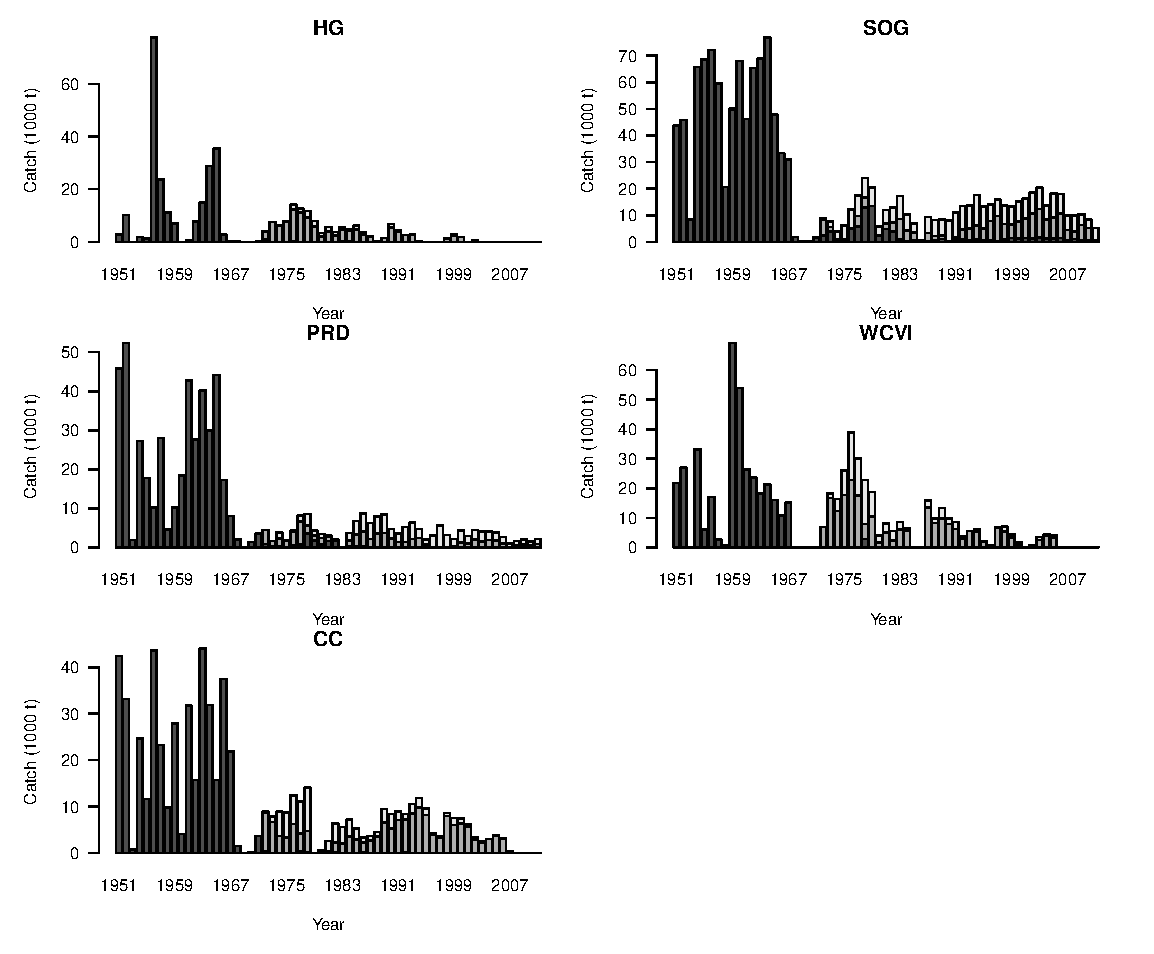
\includegraphics[clip,trim=0 304 300 0 ]
		{../FIGS/iscam_fig_CatchMajorAreas}
		\caption{Catch by gear for Haida Gwaii.}
	\end{figure}
	}
	\only<2>{
	\begin{figure}[htbp]
		\centering
		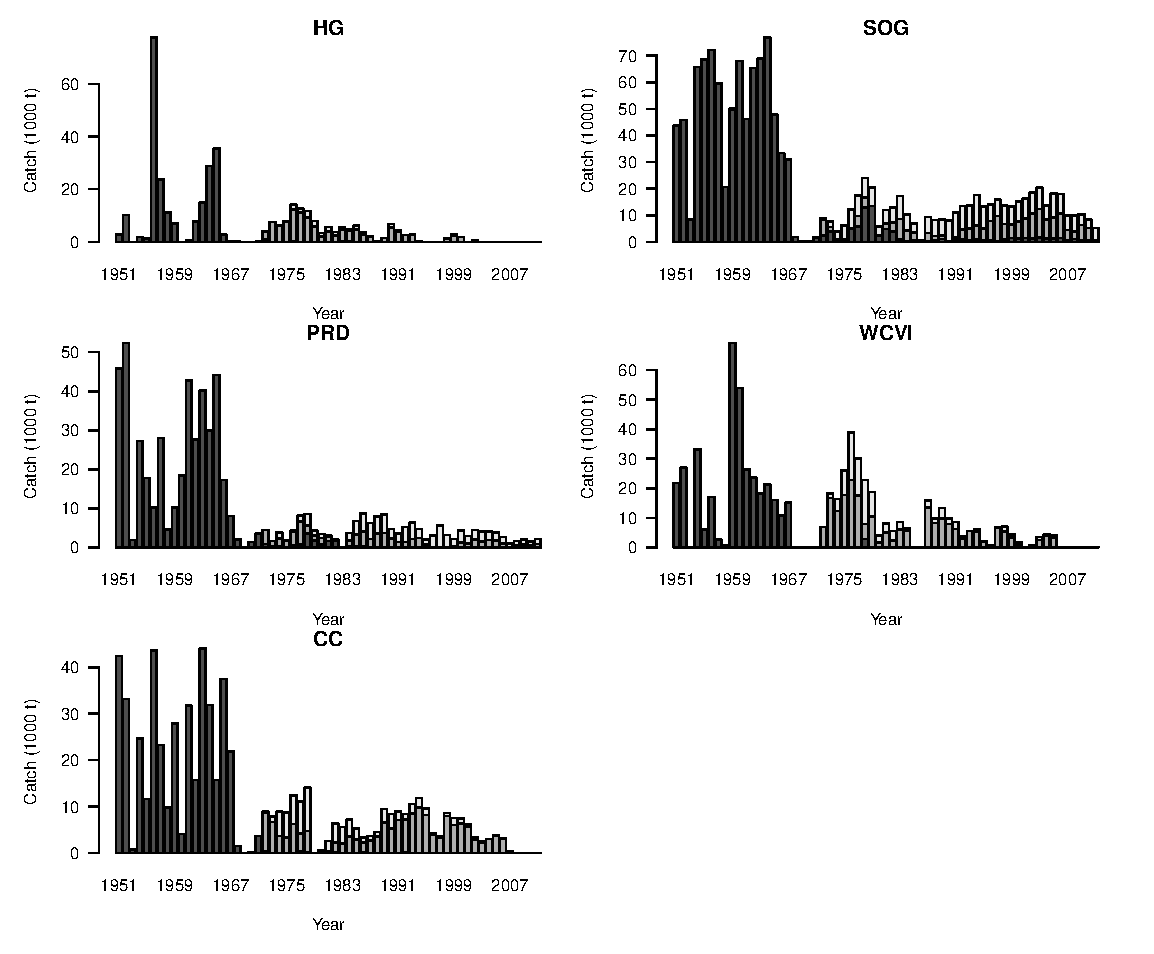
\includegraphics[clip,trim=0 156 300 155 ]
		{../FIGS/iscam_fig_CatchMajorAreas}
		\caption{Catch by gear for Prince Rupert District.}
	\end{figure}
	}
	\only<3>{
	\begin{figure}[htbp]
		\centering
		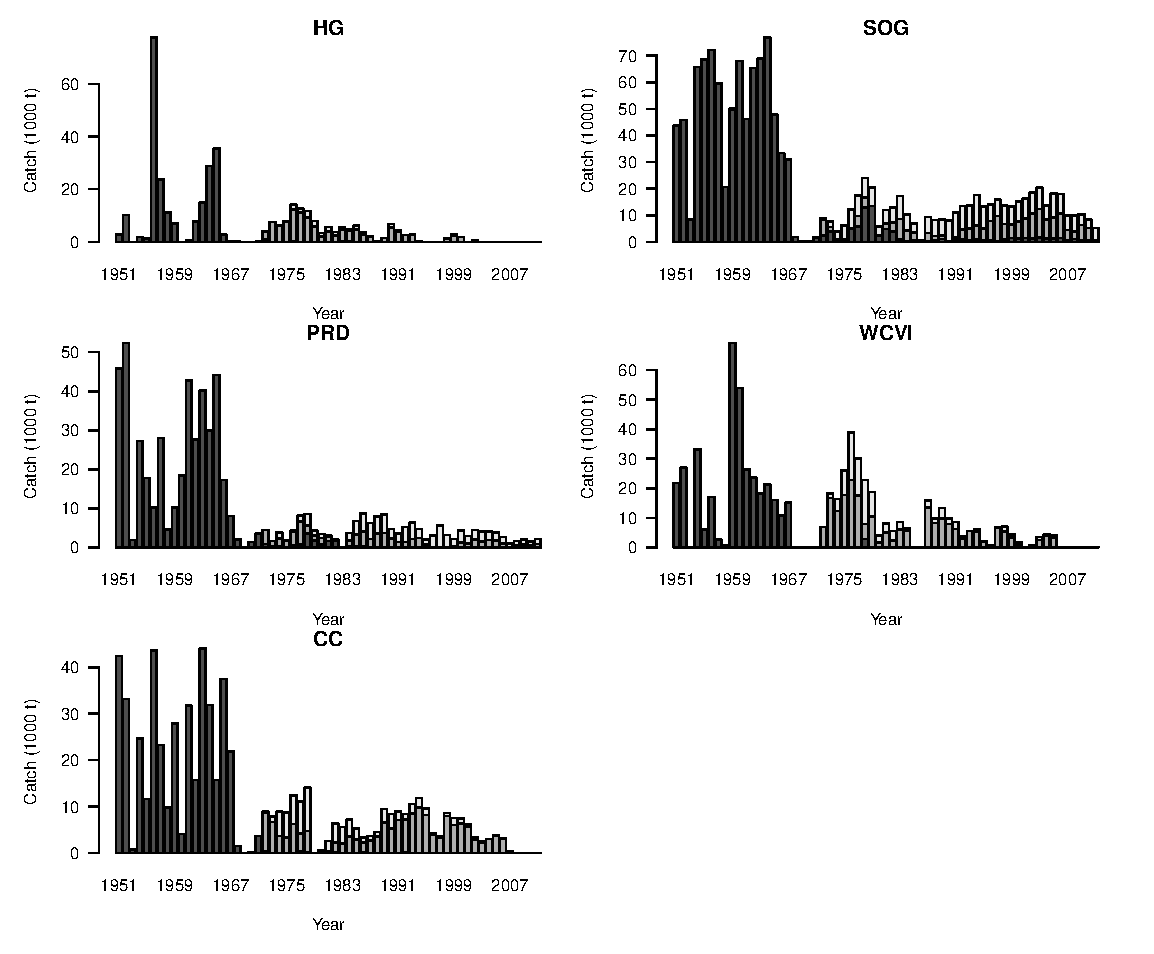
\includegraphics[clip,trim=0 0 300 301 ]
		{../FIGS/iscam_fig_CatchMajorAreas}
		\caption{Catch by gear for Central Coast.}
	\end{figure}
	}
	\only<4>{
	\begin{figure}[htbp]
		\centering
		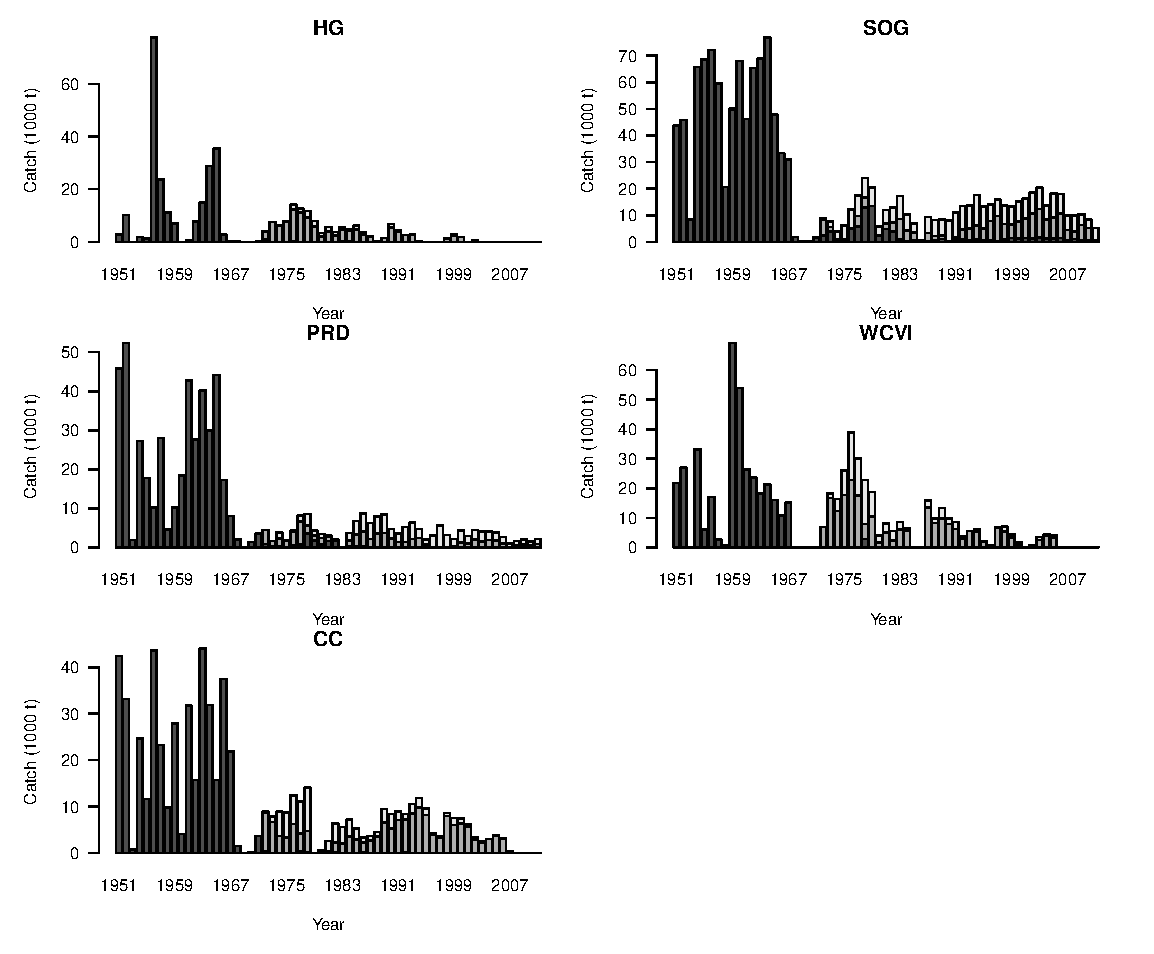
\includegraphics[clip,trim=300 304 0 0 ]
		{../FIGS/iscam_fig_CatchMajorAreas}
		\caption{Catch by gear for Strait of Georgia.}
	\end{figure}
	}
	\only<5>{
	\begin{figure}[htbp]
		\centering
		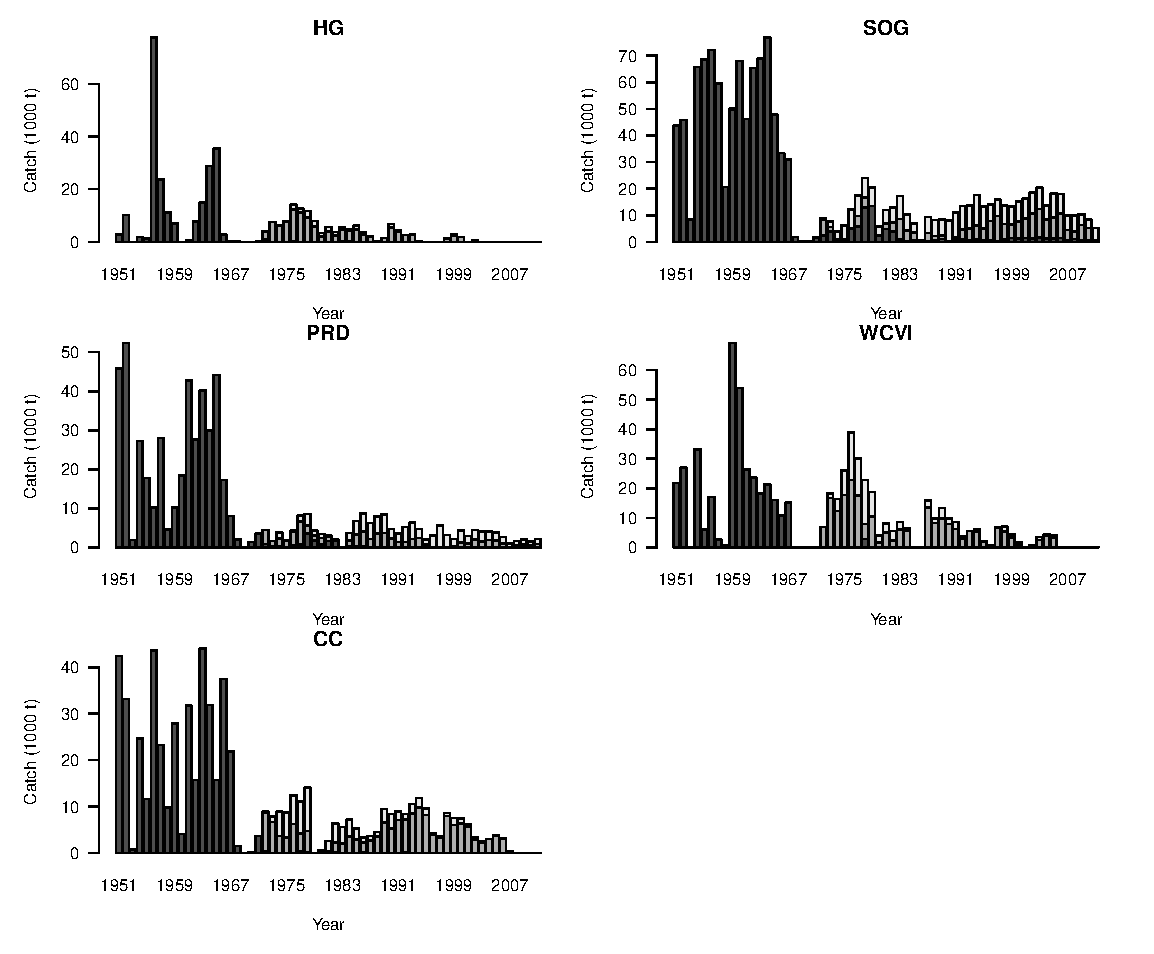
\includegraphics[clip,trim=300 156 0 155 ]
		{../FIGS/iscam_fig_CatchMajorAreas}
		\caption{Catch by gear for West Coast of Vancouver Island.}
	\end{figure}
	}
\end{frame}
%
\begin{frame}[t]\frametitle{Spawning activity in 2010}
	\only<1>{
	\begin{figure}[htbp]
		\centering
		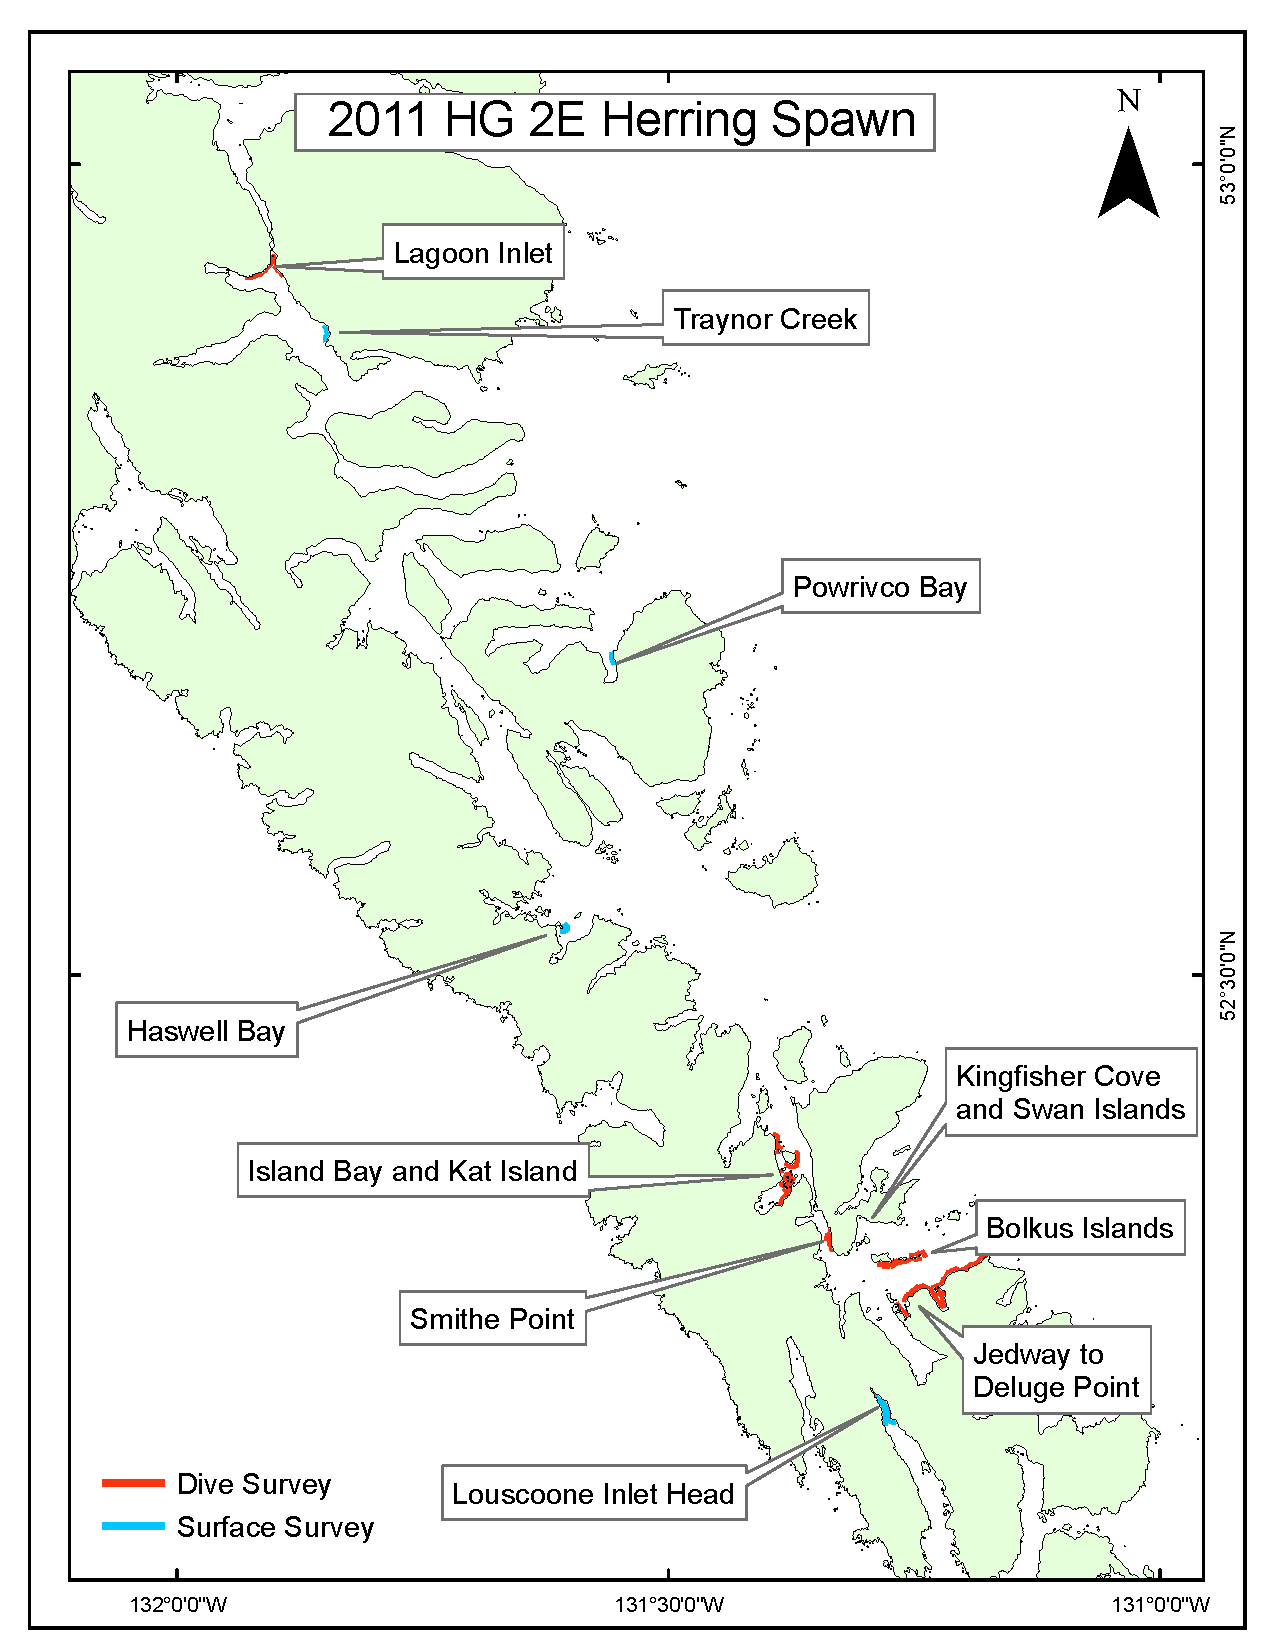
\includegraphics[scale=0.23]
		{../FIGS/PBSfigs/2011_spawn_HG_2E_July13}
		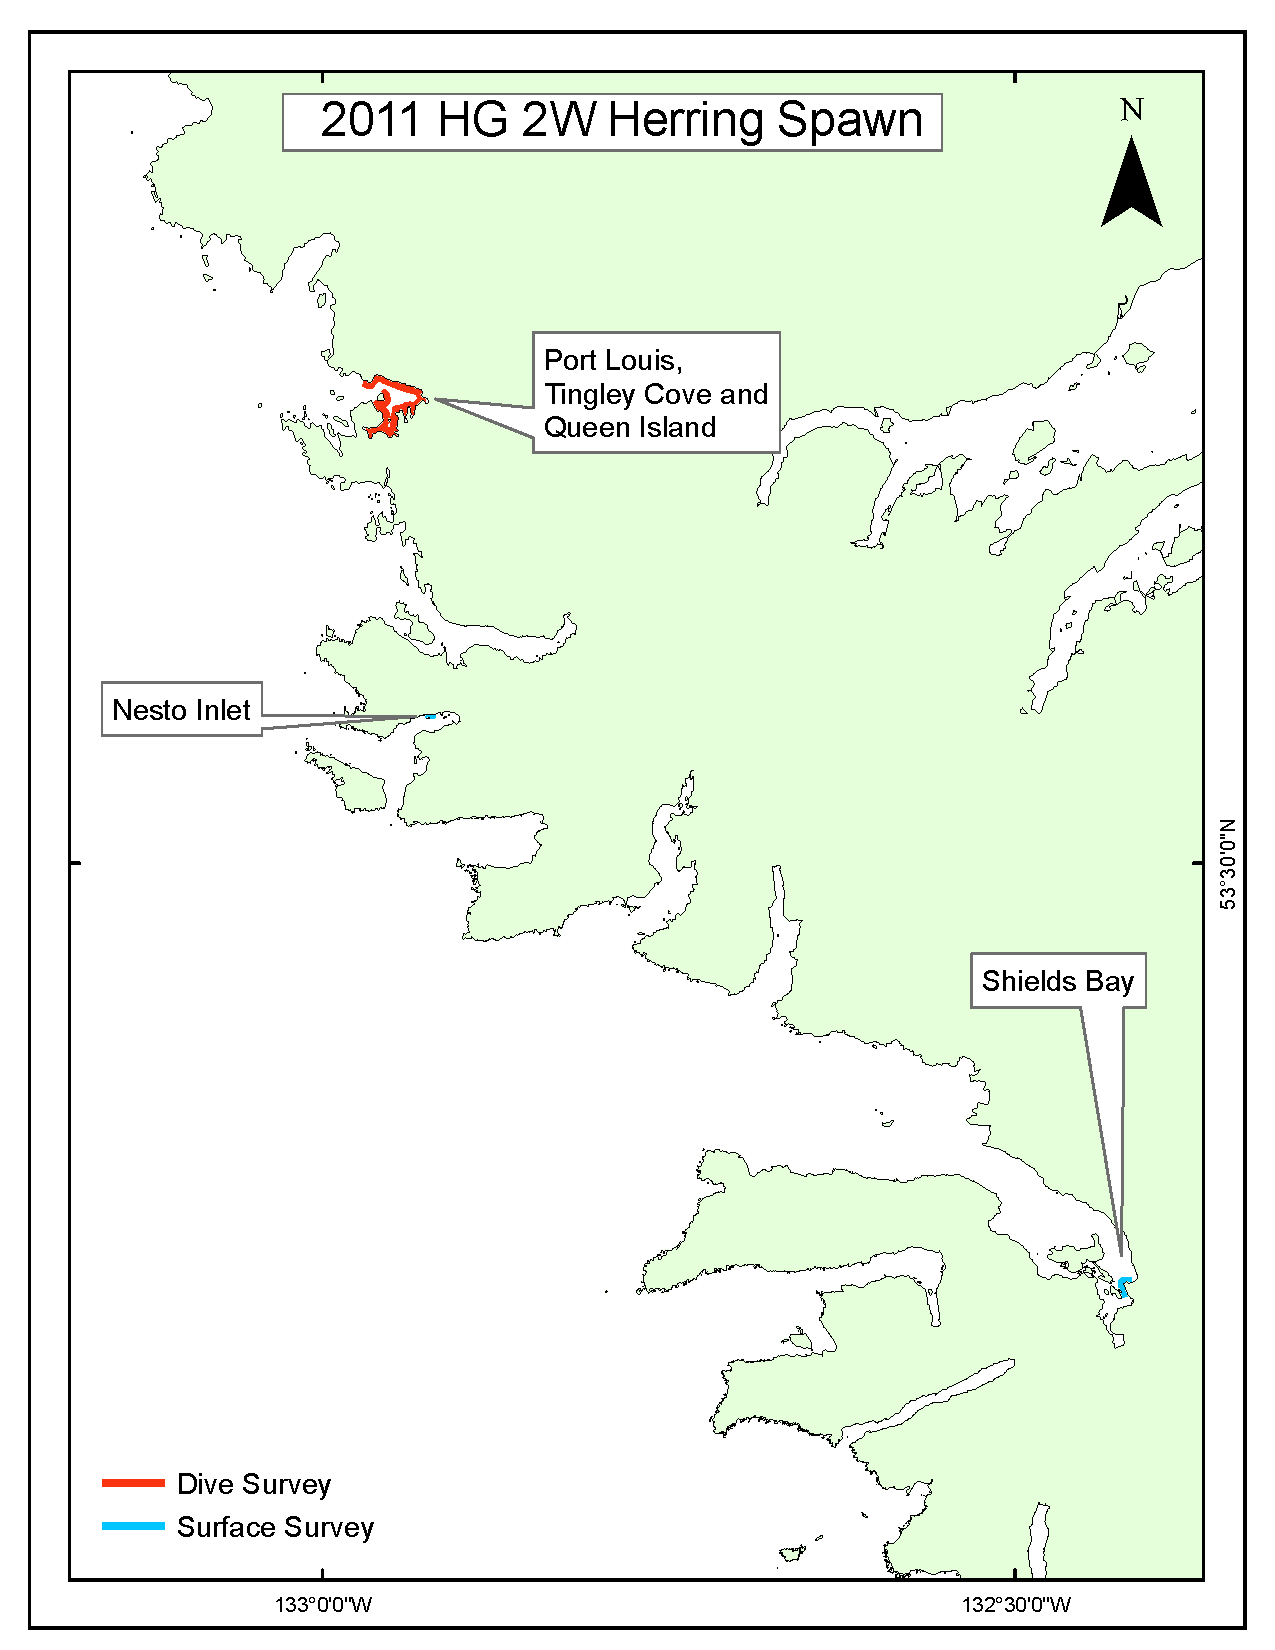
\includegraphics[scale=0.23]
		{../FIGS/PBSfigs/2011_spawn_HG_2W_July13}
		%{../FIGS/PBSfigs/2011-HG-Prelim-WG}
		\caption{2010 Spawning activity in Haida Gwaii.}
	\end{figure}
	}
	\only<2>{
	\begin{figure}[htbp]
		\centering
		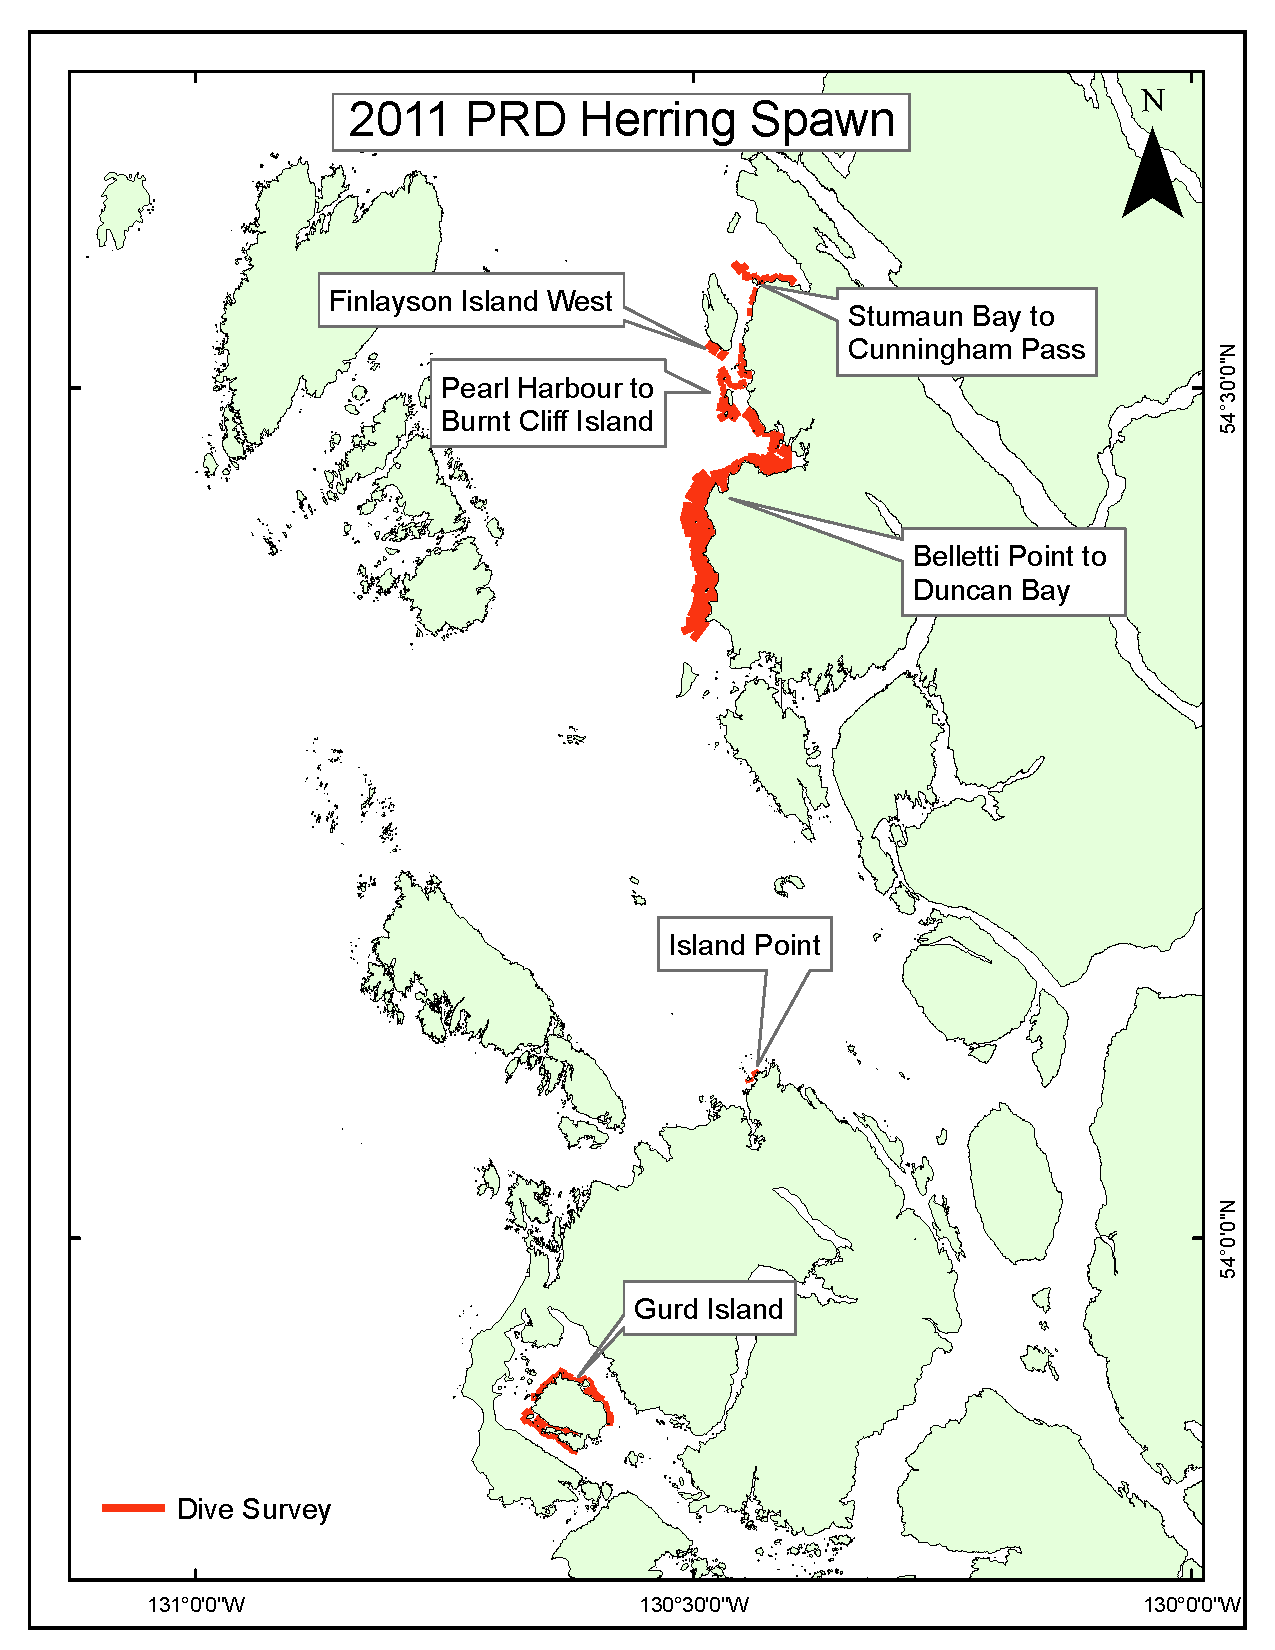
\includegraphics[scale=0.23]
		{../FIGS/PBSfigs/2011_spawn_PRD_July13}
		\caption{2010 Spawning activity in Prince Rupert District.}
	\end{figure}
	}
	\only<3>{
	\begin{figure}[htbp]
		\centering
		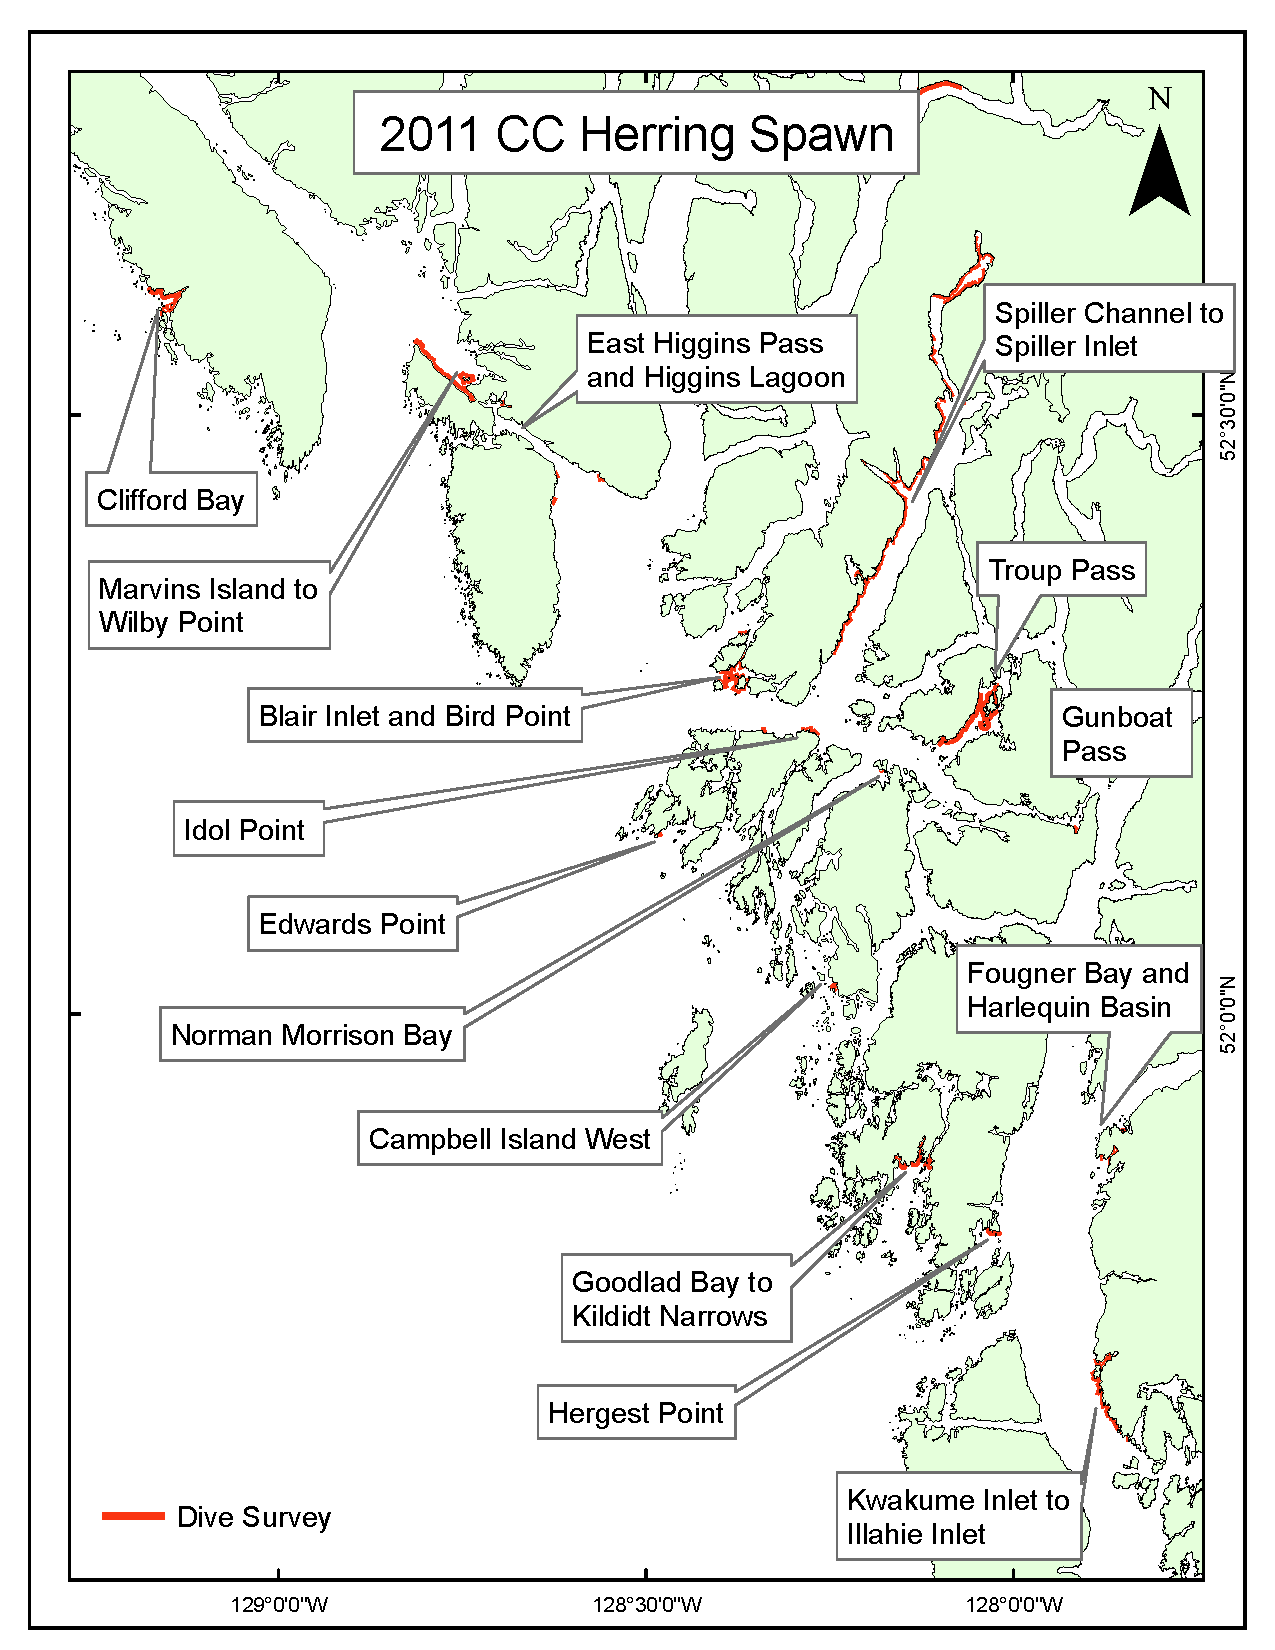
\includegraphics[scale=0.23]
		{../FIGS/PBSfigs/2011_spawn_CCJuly13}
		\caption{2010 Spawning activity in Central Coast.}
	\end{figure}
	}
	\only<4>{
	\begin{figure}[htbp]
		\centering
		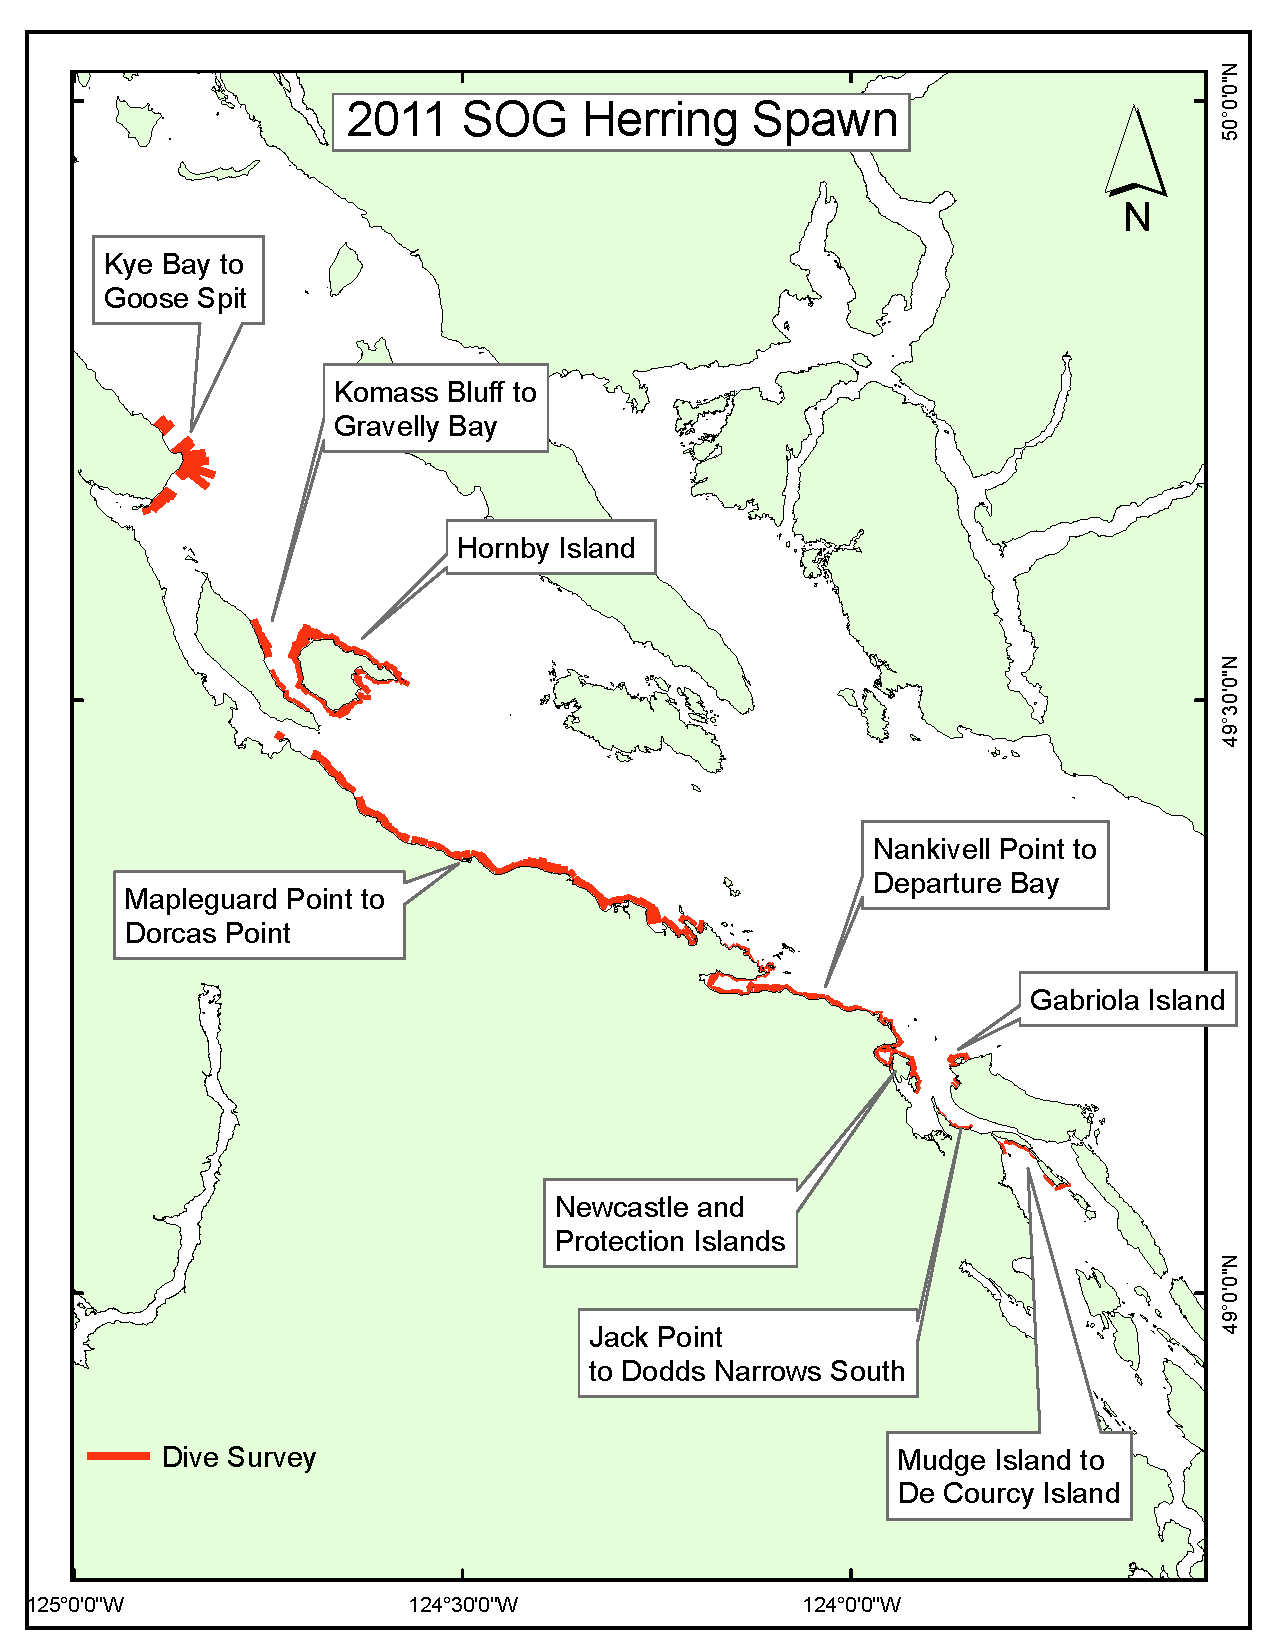
\includegraphics[scale=0.23]
		{../FIGS/PBSfigs/2011_spawn_SOG_July13}
		\caption{2010 Spawning activity in Strait of Georgia.}
	\end{figure}
	}
	\only<5>{
	\begin{figure}[htbp]
		\centering
		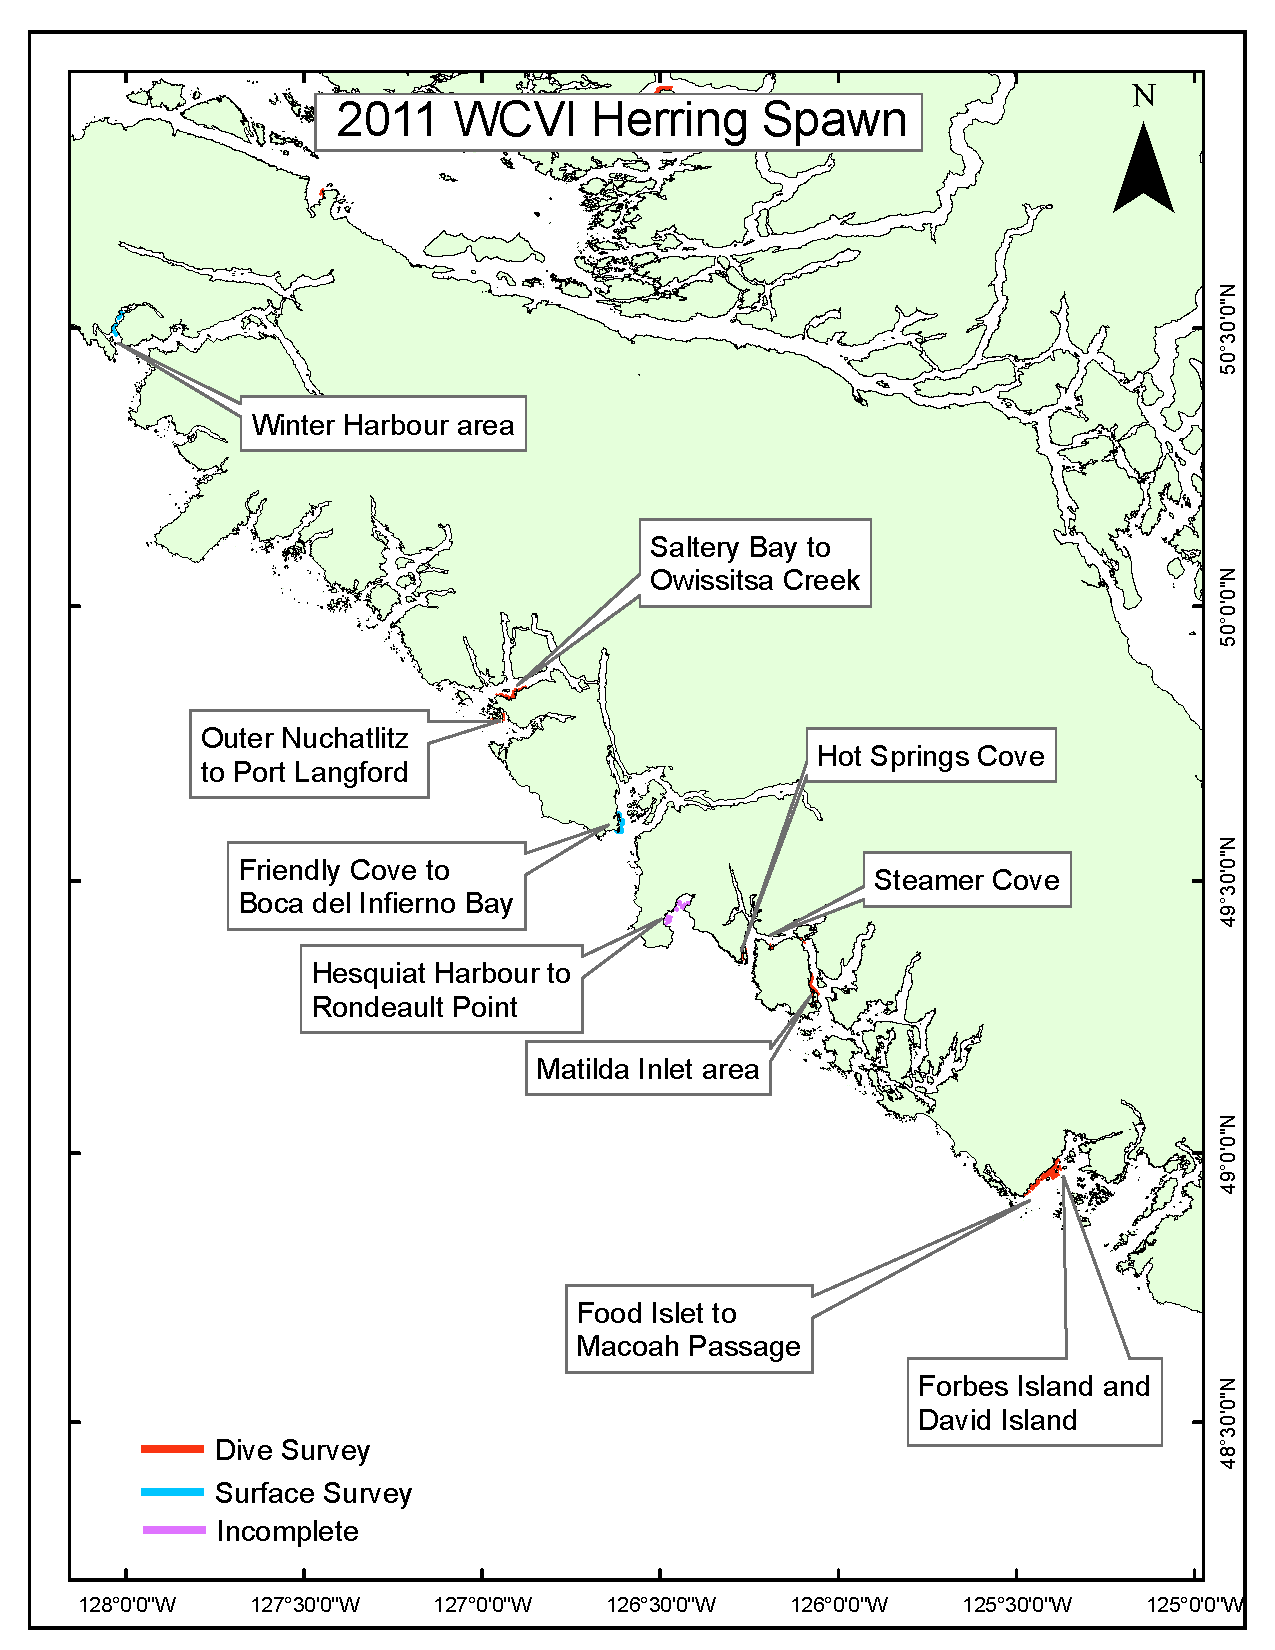
\includegraphics[scale=0.23]
		{../FIGS/PBSfigs/2011_spawn_WCVI_August16}
		\caption{2010 Spawning activity in West Coast Vancouver Island.}
	\end{figure}
	}
\end{frame}
%
\begin{frame}[t]\frametitle{Spawn survey time series}
	\only<1>{
	\begin{figure}[htbp]
		\centering
		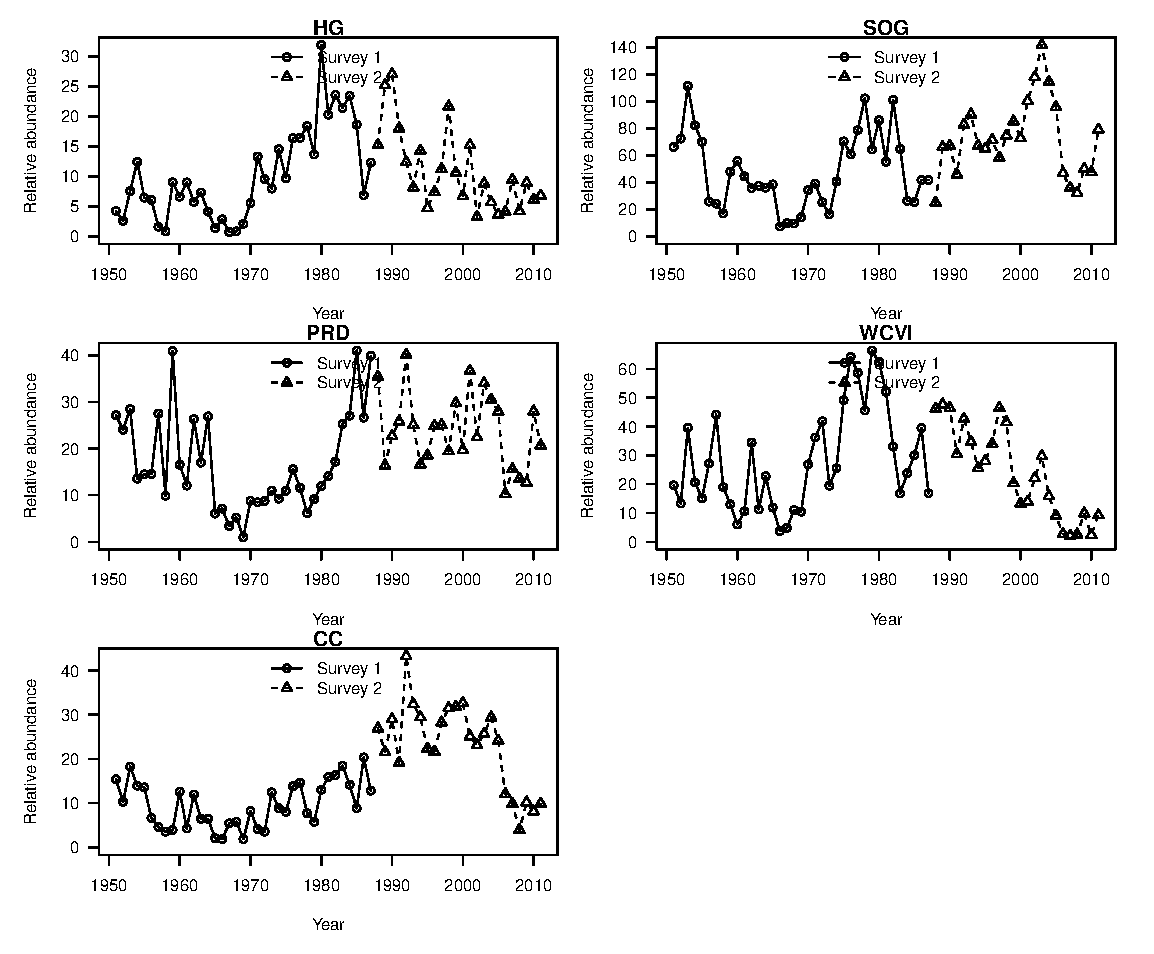
\includegraphics[clip,trim=0 304 275 0]
		{../FIGS/iscam_fig_SurveyMajorAreas}
		\caption{Spawn survey series in Haida Gwaii.}
	\end{figure}
	}
	%
	\only<2>{
	\begin{figure}[htbp]
		\centering
		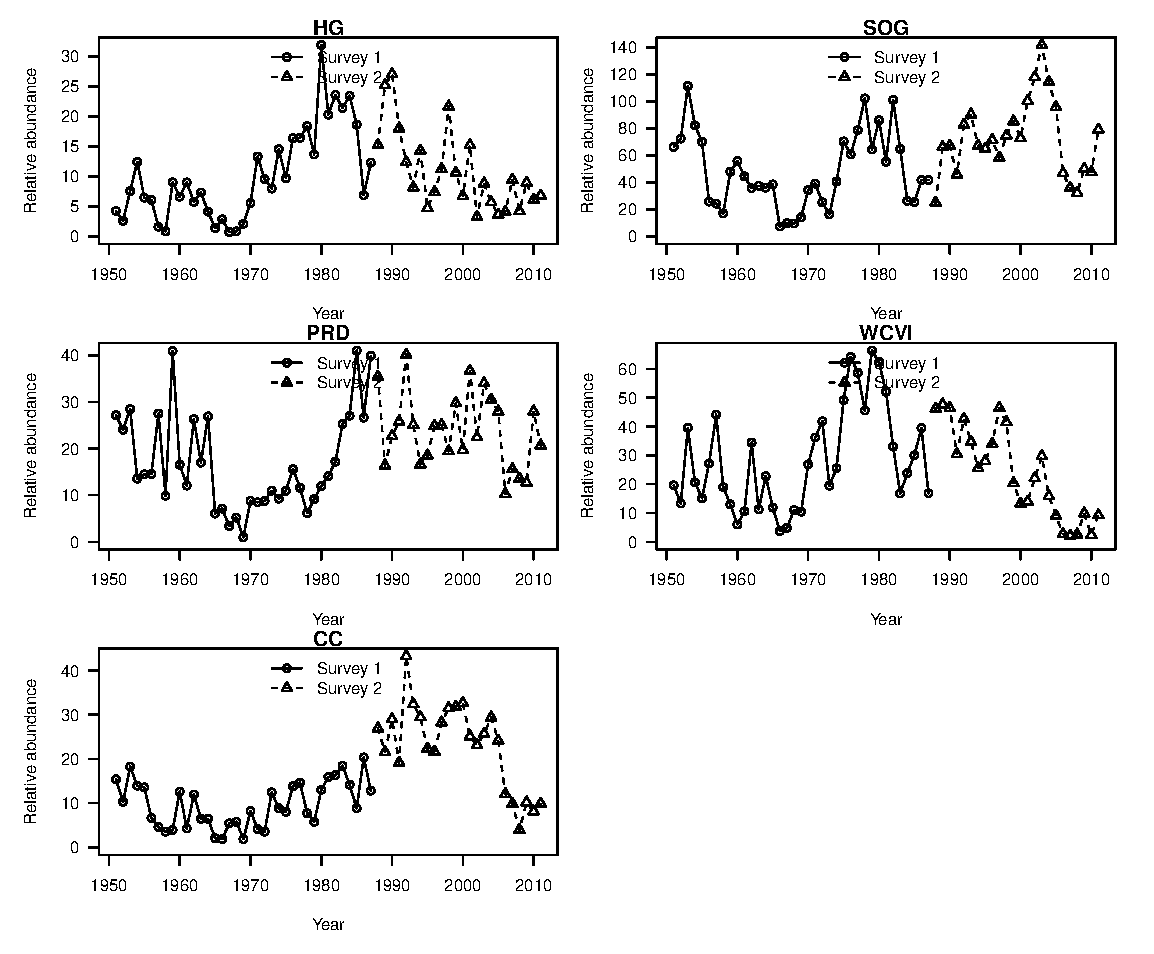
\includegraphics[clip,trim=0 156 275 155]
		{../FIGS/iscam_fig_SurveyMajorAreas}
		\caption{Spawn survey series in Prince Rupert District.}
	\end{figure}
	}
	%
	\only<3>{
	\begin{figure}[htbp]
		\centering
		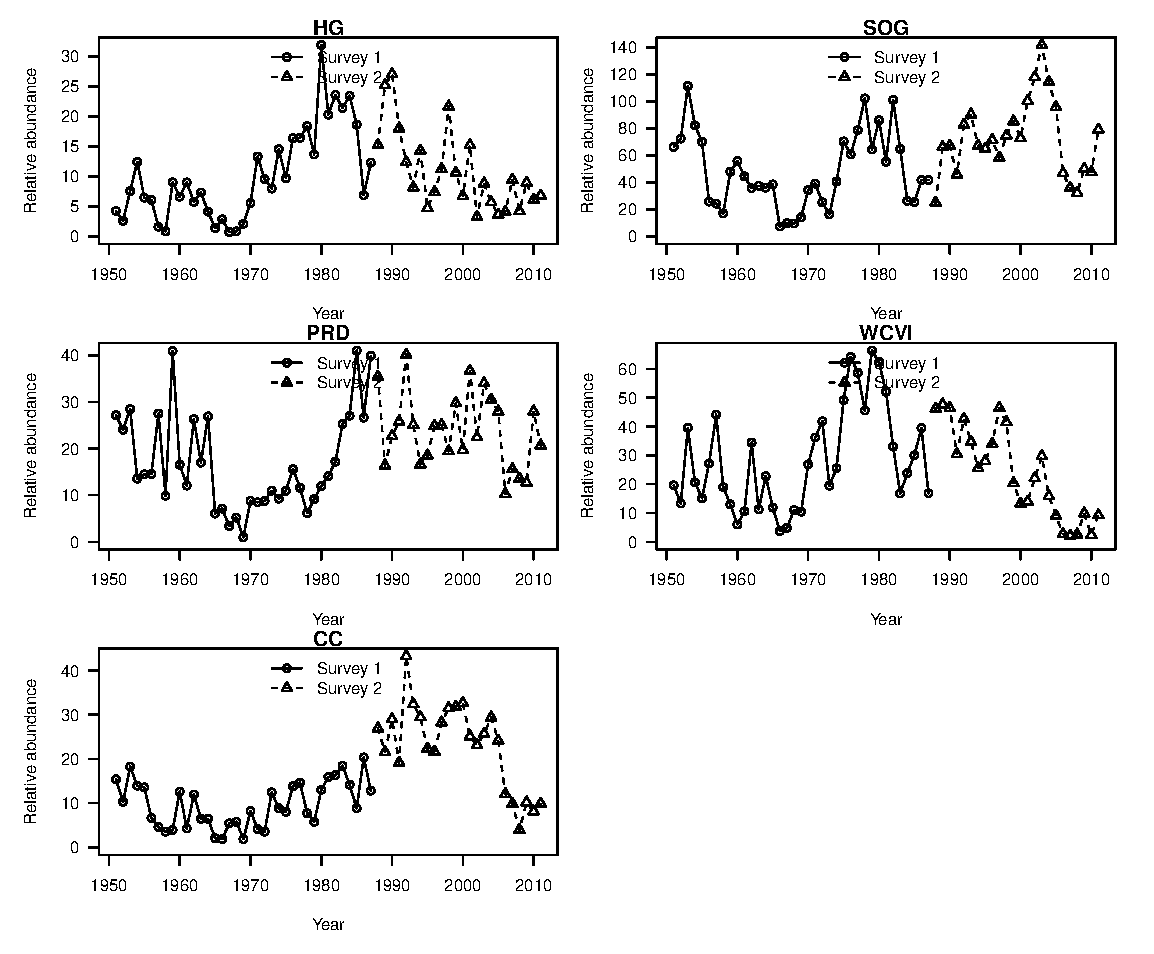
\includegraphics[clip,trim=0 0 275 301]
		{../FIGS/iscam_fig_SurveyMajorAreas}
		\caption{Spawn survey series in Central Coast.}
	\end{figure}
	}
	%
	\only<4>{
	\begin{figure}[htbp]
		\centering
		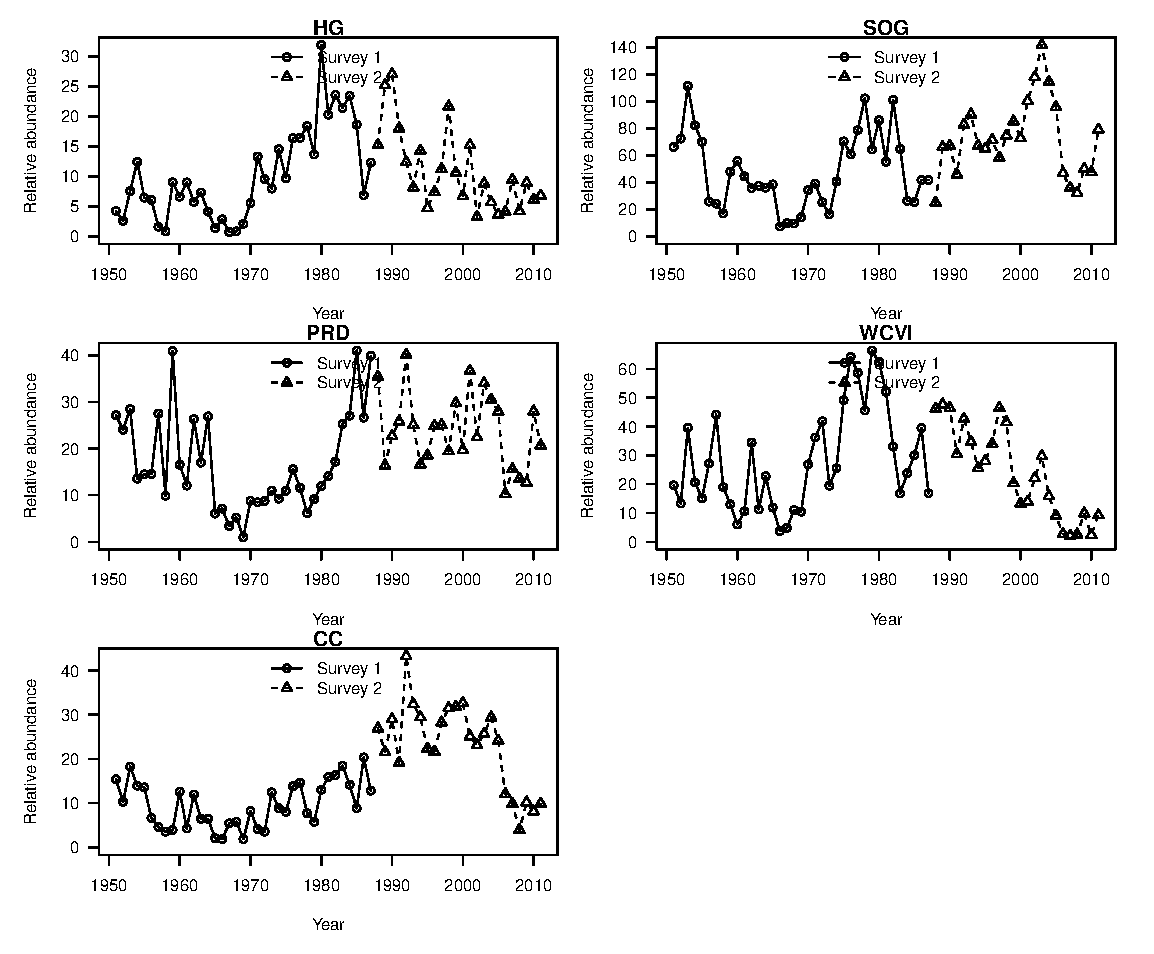
\includegraphics[clip,trim=275 304 0 0]
		{../FIGS/iscam_fig_SurveyMajorAreas}
		\caption{Spawn survey series in Strait of Georgia.}
	\end{figure}
	}
	%
	\only<5>{
	\begin{figure}[htbp]
		\centering
		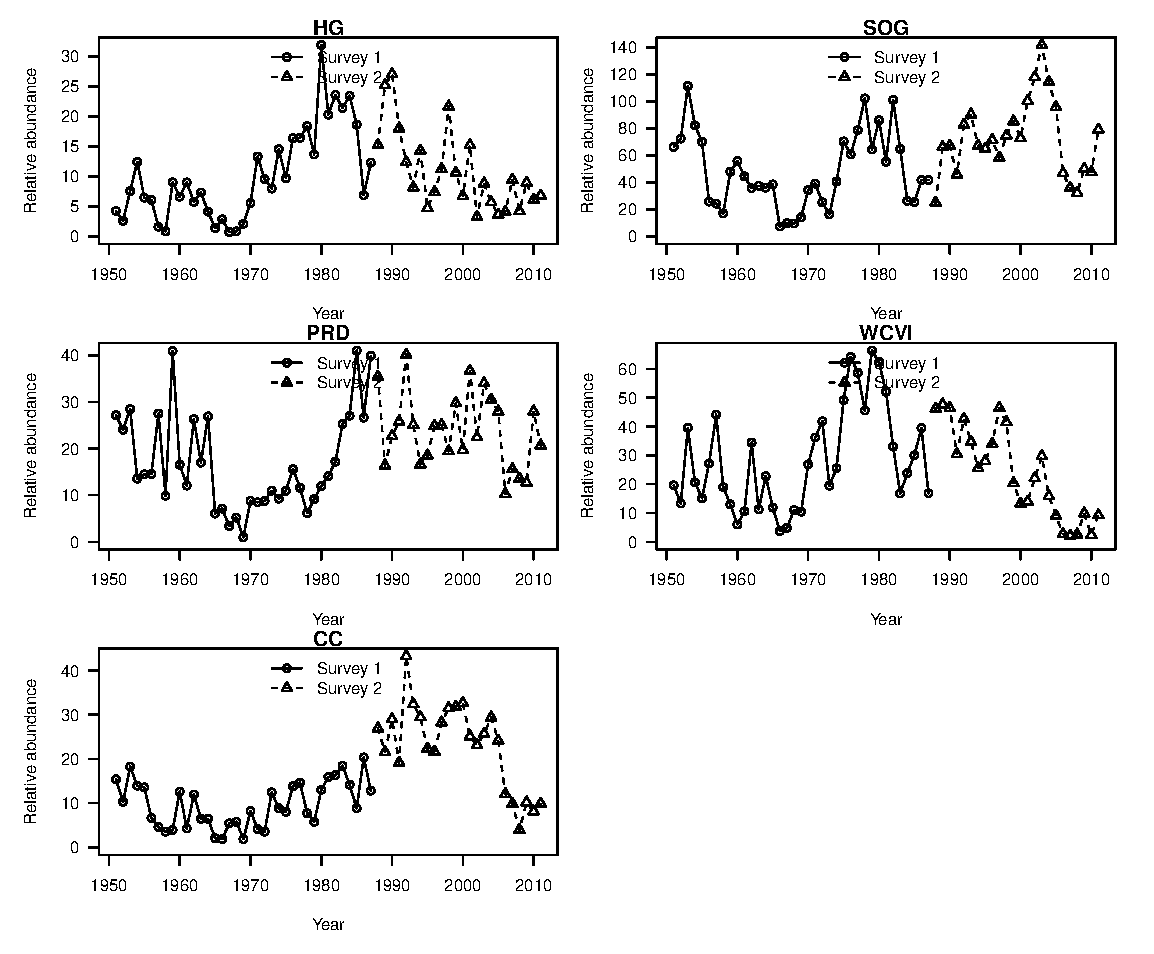
\includegraphics[clip,trim=275 156 0 155]
		{../FIGS/iscam_fig_SurveyMajorAreas}
		\caption{Spawn survey series in West Coast of Vancouver Island.}
	\end{figure}
	}
\end{frame}
%
\begin{frame}[t]\frametitle{Age-composition data}
	\only<1>{
	\begin{figure}[htbp]
		\centering
		\vspace{-0.5cm}	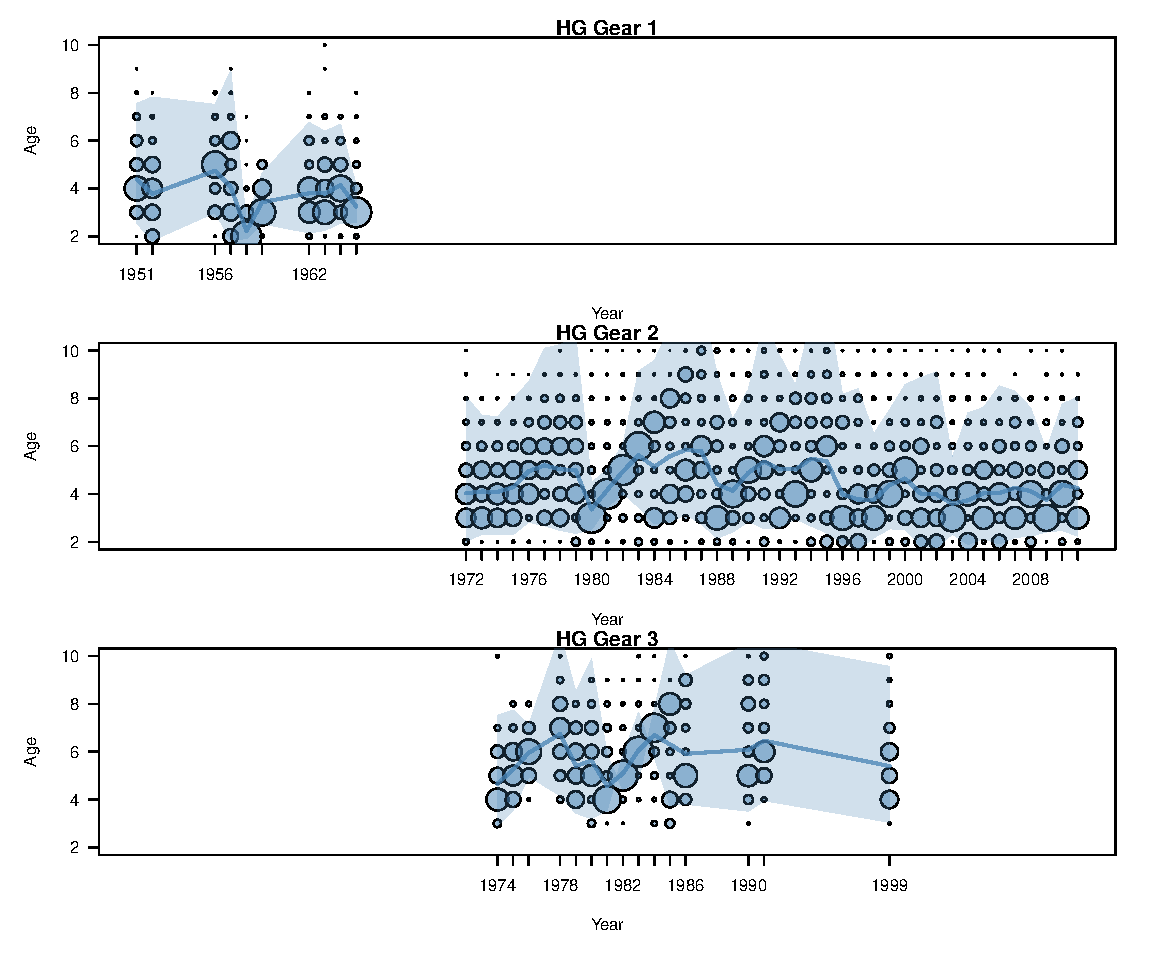
\includegraphics
		[height=0.85\textheight,width=\textwidth]
		{../FIGS/iscam_fig_AgeCompsHG}
		\vspace{-1cm}
		\caption{Haida Gwaii: winter seine, seine-roe, gillnet.}
	\end{figure}
	}
	%
	\only<2>{
	\begin{figure}[htbp]
		\centering
		\vspace{-0.5cm}	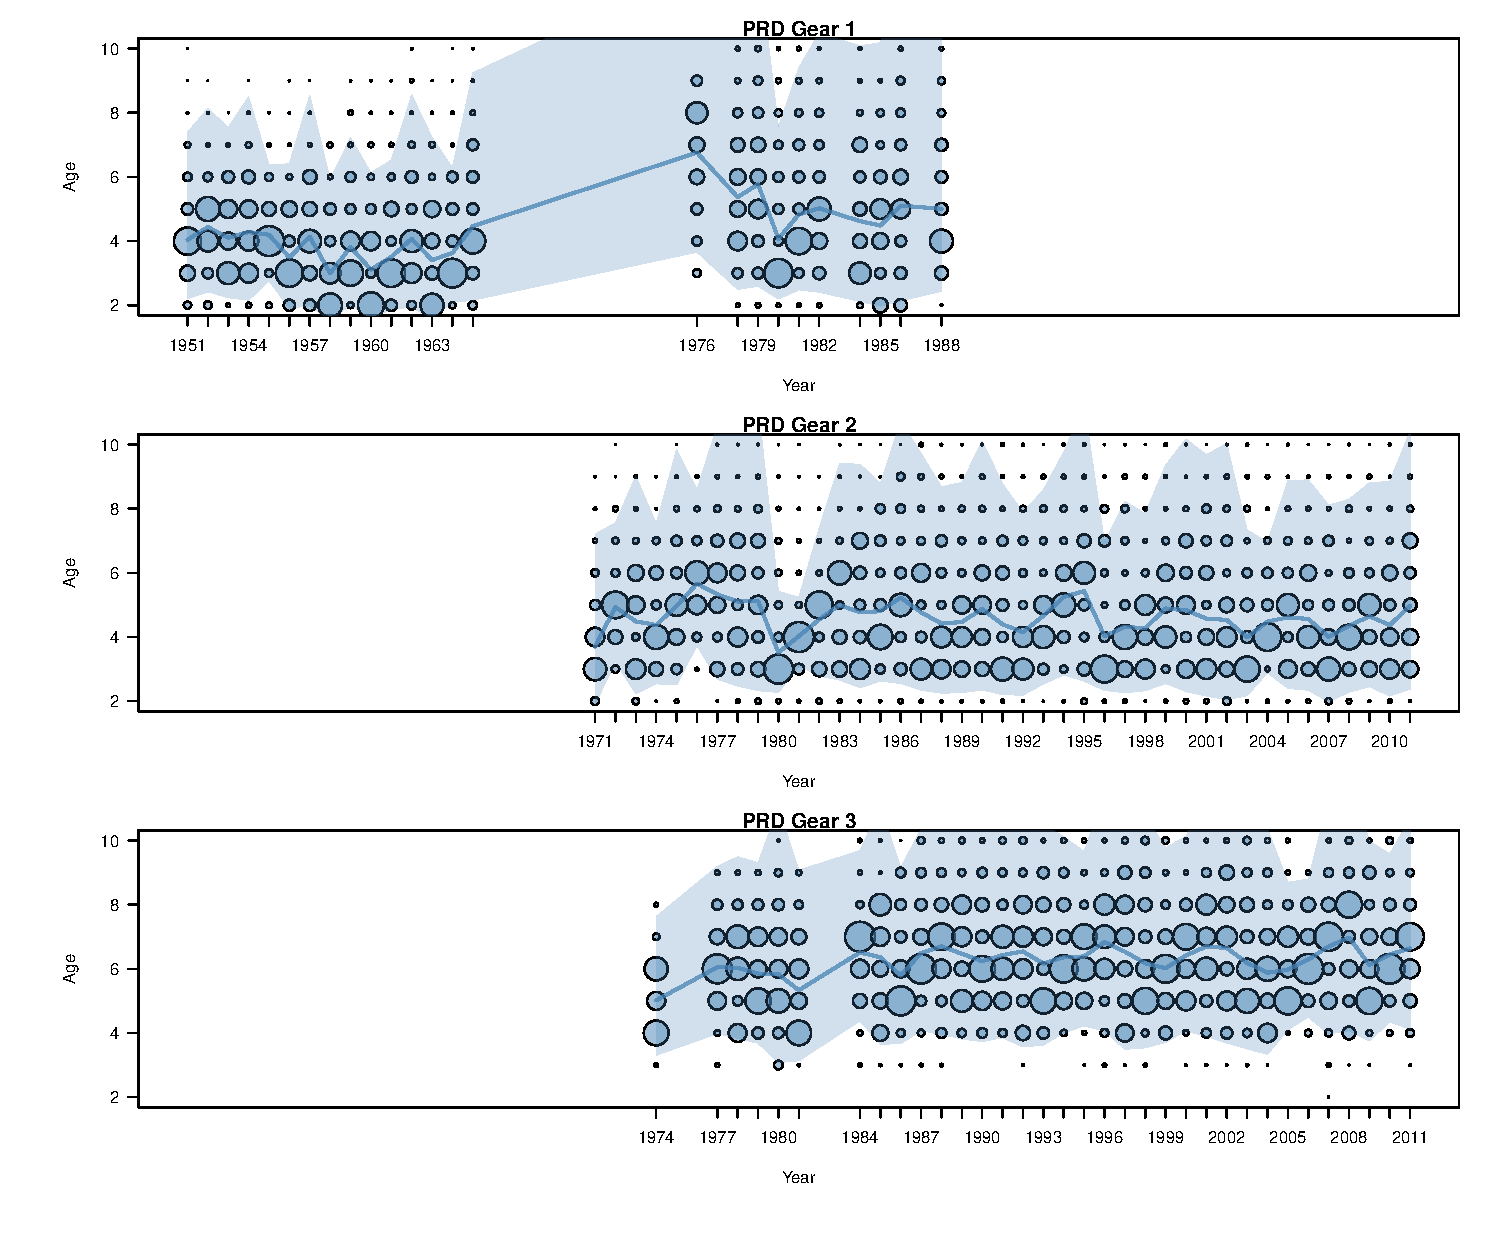
\includegraphics
		[height=0.85\textheight,width=\textwidth]
		{../FIGS/iscam_fig_AgeCompsPRD}
		\vspace{-1cm}
		\caption{Prince Rupert District: winter seine, seine-roe, gillnet.}
	\end{figure}
	}
	%
	\only<3>{
	\begin{figure}[htbp]
		\centering
		\vspace{-0.5cm}	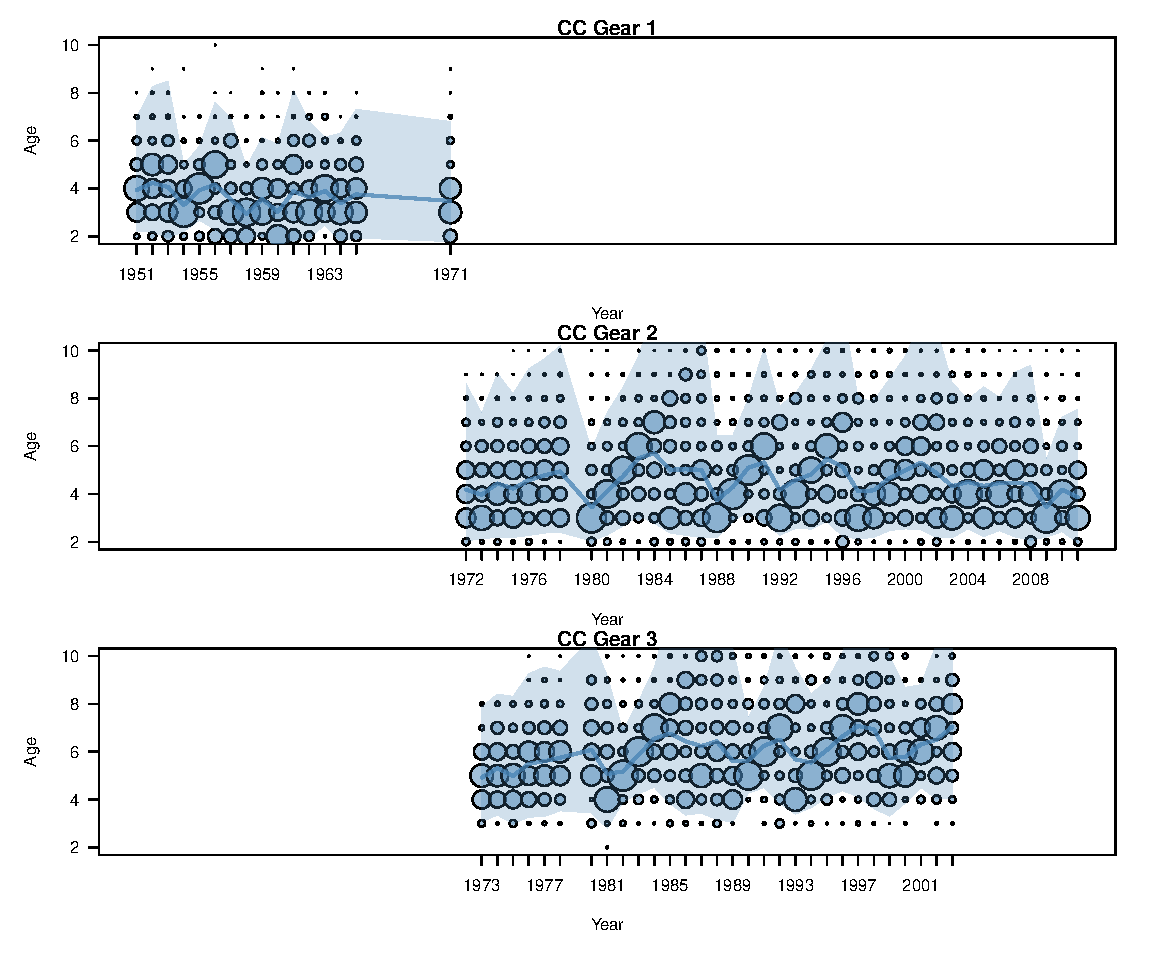
\includegraphics
		[height=0.85\textheight,width=\textwidth]
		{../FIGS/iscam_fig_AgeCompsCC}
		\vspace{-1cm}
		\caption{Central Coast: winter seine, seine-roe, gillnet.}
	\end{figure}
	}
	%
	\only<4>{
	\begin{figure}[htbp]
		\centering
		\vspace{-0.5cm}	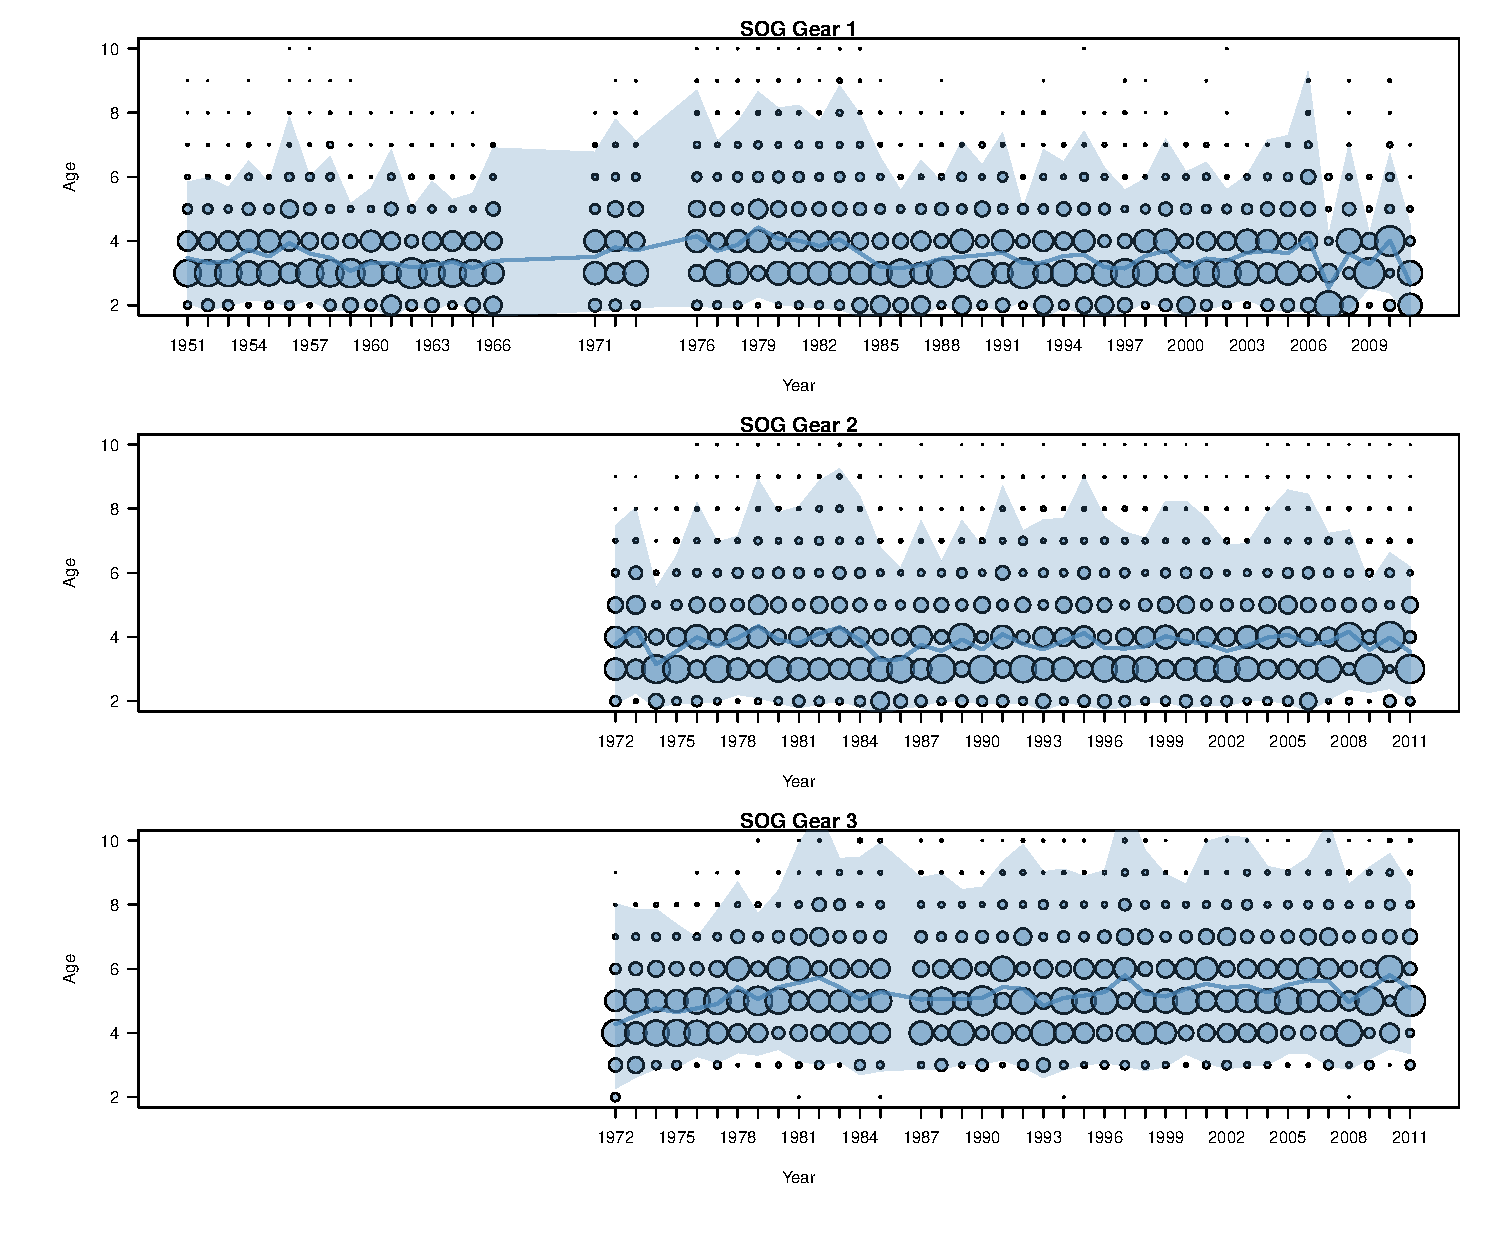
\includegraphics
		[height=0.85\textheight,width=\textwidth]
		{../FIGS/iscam_fig_AgeCompsSOG}
		\vspace{-1cm}
		\caption{Strait of Georgia: winter seine, seine-roe, gillnet.}
	\end{figure}
	}
	%
	\only<5>{
	\begin{figure}[htbp]
		\centering
		\vspace{-0.5cm}	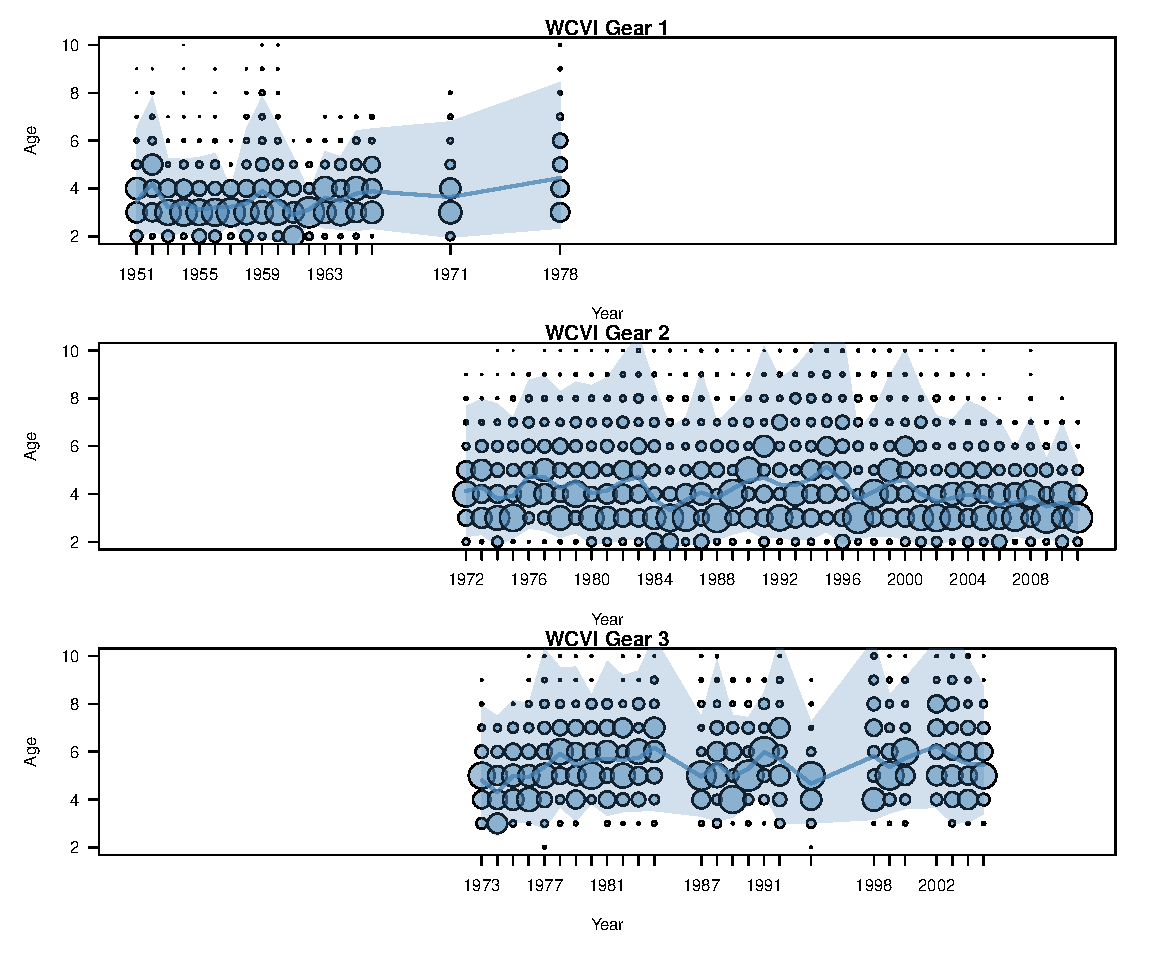
\includegraphics
		[height=0.85\textheight,width=\textwidth]
		{../FIGS/iscam_fig_AgeCompsWCVI}
		\vspace{-1cm}
		\caption{West Coast Vancouver Island: winter seine, seine-roe, gillnet.}
	\end{figure}
	}
	
\end{frame}
%
\begin{frame}[t]\frametitle{Weight-at-age}
	\only<1>{
	\begin{figure}[htbp]
		\centering
		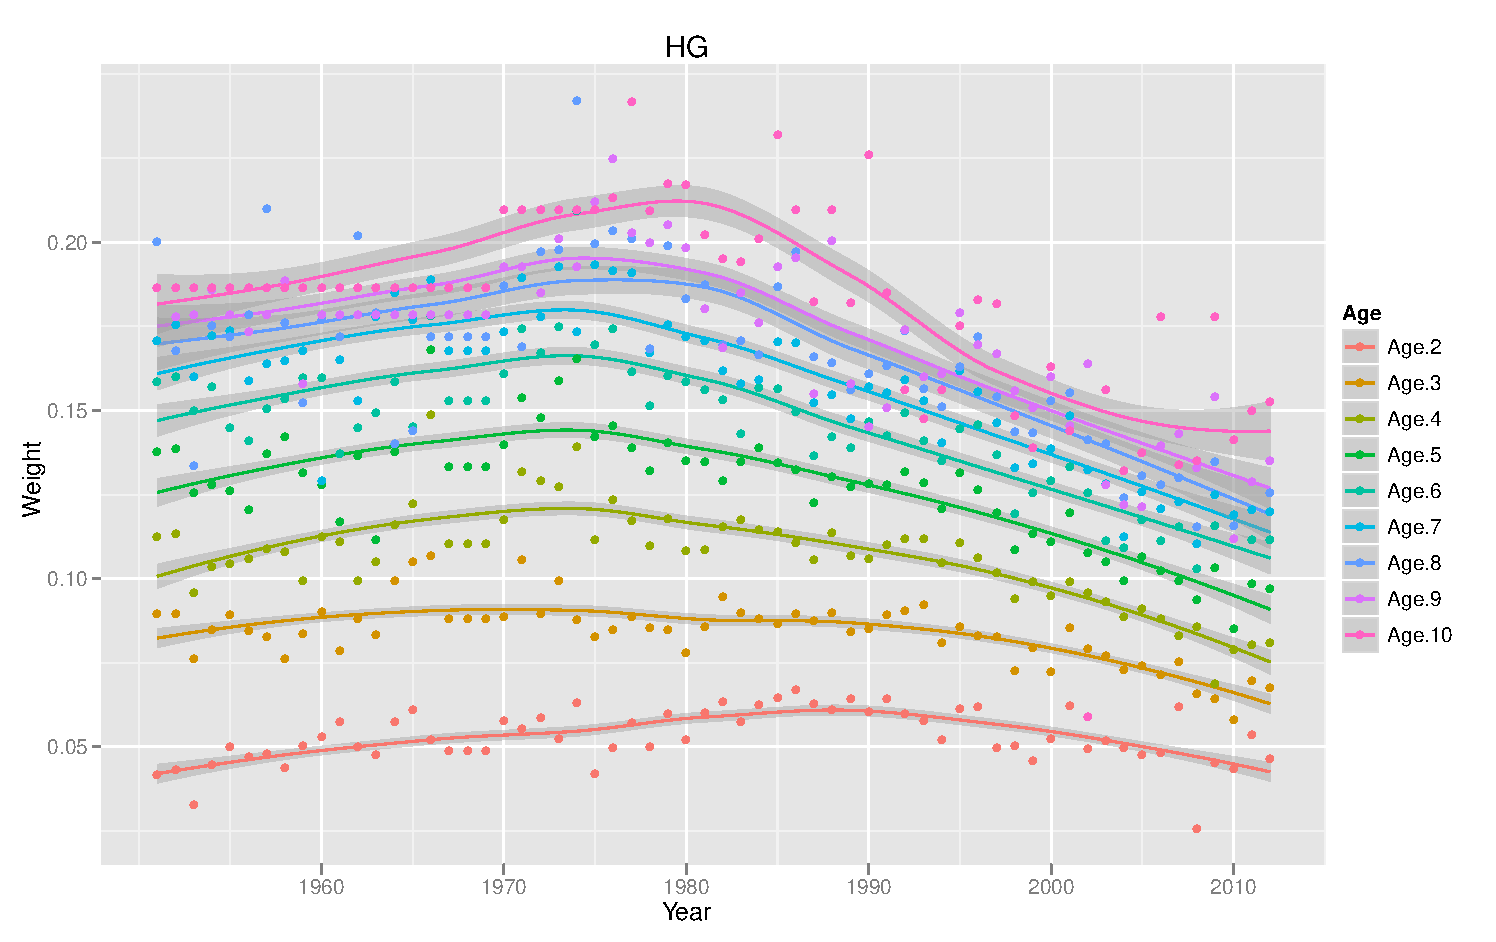
\includegraphics[scale=0.4]
		{../FIGS/iscam_fig_weight-at-age_HG}
		\caption{Haida Gwaii: empirical weight-at-age (kg).}
	\end{figure}
	}
	%
	\only<2>{
	\begin{figure}[htbp]
		\centering
		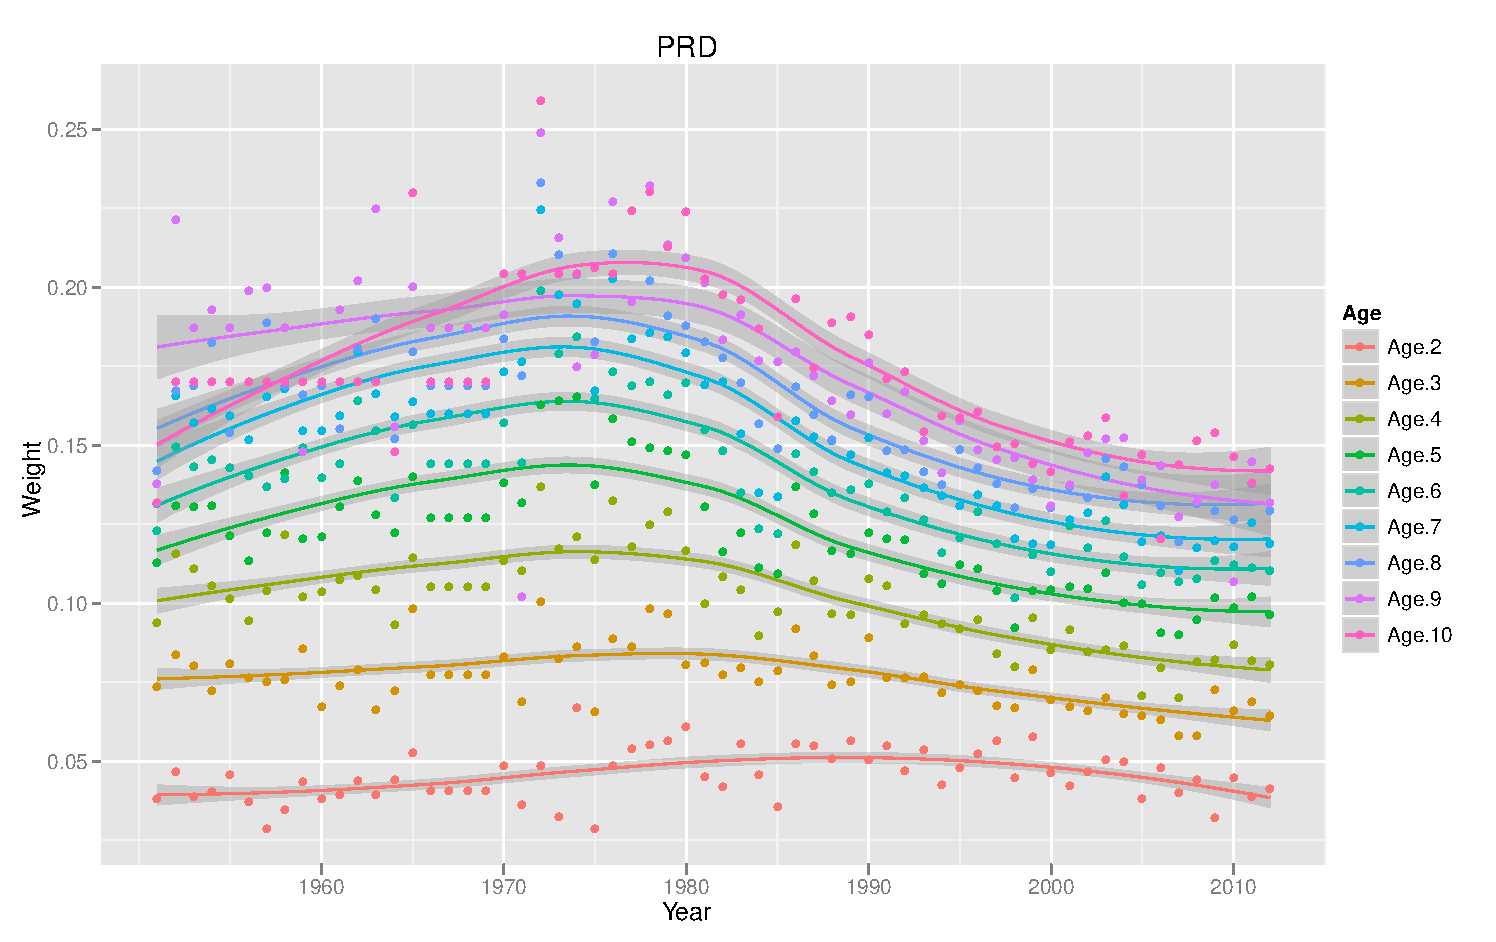
\includegraphics[scale=0.4]
		{../FIGS/iscam_fig_weight-at-age_PRD}
		\caption{Prince Rupert District: empirical weight-at-age (kg).}
	\end{figure}
	}
	%
	\only<3>{
	\begin{figure}[htbp]
		\centering
		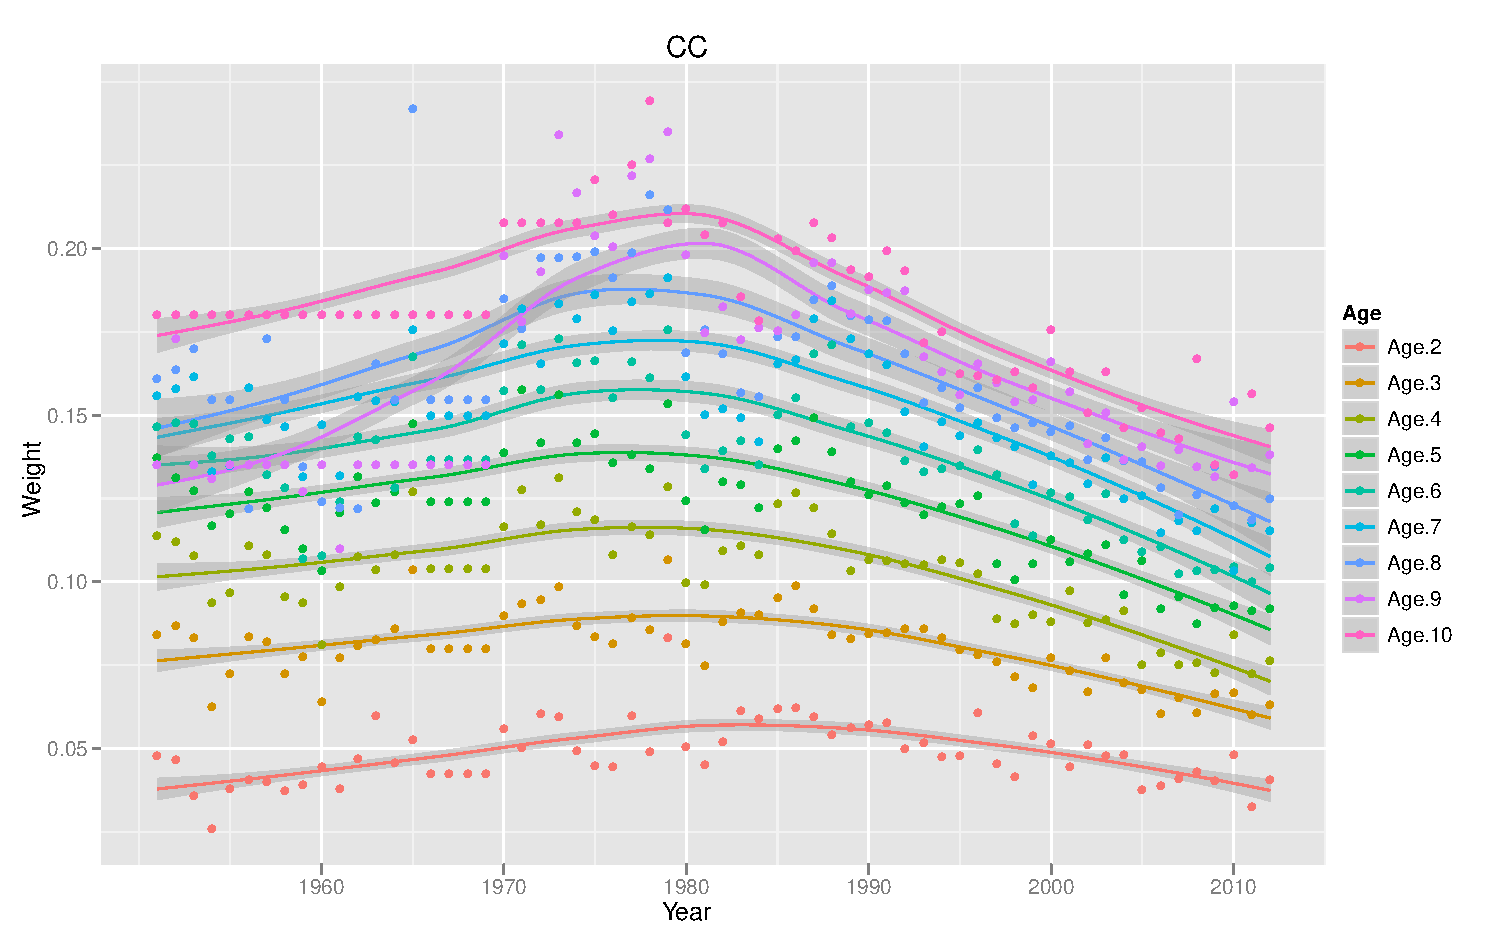
\includegraphics[scale=0.4]
		{../FIGS/iscam_fig_weight-at-age_CC}
		\caption{Central Coast: empirical weight-at-age (kg).}
	\end{figure}
	}
	%
	\only<4>{
	\begin{figure}[htbp]
		\centering
		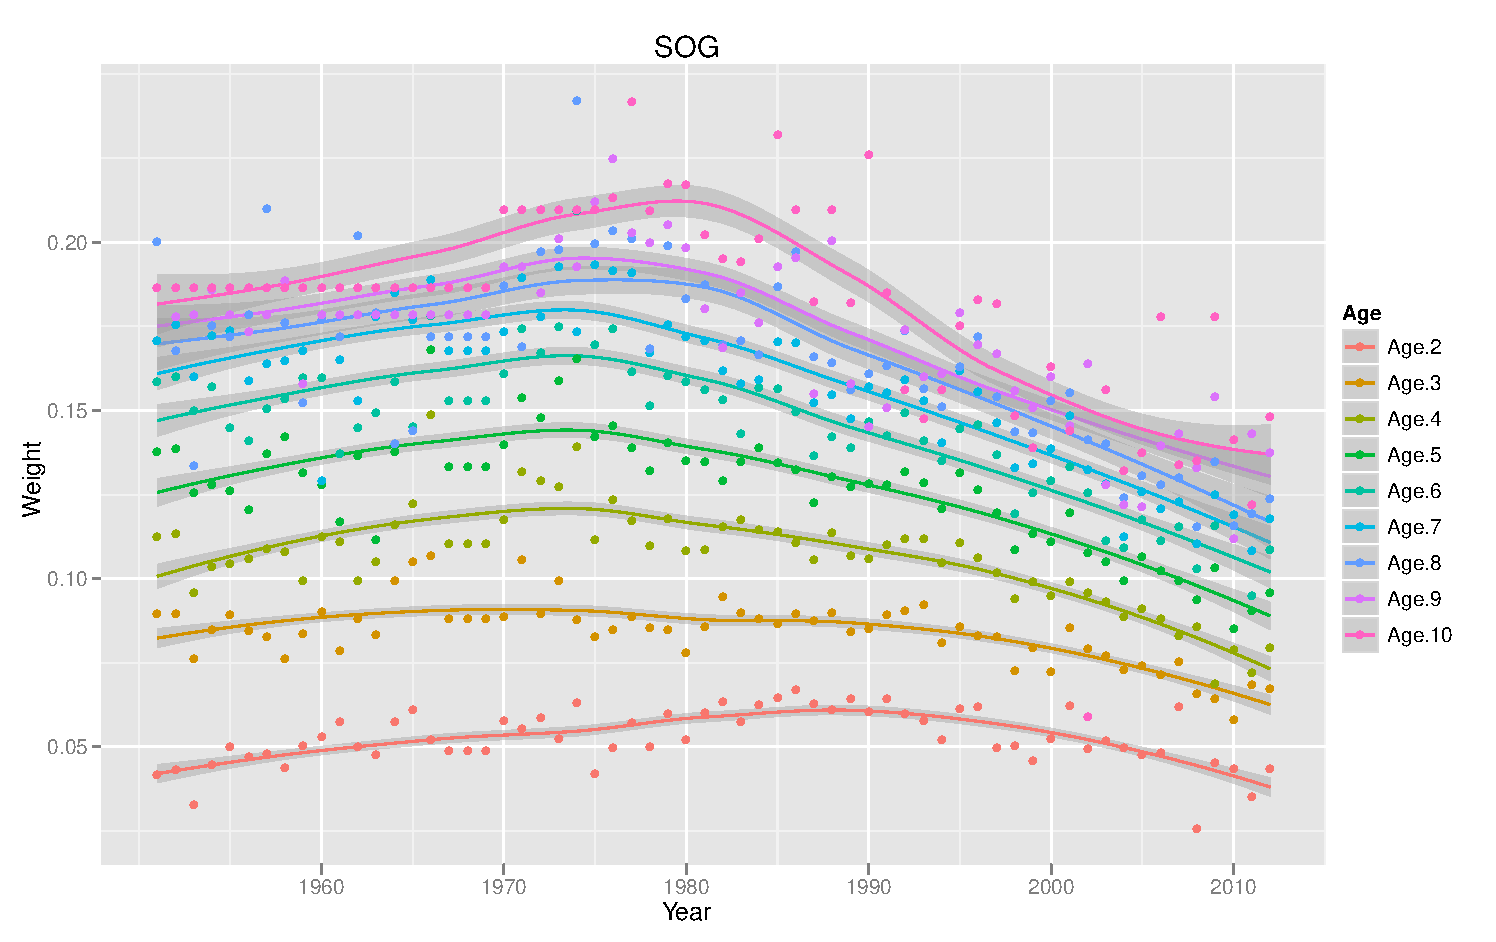
\includegraphics[scale=0.4]
		{../FIGS/iscam_fig_weight-at-age_SOG}
		\caption{Strait of Georgia: empirical weight-at-age (kg).}
	\end{figure}
	}
	%
	\only<5>{
	\begin{figure}[htbp]
		\centering
		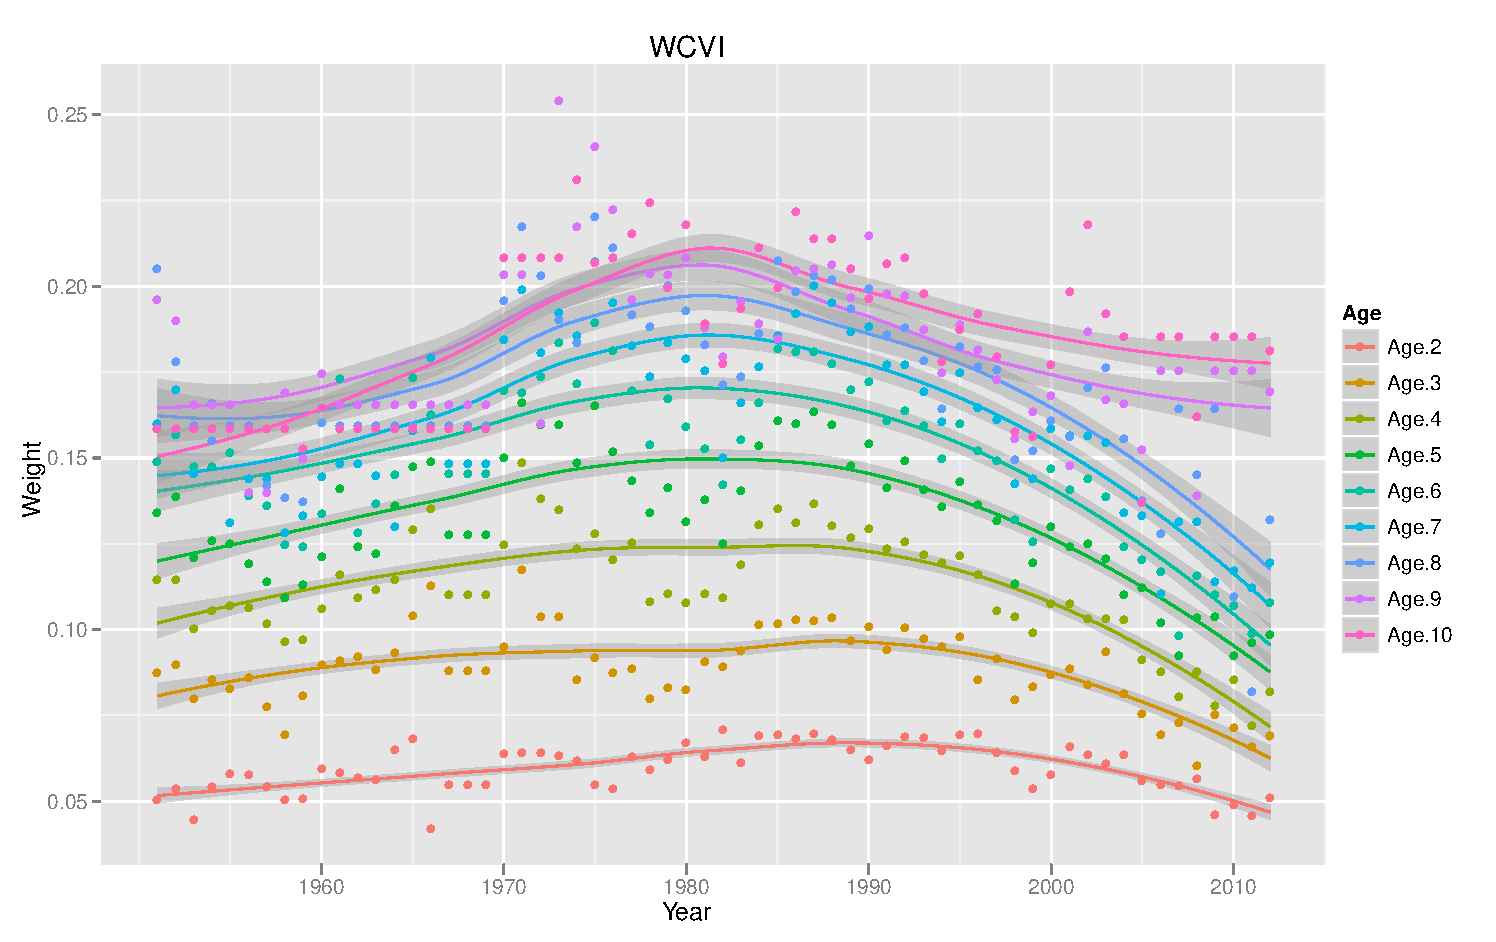
\includegraphics[scale=0.4]
		{../FIGS/iscam_fig_weight-at-age_WCVI}
		\caption{West Coast Vancouver Island: empirical weight-at-age (kg).}
	\end{figure}
	}
	%
\end{frame}
%
% subsection 2011_data (end)

\subsection{Analytical Methods} % (fold)
\label{sub:analytical_methods}
\begin{frame}[t]\frametitle{Analytics \& assumptions}
	\begin{itemize}
		\item<+-> All major and minor areas were assessed using  \iscam.
		\item<+-> Reported catch: CV = 0.005
		\item<+-> Spawn survey: proportional \& 100\% of $Z_t$.
		\item<+-> Dive survey more precise than surface survey.
		\item<+-> Fecundity $\propto$ mature weight-at-age.
		\item<+-> Seine gears: selectivity is asymptotic and time-invariant. 
		\item<+-|alert@+> Gillnet gear: logistic selectivity with weigth-at-age covariates.
		\item<+-|alert@+> $P(\ln(q_1),\ln(q_2)) \sim $ Normal($\mu=-0.569,\sigma=0.274$).
		\item<+-> Homogenous errors in age-composition (multivariate logistic).
		\item<+-> Age-samples $<$0.02 pooled in adjacent cohort.
	\end{itemize}
\end{frame}

\begin{frame}[c]\frametitle{Diagnostics, Forecasts \& Catch Advice}
	\begin{description}
		\item<+->[Diagnostics] Retrospective analysis (sequential removal of the last 10 years of data).
		\item<+->[Forecasts] One-year projection of 3+ biomass with poor, average, good age-3 recruitment.
		\item<+->[Catch advice] Based on HCR with 20\% harvest rate if above cutoff.
	\end{description}
\end{frame}
% subsection analytical_methods (end)

\subsection{Maximum Likelihood Estimates} % (fold)
\label{sub:maximum_likelihood_estimates}
%
\begin{frame}[t]\frametitle{MLE: Spawn survey}
	\only<1>{
	\begin{figure}[htbp]
		\centering
		\vspace{-1cm}
		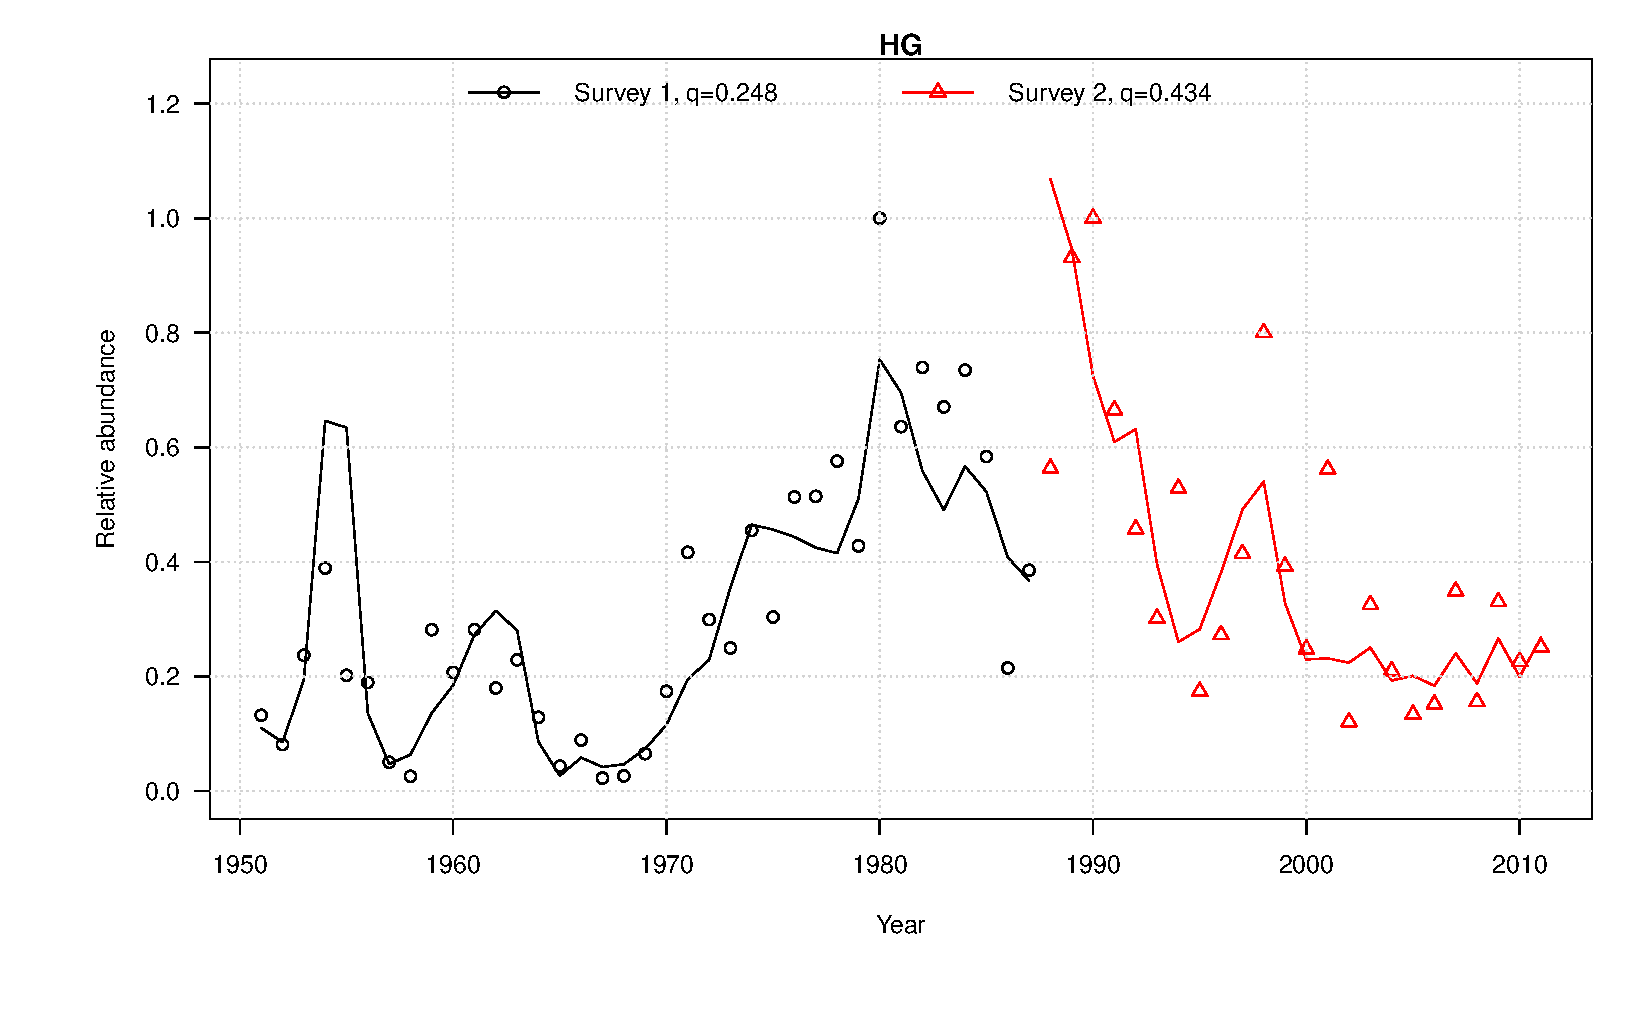
\includegraphics[scale=0.4]
	{../FIGS/qPriorFigs/iscam_fig_survey_fit_HG}
		\vspace{-1cm}
		\caption{Haida Gwaii}
	\end{figure}
	}
	%
	\only<2>{
	\begin{figure}[htbp]
		\centering
		\vspace{-1cm}
		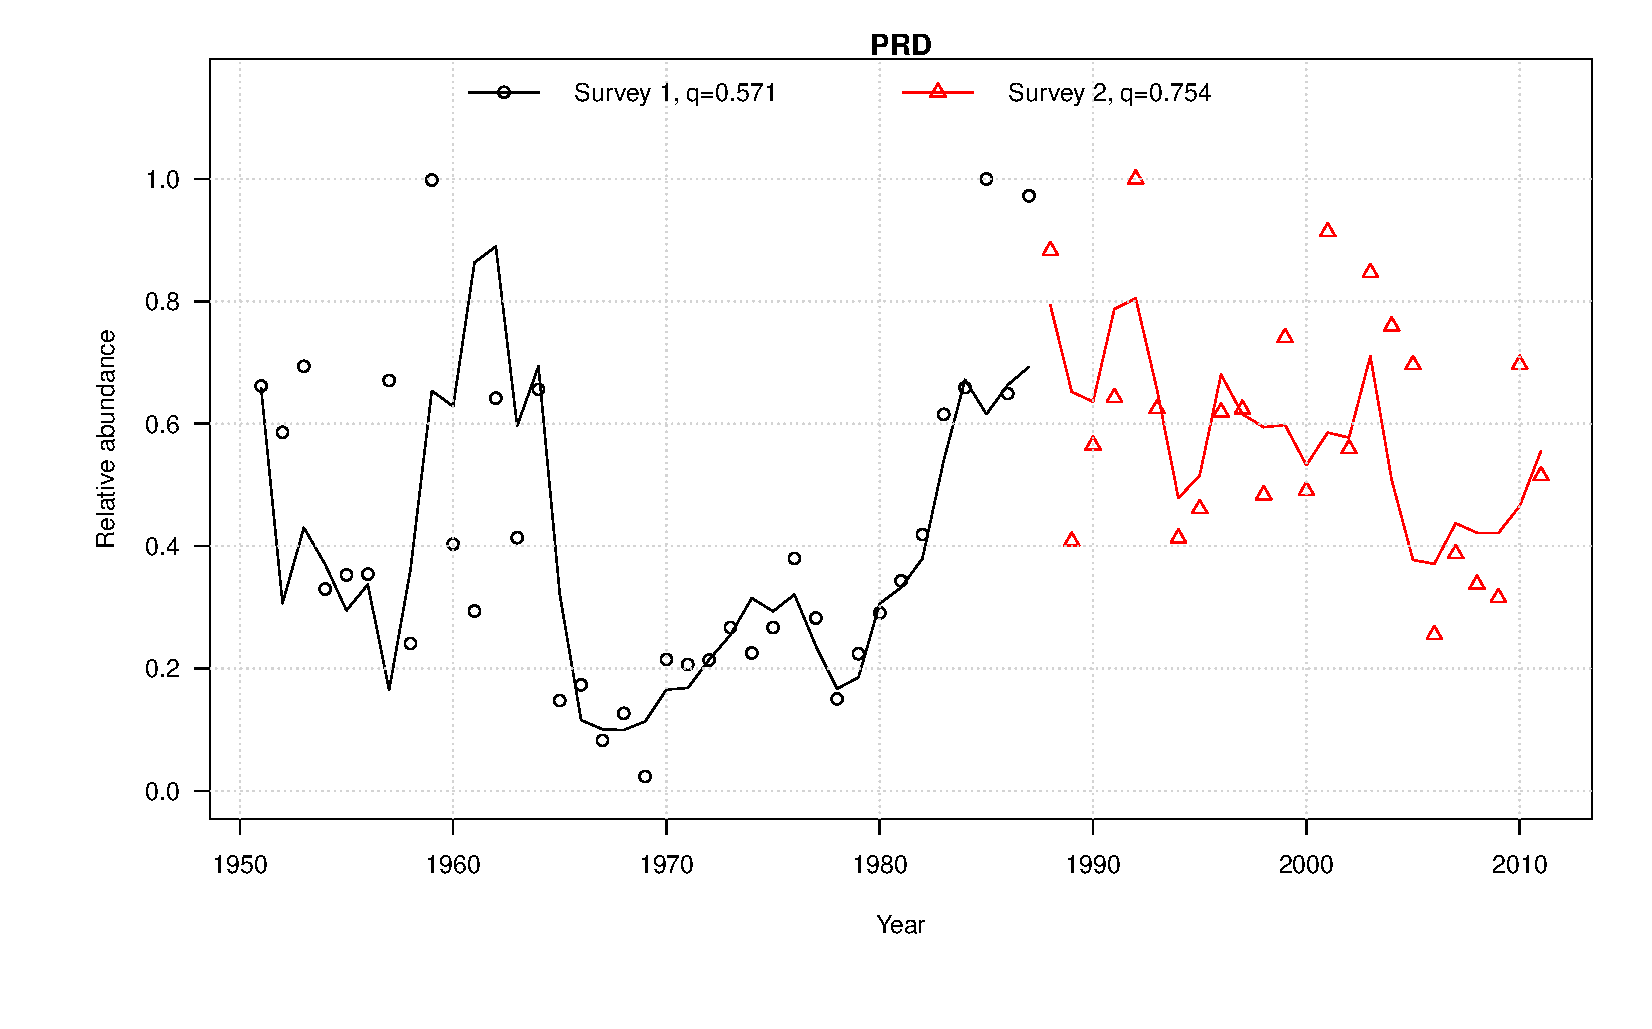
\includegraphics[scale=0.4]
	{../FIGS/qPriorFigs/iscam_fig_survey_fit_PRD}
		\vspace{-1cm}
		\caption{Prince Rupert District}
	\end{figure}
	}
	%
	\only<3>{
	\begin{figure}[htbp]
		\centering
		\vspace{-1cm}
		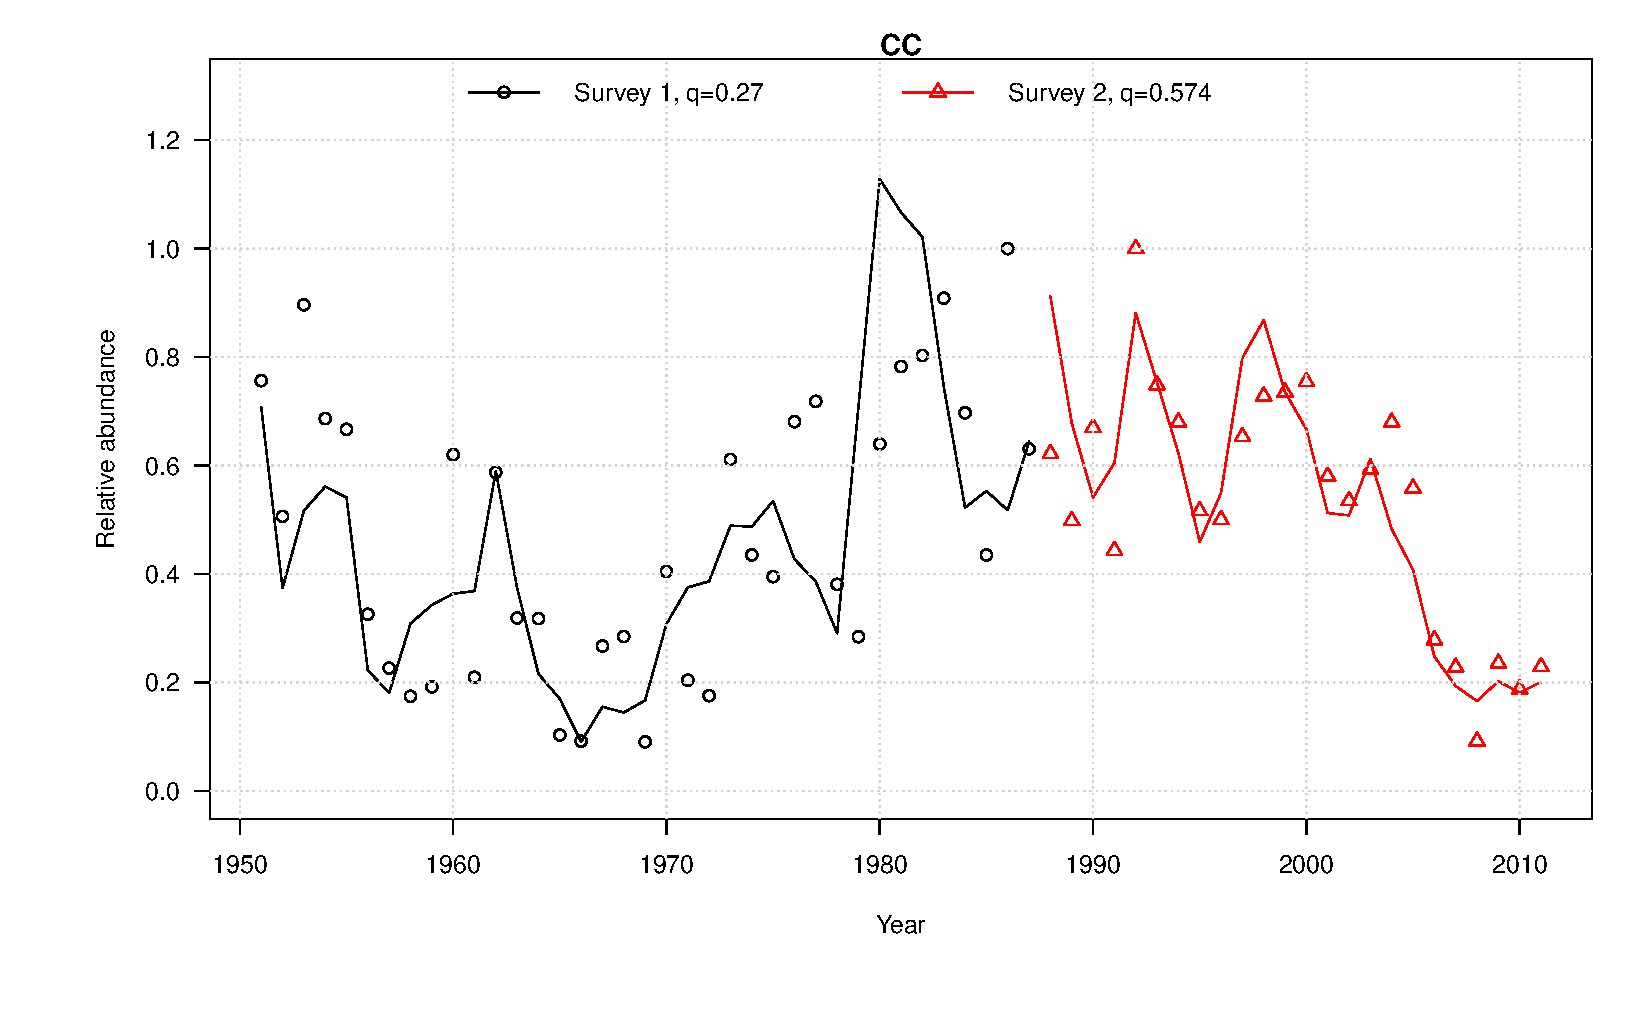
\includegraphics[scale=0.4]
	{../FIGS/qPriorFigs/iscam_fig_survey_fit_CC}
		\vspace{-1cm}
		\caption{Central Coast}
	\end{figure}
	}
	%
	\only<4>{
	\begin{figure}[htbp]
		\centering
		\vspace{-1cm}
		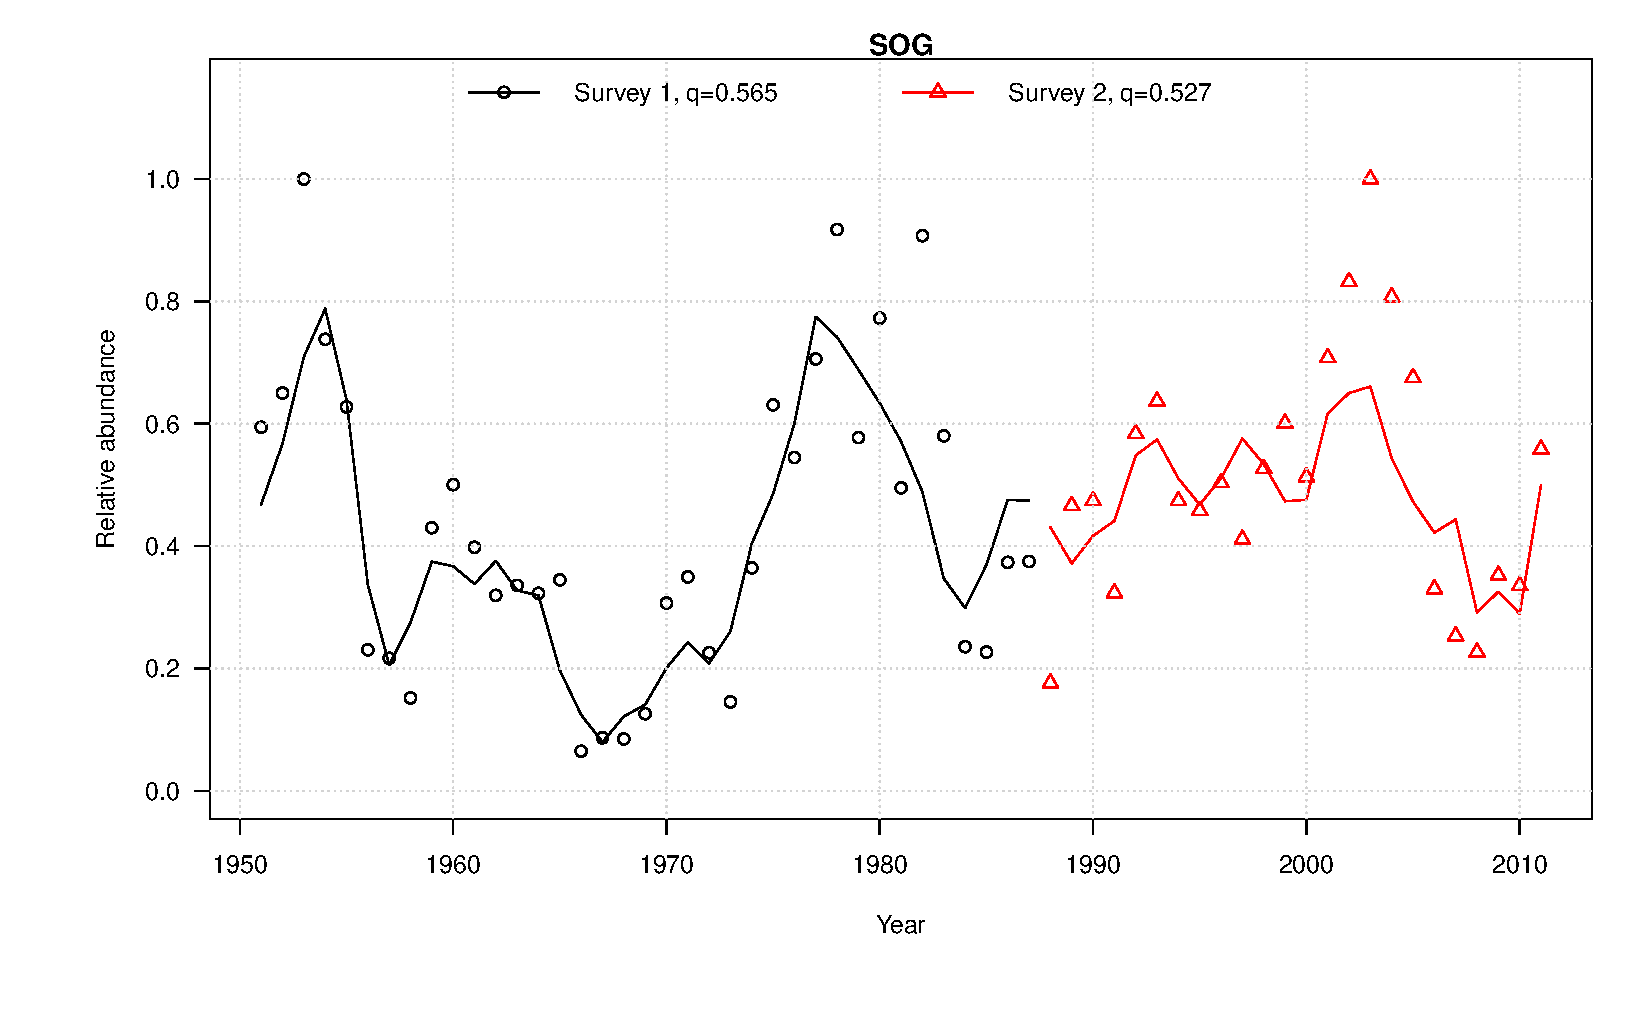
\includegraphics[scale=0.4]
	{../FIGS/qPriorFigs/iscam_fig_survey_fit_SOG}
		\vspace{-1cm}
		\caption{Strait of Georgia}
	\end{figure}
	}
	%
	\only<5>{
	\begin{figure}[htbp]
		\centering
		\vspace{-1cm}
		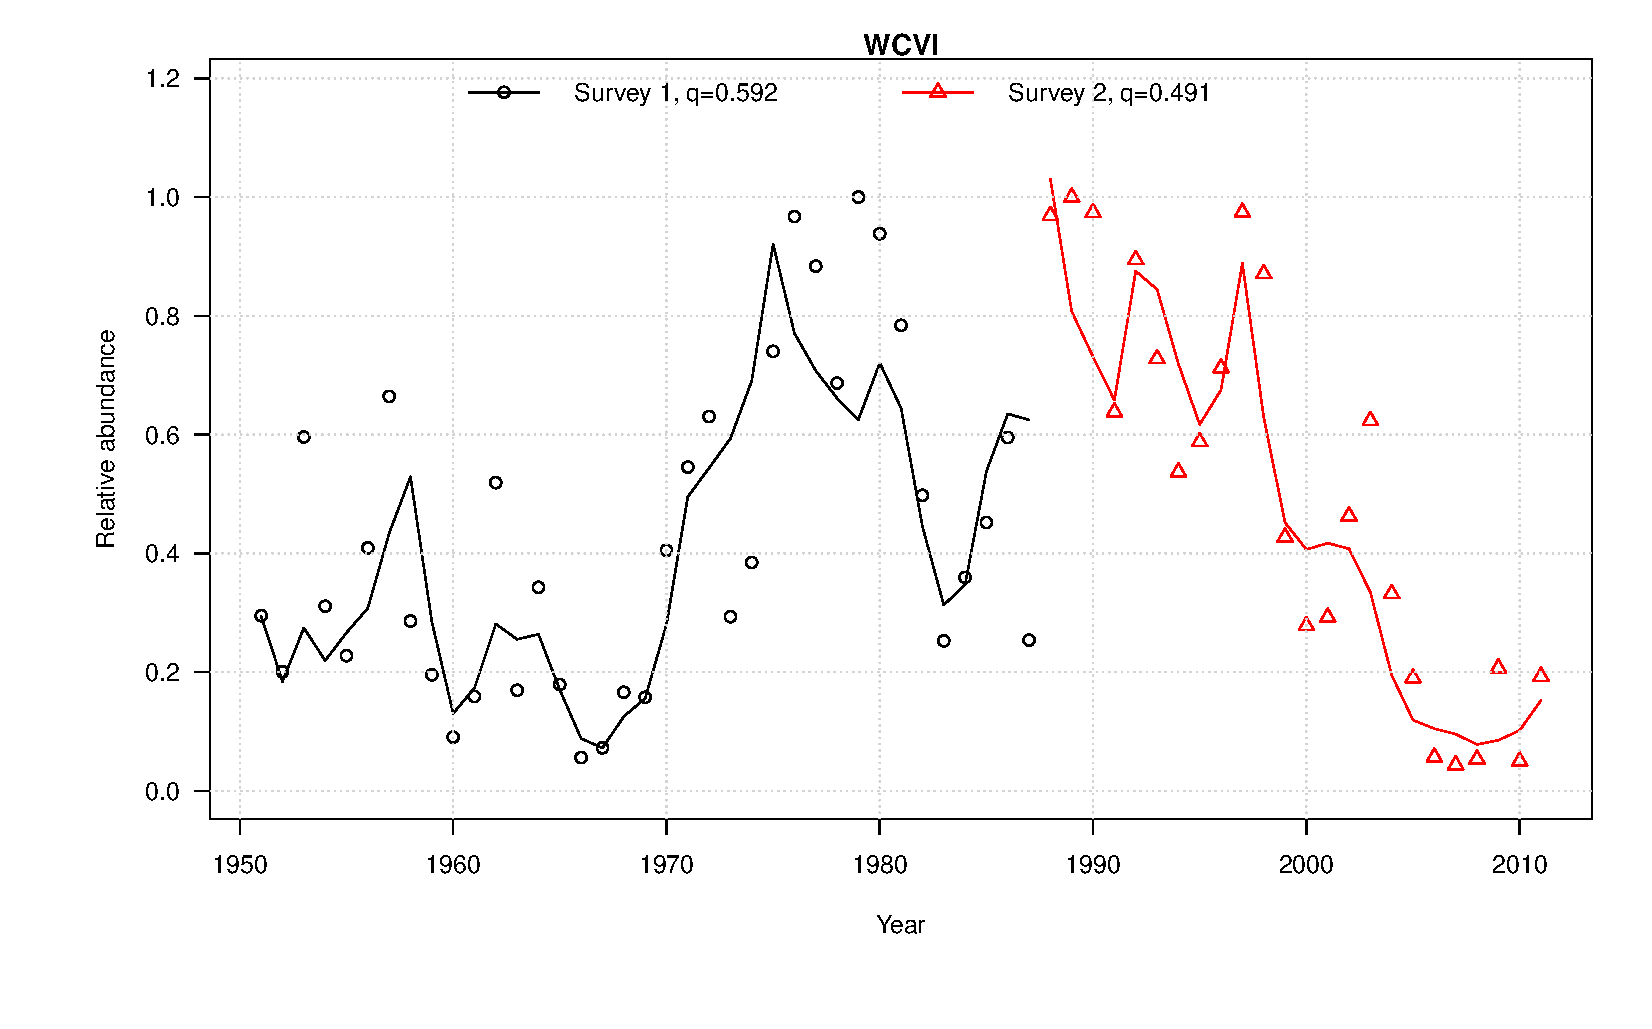
\includegraphics[scale=0.4]
	{../FIGS/qPriorFigs/iscam_fig_survey_fit_WCVI}
		\vspace{-1cm}
		\caption{West Coast Vancouver Island}
	\end{figure}
	}
	%
\end{frame}
%
\begin{frame}[t]\frametitle{MLE: Residuals in age composition data}
	\only<1>{
	\begin{figure}[htbp]
		\centering
		\vspace{-.75cm}
		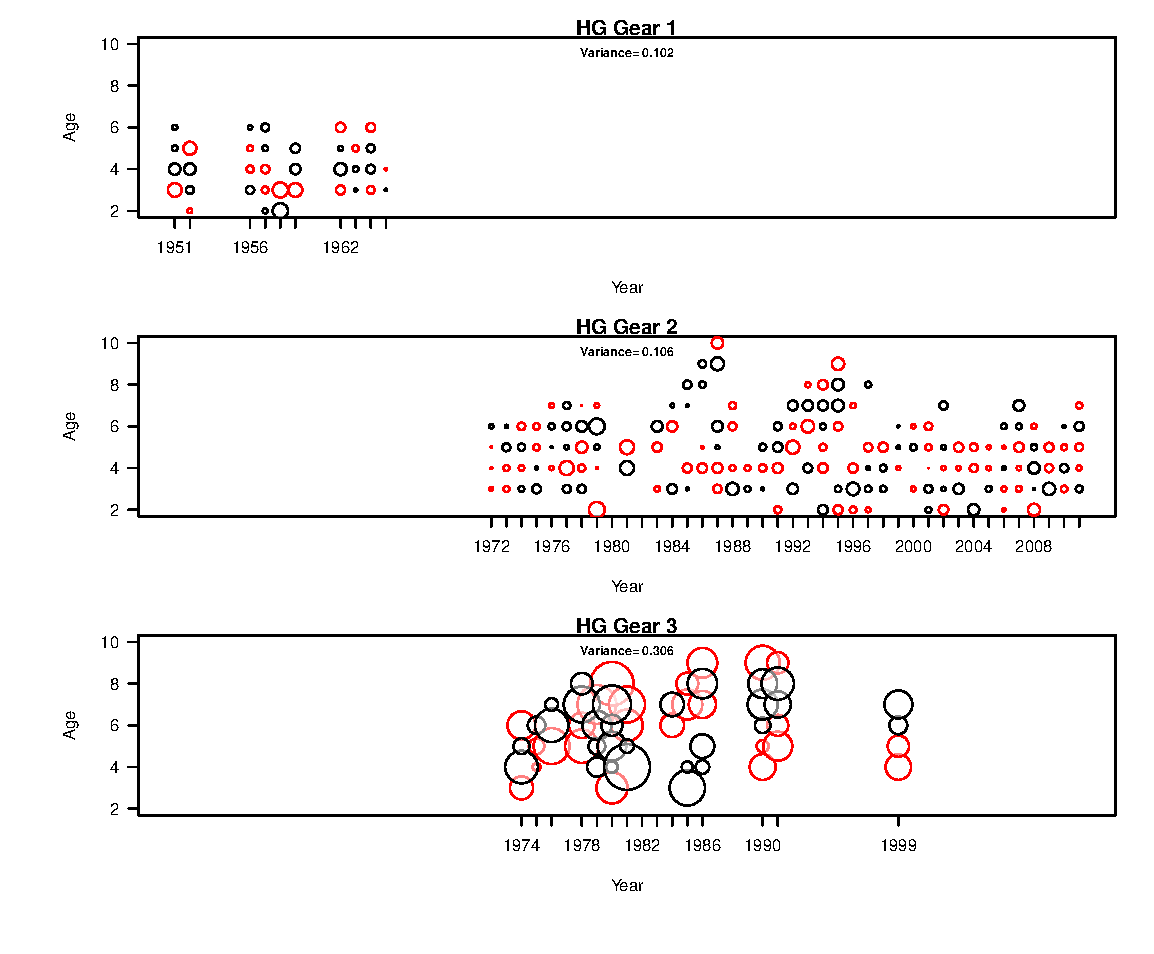
\includegraphics[scale=0.5]
	{../FIGS/qPriorFigs/iscam_fig_agecompsresid_HG}
		\vspace{-1cm}
		\caption{Haida Gwaii}
	\end{figure}
	}
	%
	\only<2>{
	\begin{figure}[htbp]
		\centering
		\vspace{-.75cm}
		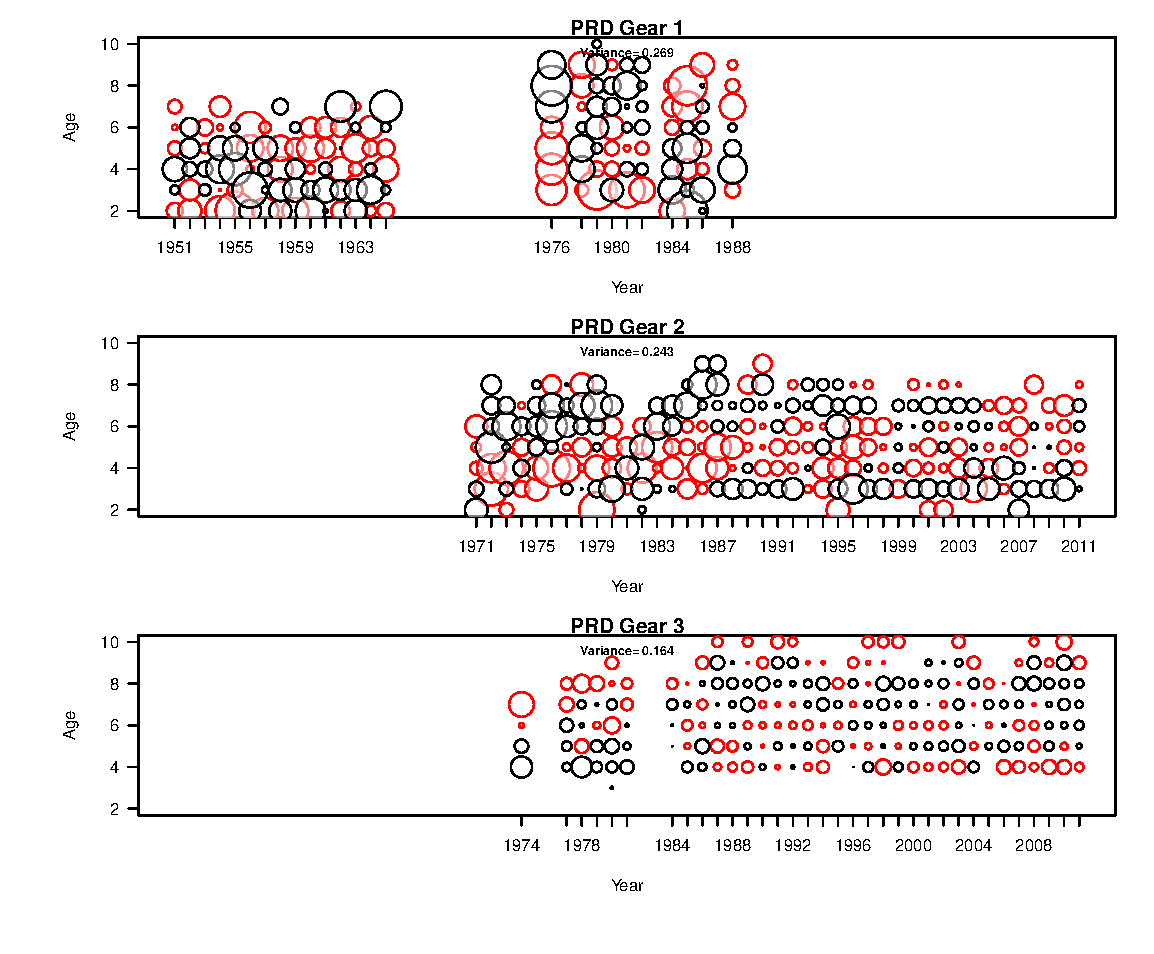
\includegraphics[scale=0.5]
	{../FIGS/qPriorFigs/iscam_fig_agecompsresid_PRD}
		\vspace{-1cm}
		\caption{Prince Rupert District}
	\end{figure}
	}
	%
	\only<3>{
	\begin{figure}[htbp]
		\centering
		\vspace{-.75cm}
		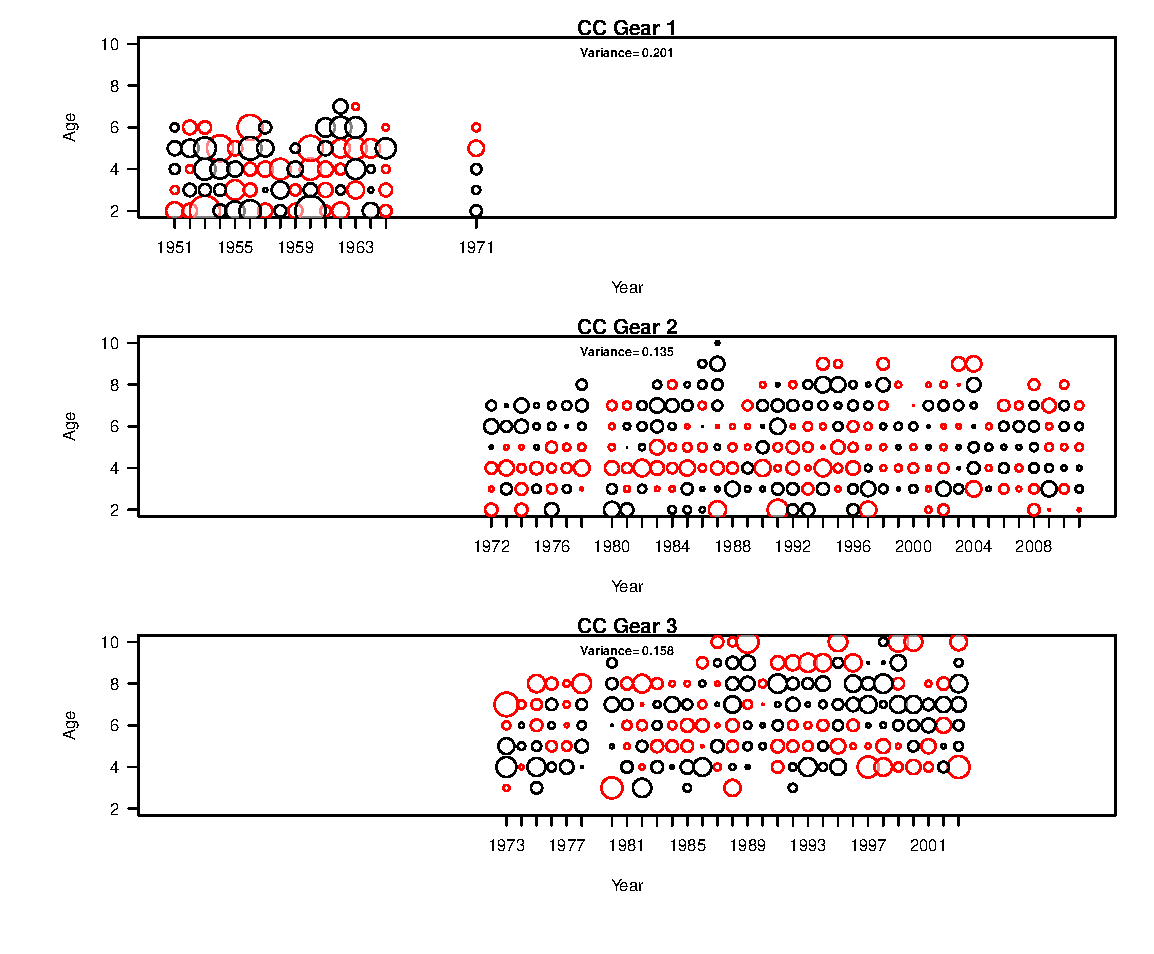
\includegraphics[scale=0.5]
	{../FIGS/qPriorFigs/iscam_fig_agecompsresid_CC}
		\vspace{-1cm}
		\caption{Central Coast}
	\end{figure}
	}
	%
	\only<4>{
	\begin{figure}[htbp]
		\centering
		\vspace{-.75cm}
		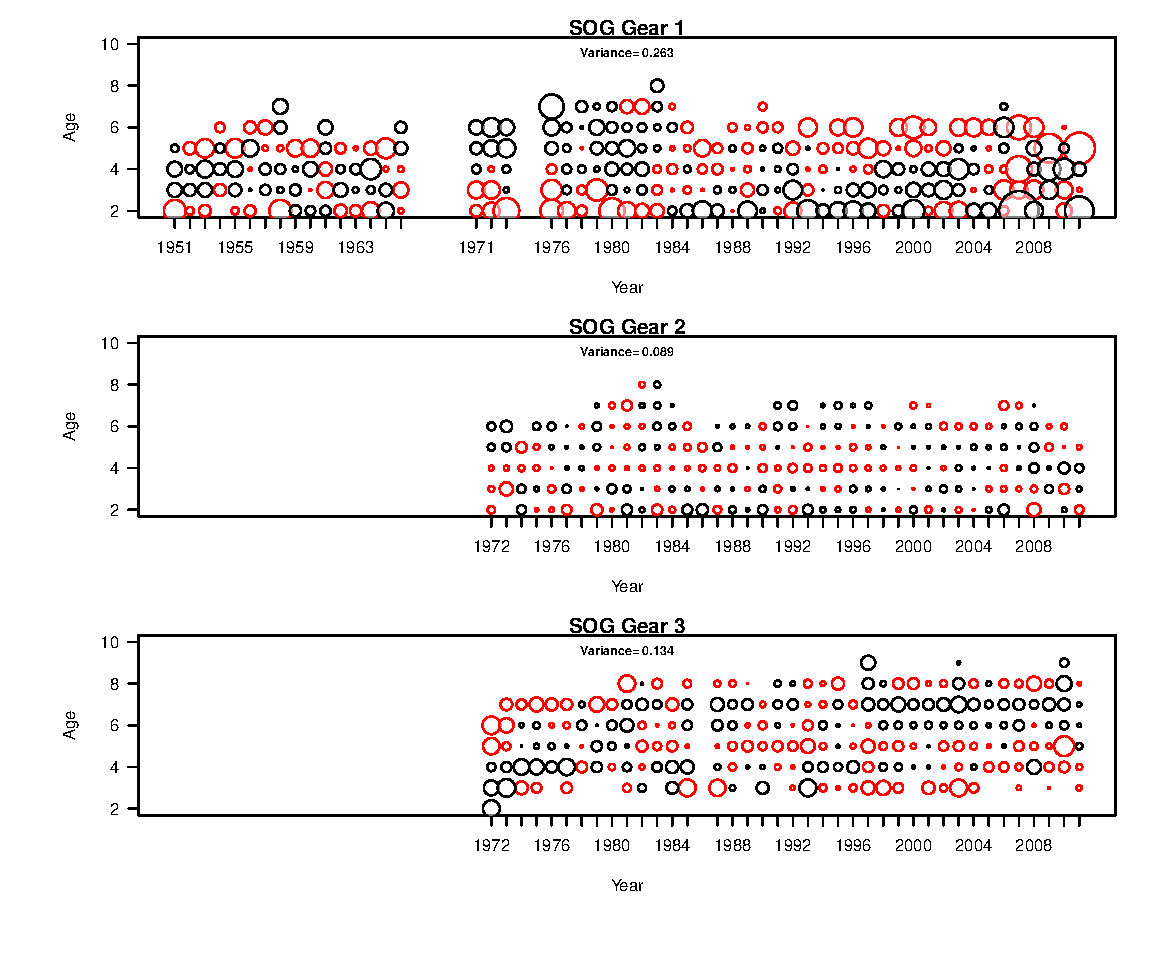
\includegraphics[scale=0.5]
	{../FIGS/qPriorFigs/iscam_fig_agecompsresid_SOG}
		\vspace{-1cm}
		\caption{Strait of Georgia}
	\end{figure}
	}
	%
	\only<5>{
	\begin{figure}[htbp]
		\centering
		\vspace{-.75cm}
		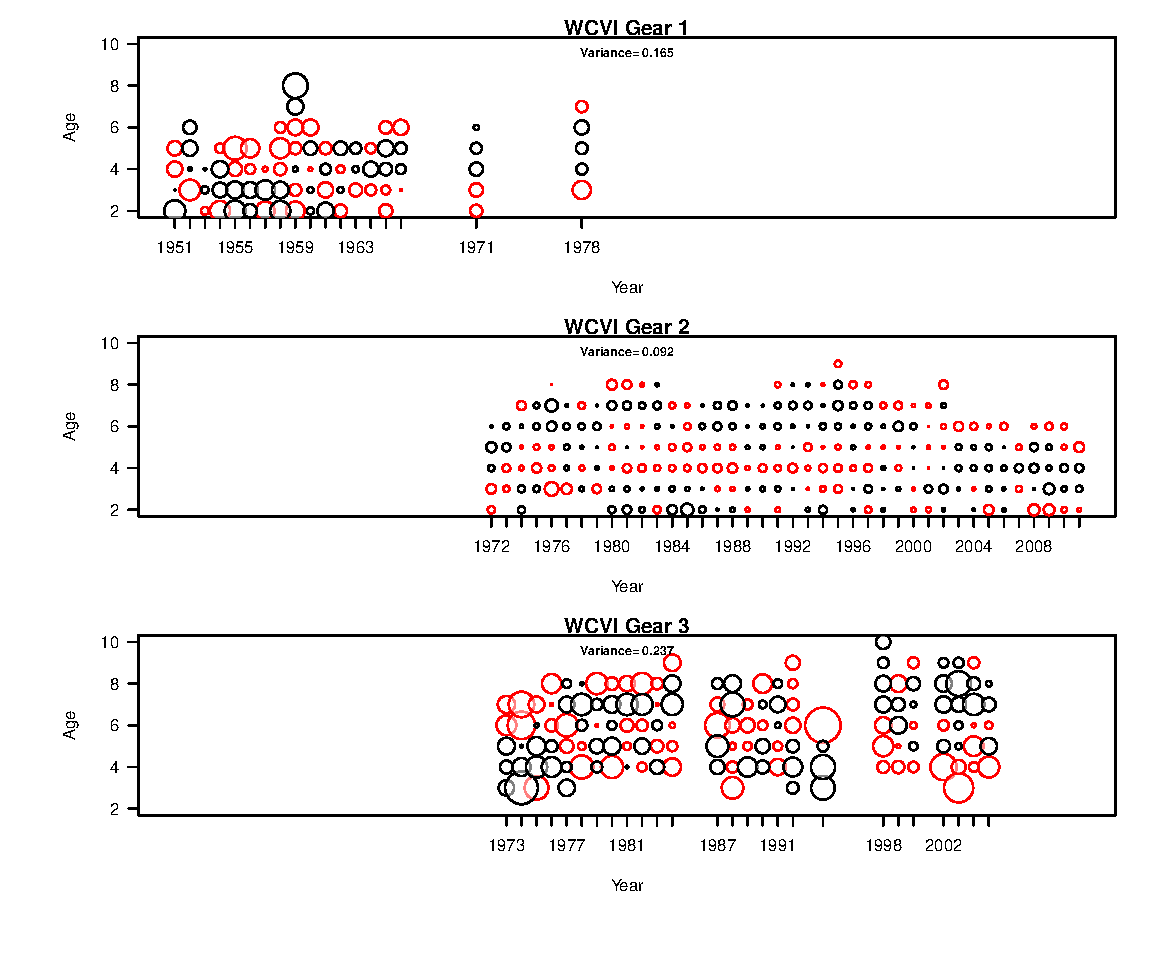
\includegraphics[scale=0.5]
	{../FIGS/qPriorFigs/iscam_fig_agecompsresid_WCVI}
		\vspace{-1cm}
		\caption{West Coast Vancouver Island}
	\end{figure}
	}
	%
\end{frame}
%
\begin{frame}[t]\frametitle{MLE: Mortality}
	\only<1>{
	\begin{figure}[htbp]
		\centering
		\vspace{-1cm}
		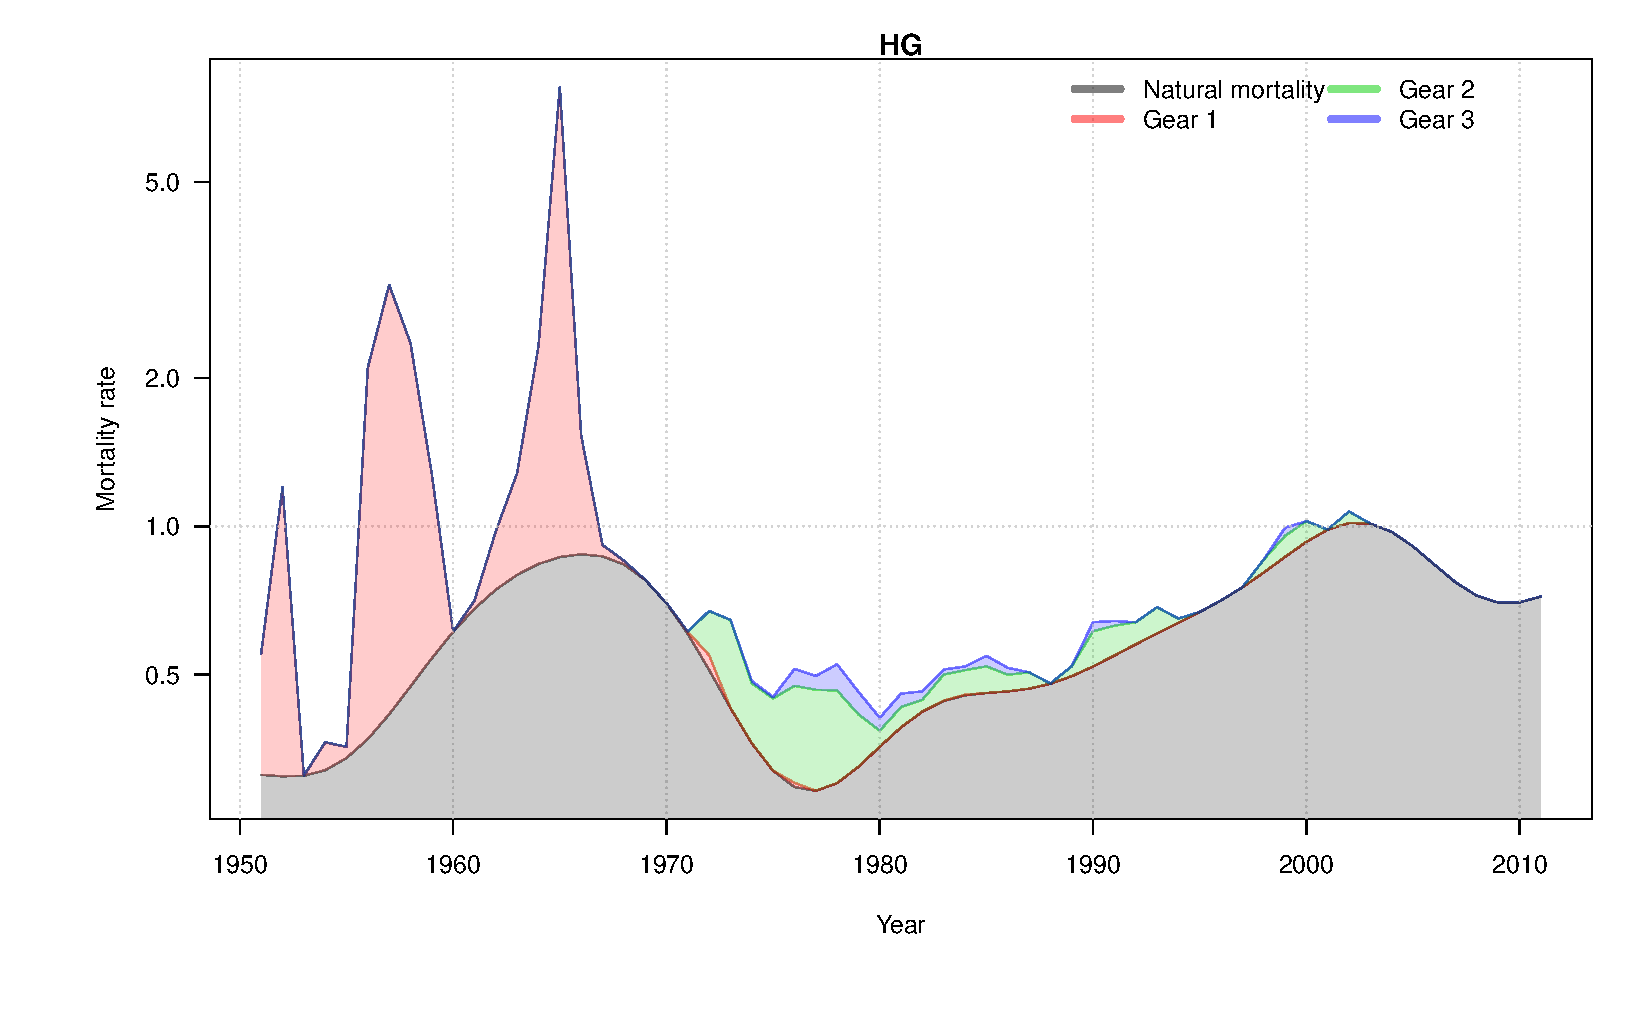
\includegraphics[scale=0.4]
	{../FIGS/qPriorFigs/iscam_fig_mortality_HG}
		\vspace{-1cm}
		\caption{Haida Gwaii}
	\end{figure}
	}
	%
	\only<2>{
	\begin{figure}[htbp]
		\centering
		\vspace{-1cm}
		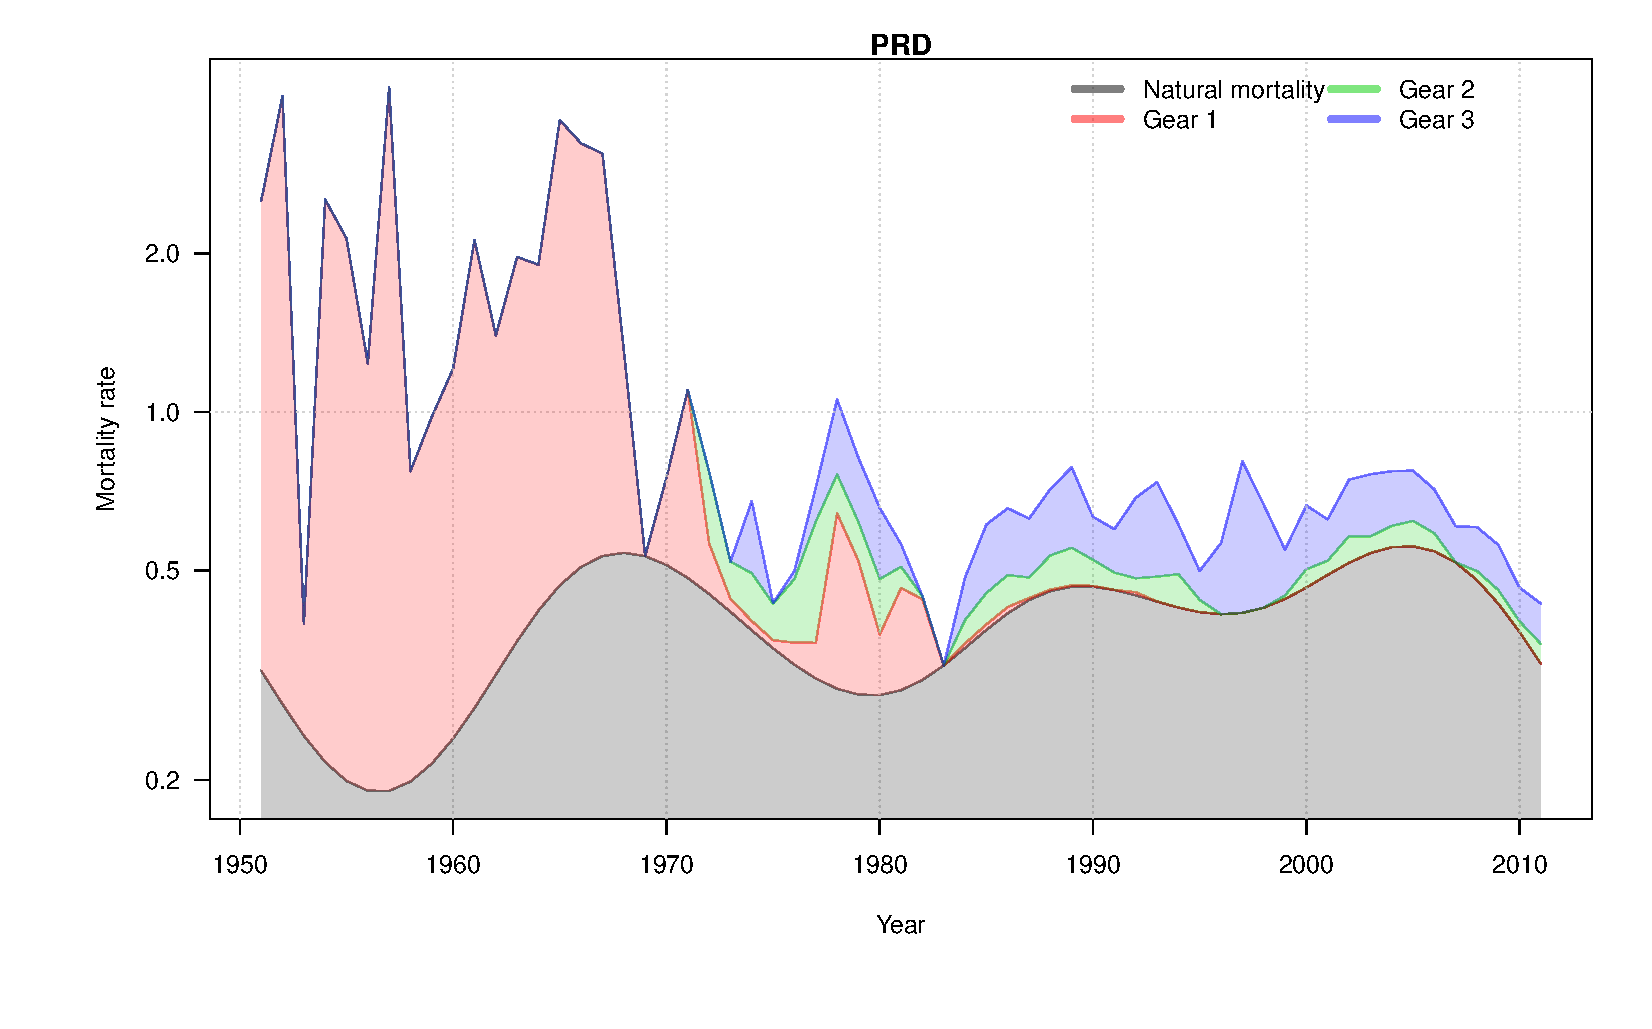
\includegraphics[scale=0.4]
	{../FIGS/qPriorFigs/iscam_fig_mortality_PRD}
		\vspace{-1cm}
		\caption{Prince Rupert District}
	\end{figure}
	}
	%
	\only<3>{
	\begin{figure}[htbp]
		\centering
		\vspace{-1cm}
		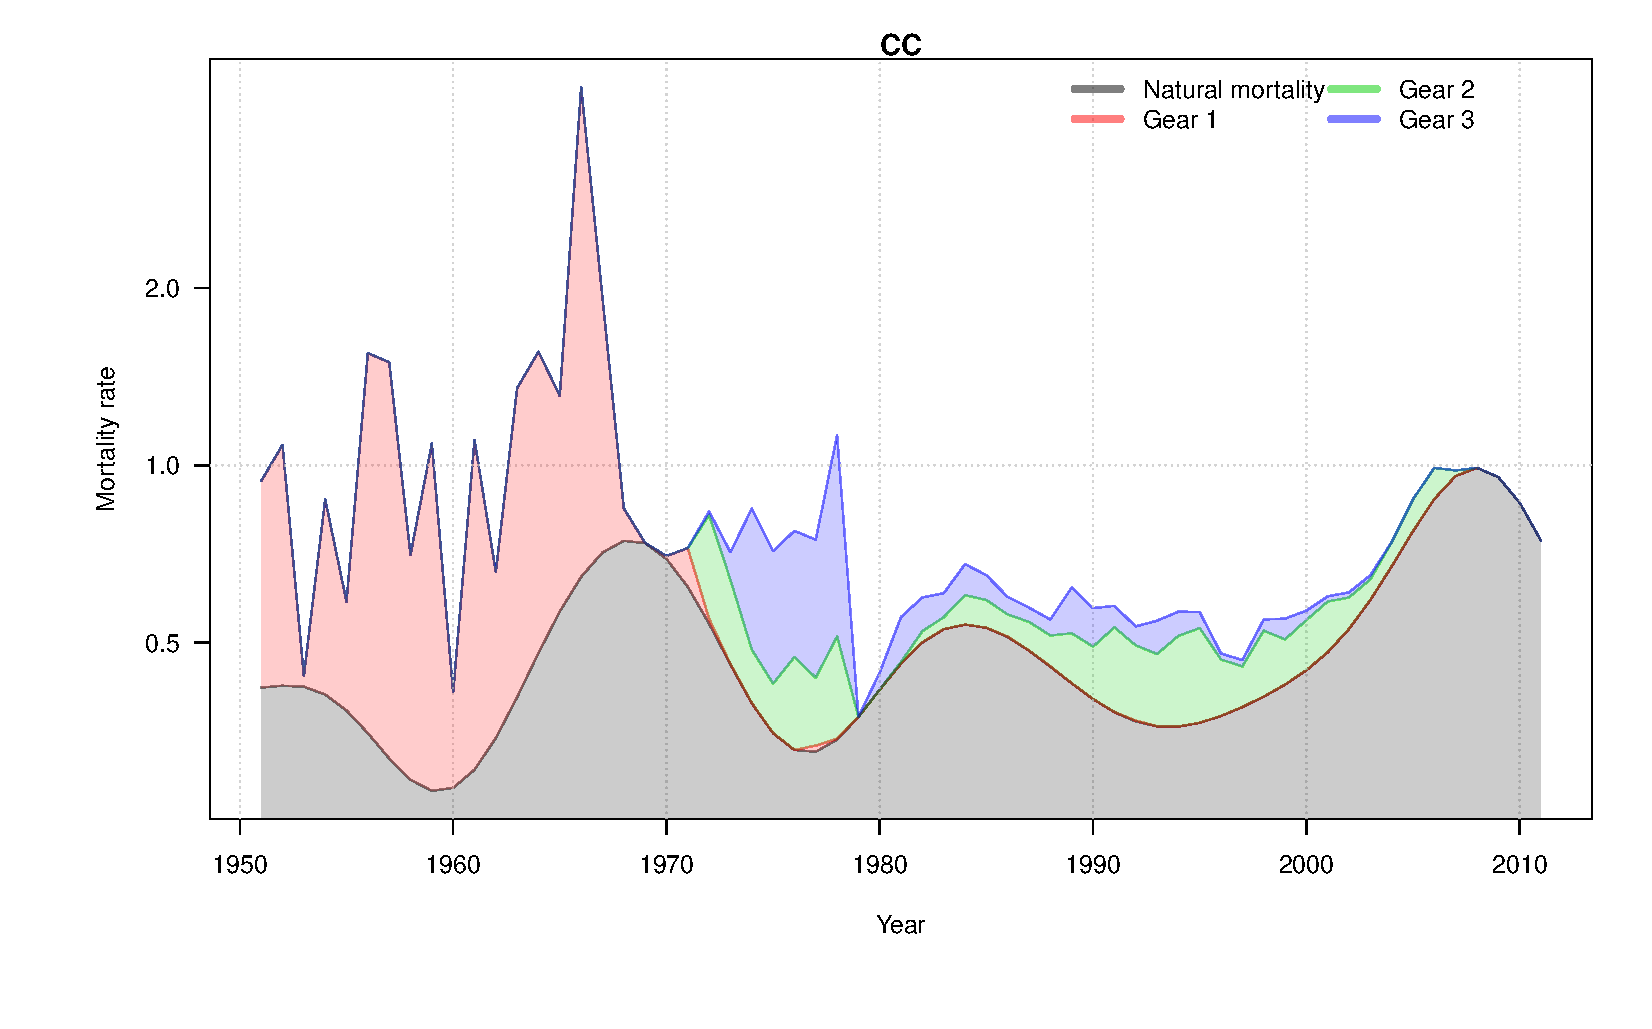
\includegraphics[scale=0.4]
	{../FIGS/qPriorFigs/iscam_fig_mortality_CC}
		\vspace{-1cm}
		\caption{Central Coast}
	\end{figure}
	}
	%
	\only<4>{
	\begin{figure}[htbp]
		\centering
		\vspace{-1cm}
		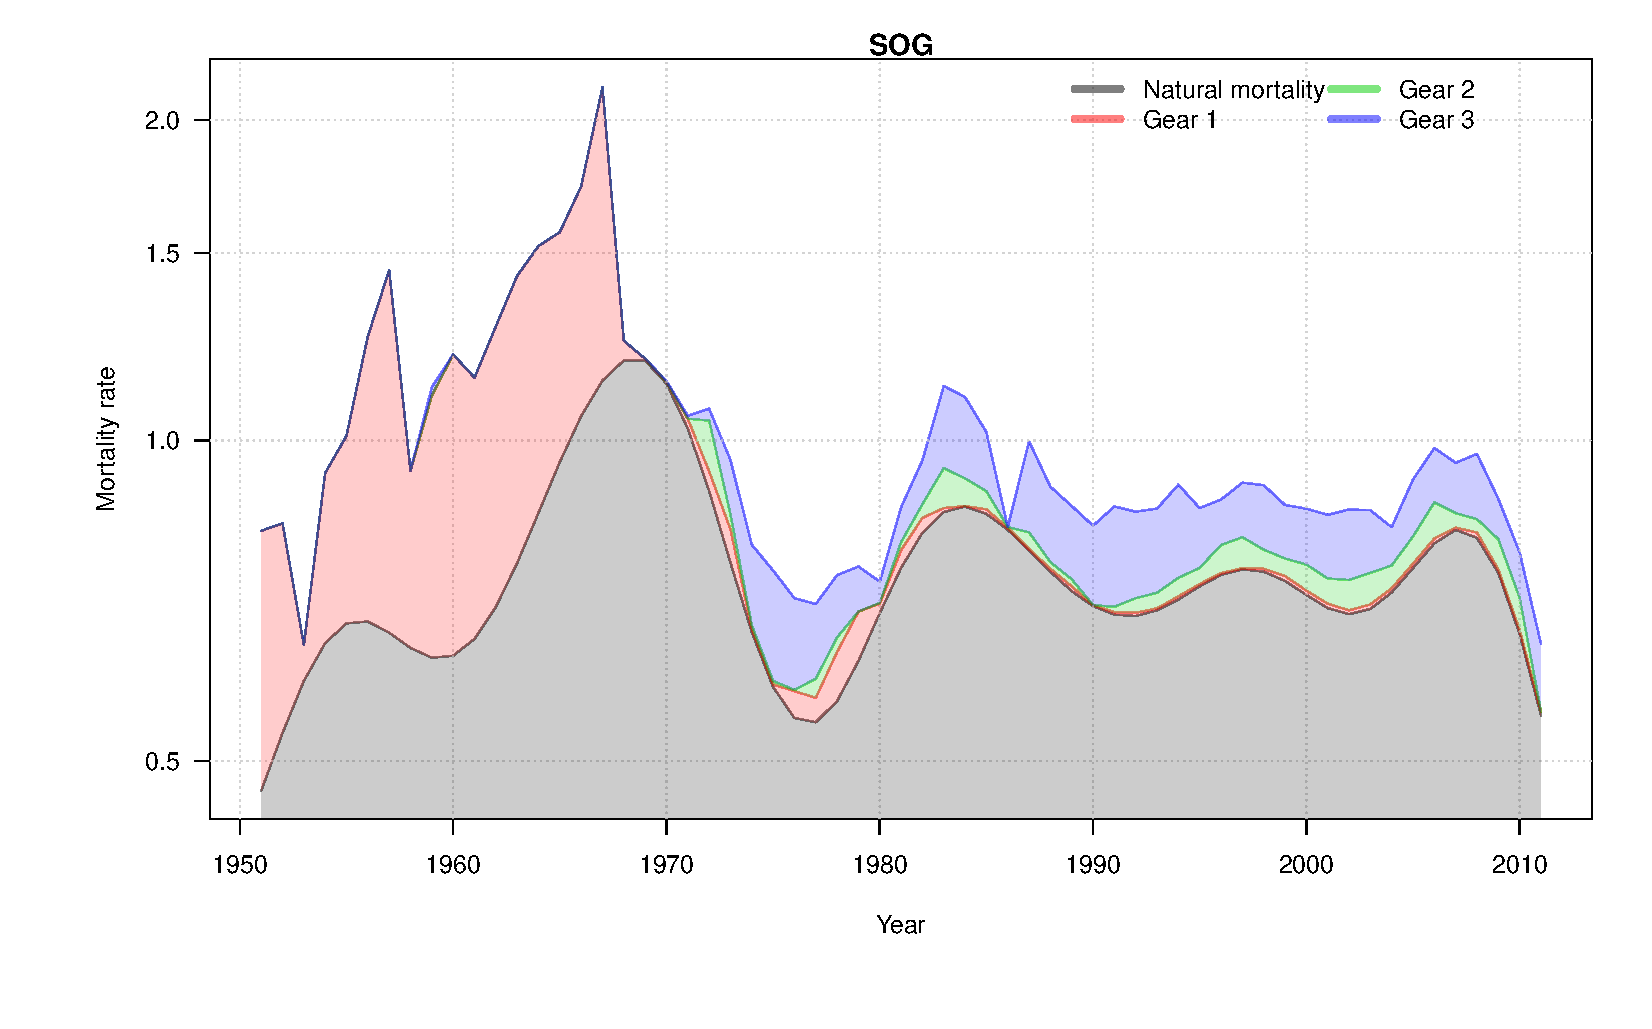
\includegraphics[scale=0.4]
	{../FIGS/qPriorFigs/iscam_fig_mortality_SOG}
		\vspace{-1cm}
		\caption{Strait of Georgia}
	\end{figure}
	}
	%
	\only<5>{
	\begin{figure}[htbp]
		\centering
		\vspace{-1cm}
		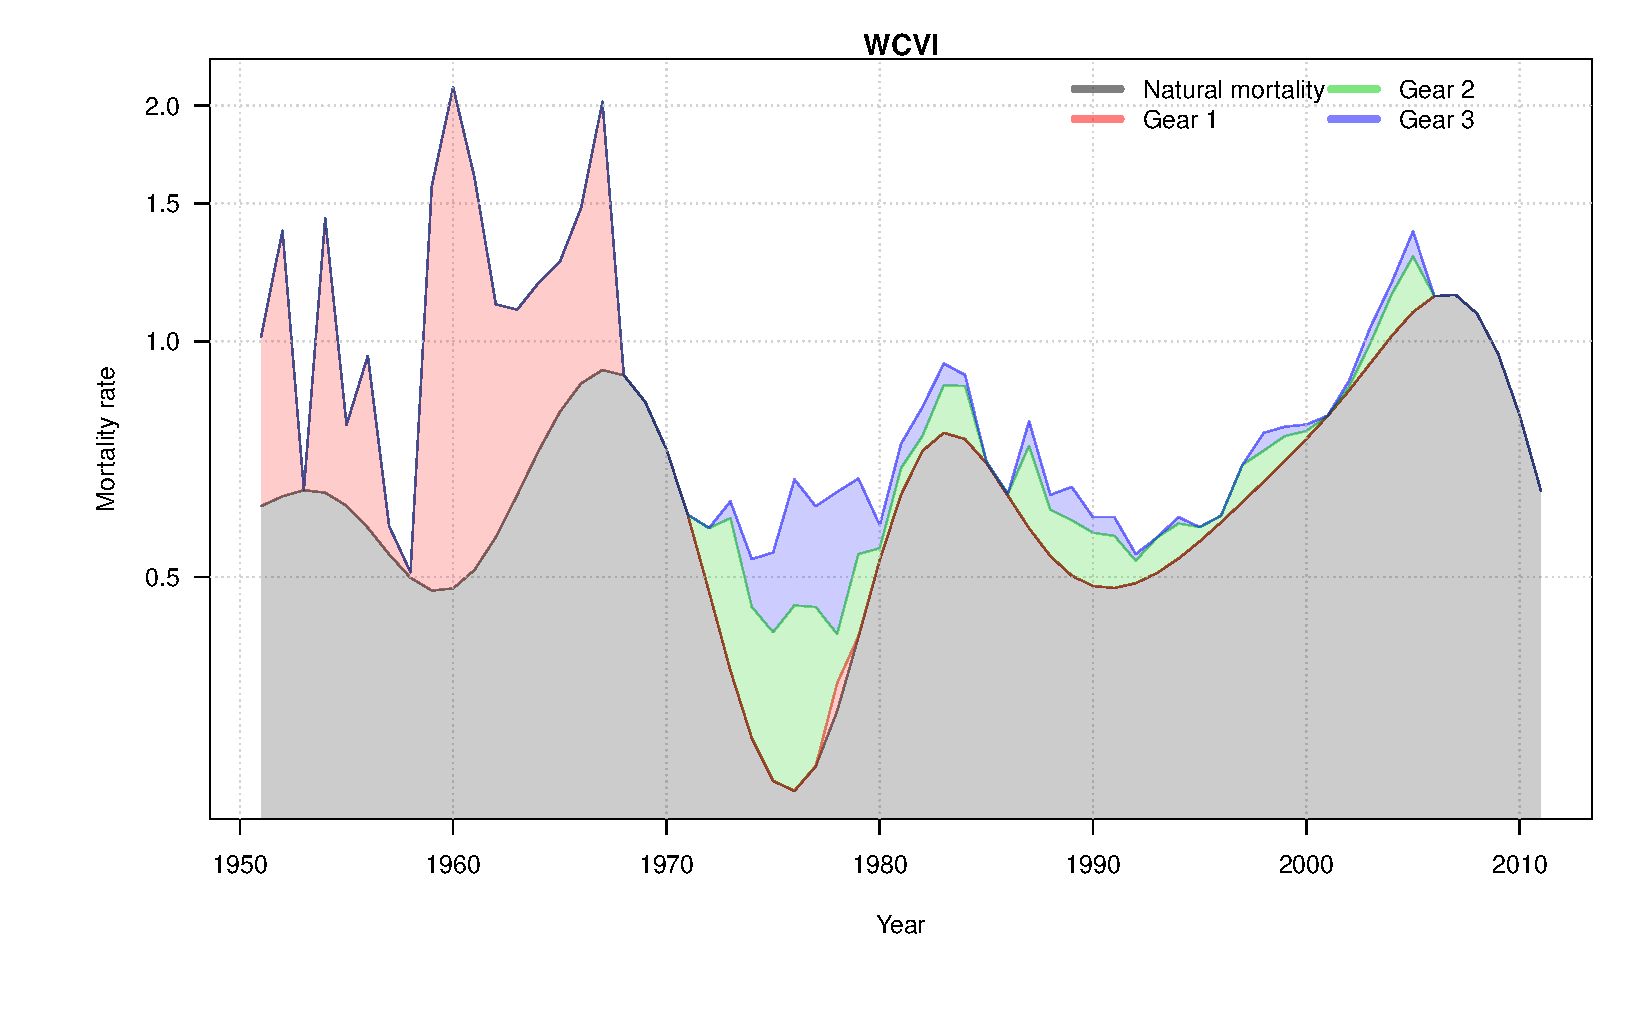
\includegraphics[scale=0.4]
	{../FIGS/qPriorFigs/iscam_fig_mortality_WCVI}
		\vspace{-1cm}
		\caption{West Coast Vancouver Island}
	\end{figure}
	}
	%
\end{frame}
%
\begin{frame}[t]\frametitle{Age-2 recruits}
	\begin{figure}[htbp]
		\centering
		\vspace{-1cm}	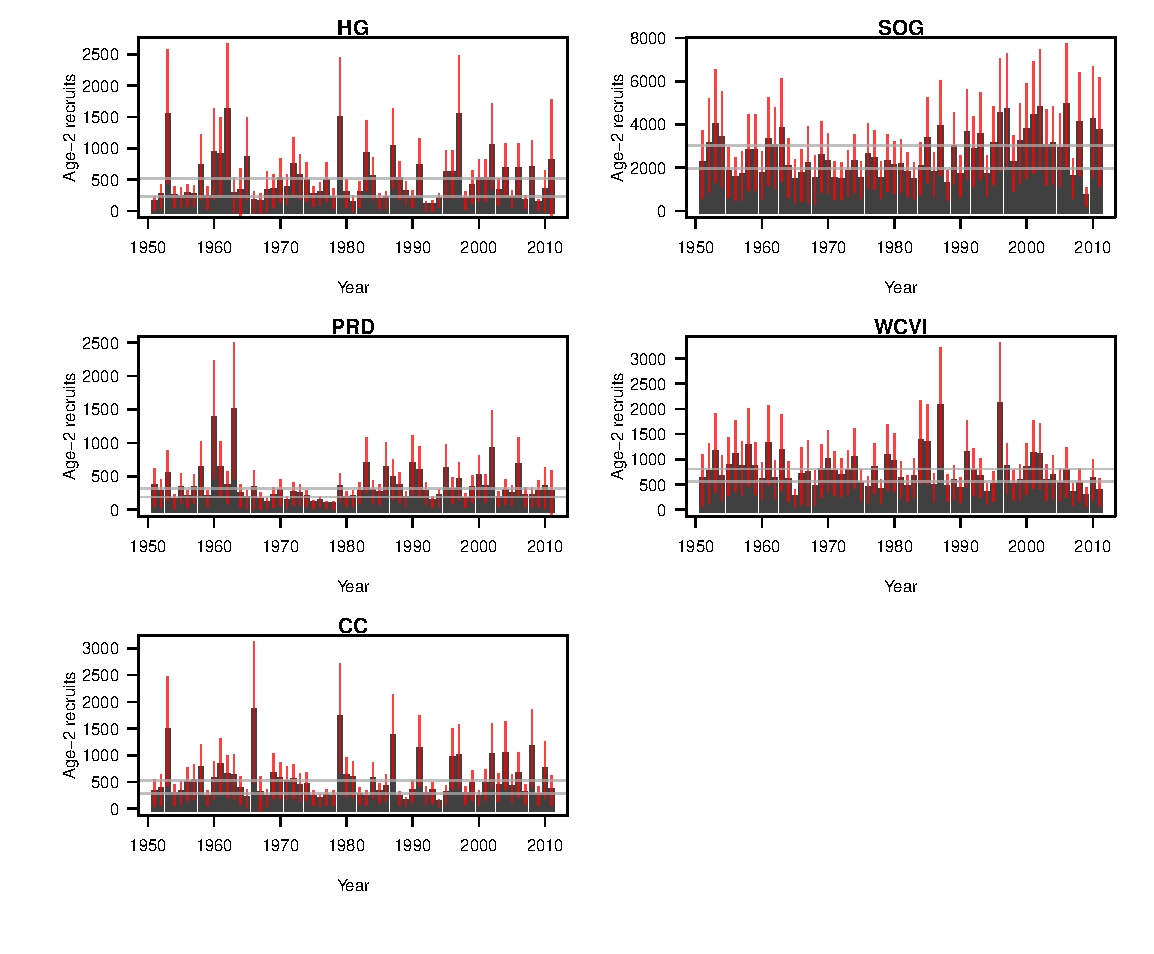
\includegraphics[scale=0.5]{../FIGS/qPriorFigs/iscam_fig_recruitment}
		\vspace{-1cm}
		\caption{Age-2 recruits with 0.33 and 0.66 quantiles.}
	\end{figure}
\end{frame}
%% subsection maximum_likelihood_estimates (end)

\subsection{Diagnostics} % (fold)
\label{sub:diagnostics}
%
\begin{frame}[t]\frametitle{Diagnostics: Retrospective plots}
	\begin{figure}[htbp]
		\centering
		\vspace{-.75cm}	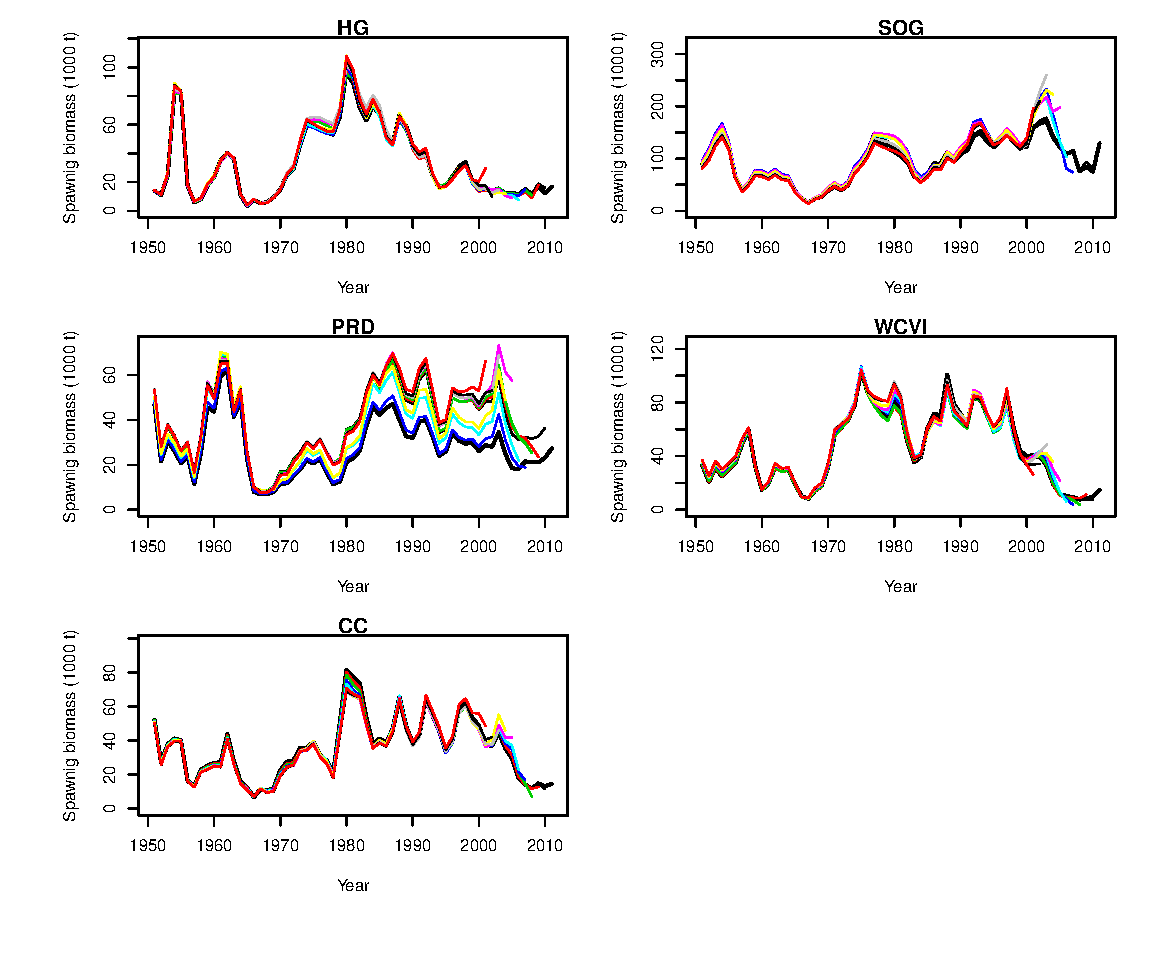
\includegraphics[scale=0.45]{../FIGS/qPriorFigs/iscam_fig_sbt_retrospective}	
		\vspace{-1cm}
		\caption{Retrospective estimates of spawning biomass.}
	\end{figure}
\end{frame}
%
\begin{frame}[t]\frametitle{Diagnostics: Trace plots}
	\begin{figure}[htbp]
		\centering
		\vspace{-0.75cm}	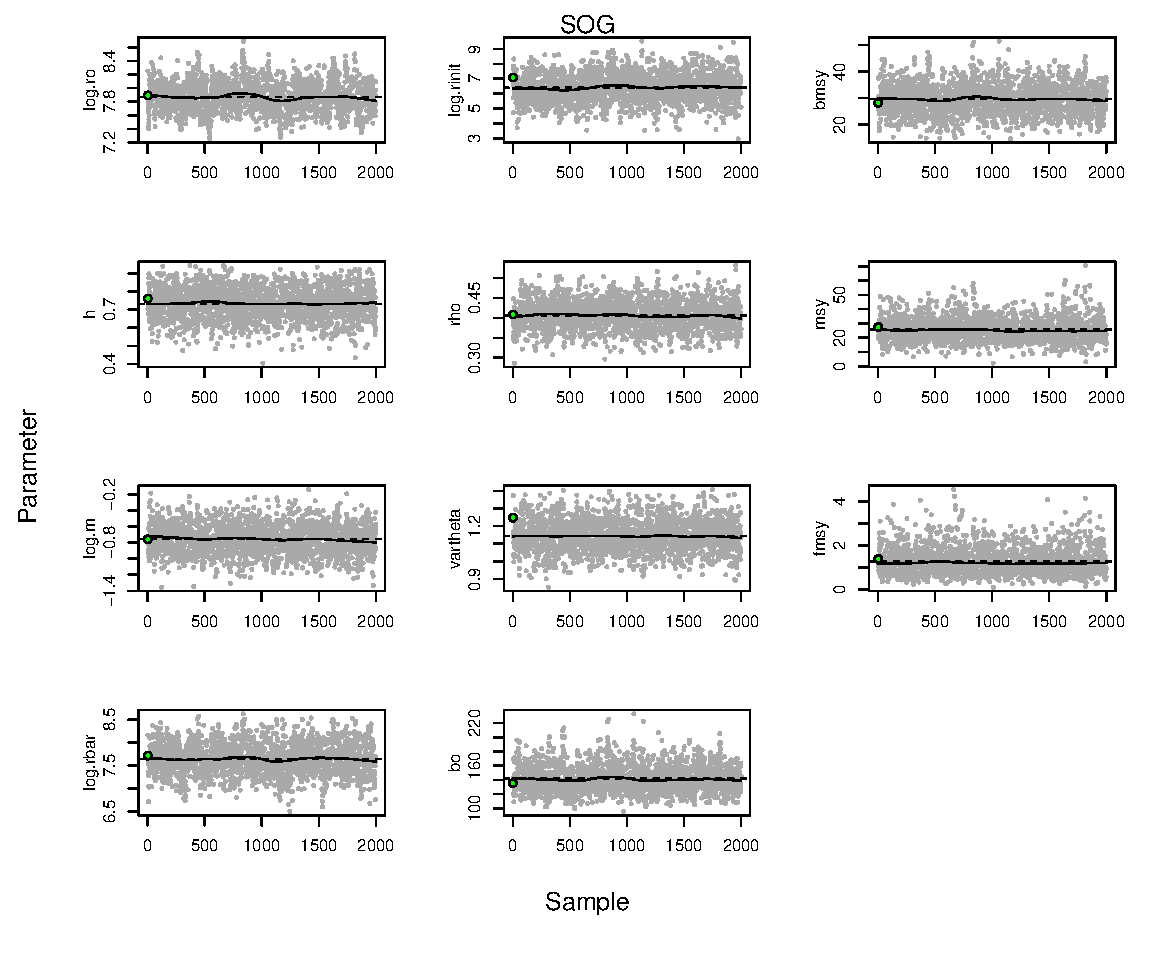
\includegraphics[scale=0.35]{../FIGS/qPriorFigs/iscam_fig_trace_SOG}
		\vspace{-0.65cm}
		\caption{Posterior samples: 1 million, thin 500, Strait of Georgia}
	\end{figure}
	
\end{frame}
%
\begin{frame}[t]\frametitle{Diagnostics: Pair plots}
	\begin{figure}[htbp]
		\centering
		\vspace{-1cm}	\includegraphics[scale=0.4]
		{../FIGS/qPriorFigs/iscam_fig_pairs_SOG}
		\vspace{-0.85cm}
		\caption{Posterior samples from leading parameters \& derived variables.}
	\end{figure}
\end{frame}
%
\begin{frame}[t]\frametitle{Diagnositcs: Marginal posteriors}
	\begin{figure}[htbp]
		\centering
			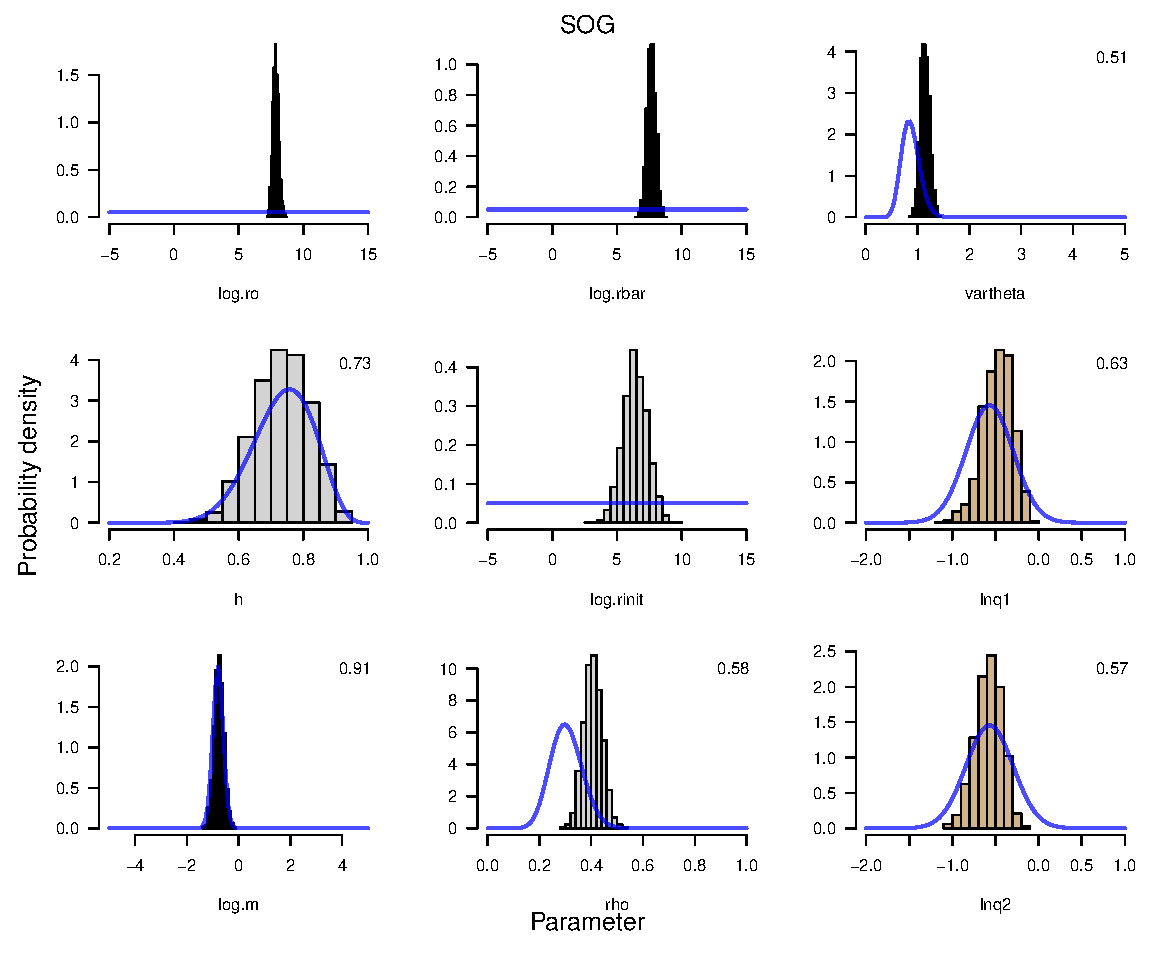
\includegraphics[scale=0.4]{../FIGS/qPriorFigs/iscam_fig_marginals_SOG}
		\caption{Strait of Georgia: Marginal \& prior distributions.}
	\end{figure}
\end{frame}
%% subsection diagnostics (end)

\subsection{Advice for management} % (fold)
\label{sub:advice_for_management}
\begin{frame}[t]\frametitle{Uncertainty in 2011 spawning biomass}
	\only<1>{
	\begin{figure}[htbp]
		\centering
			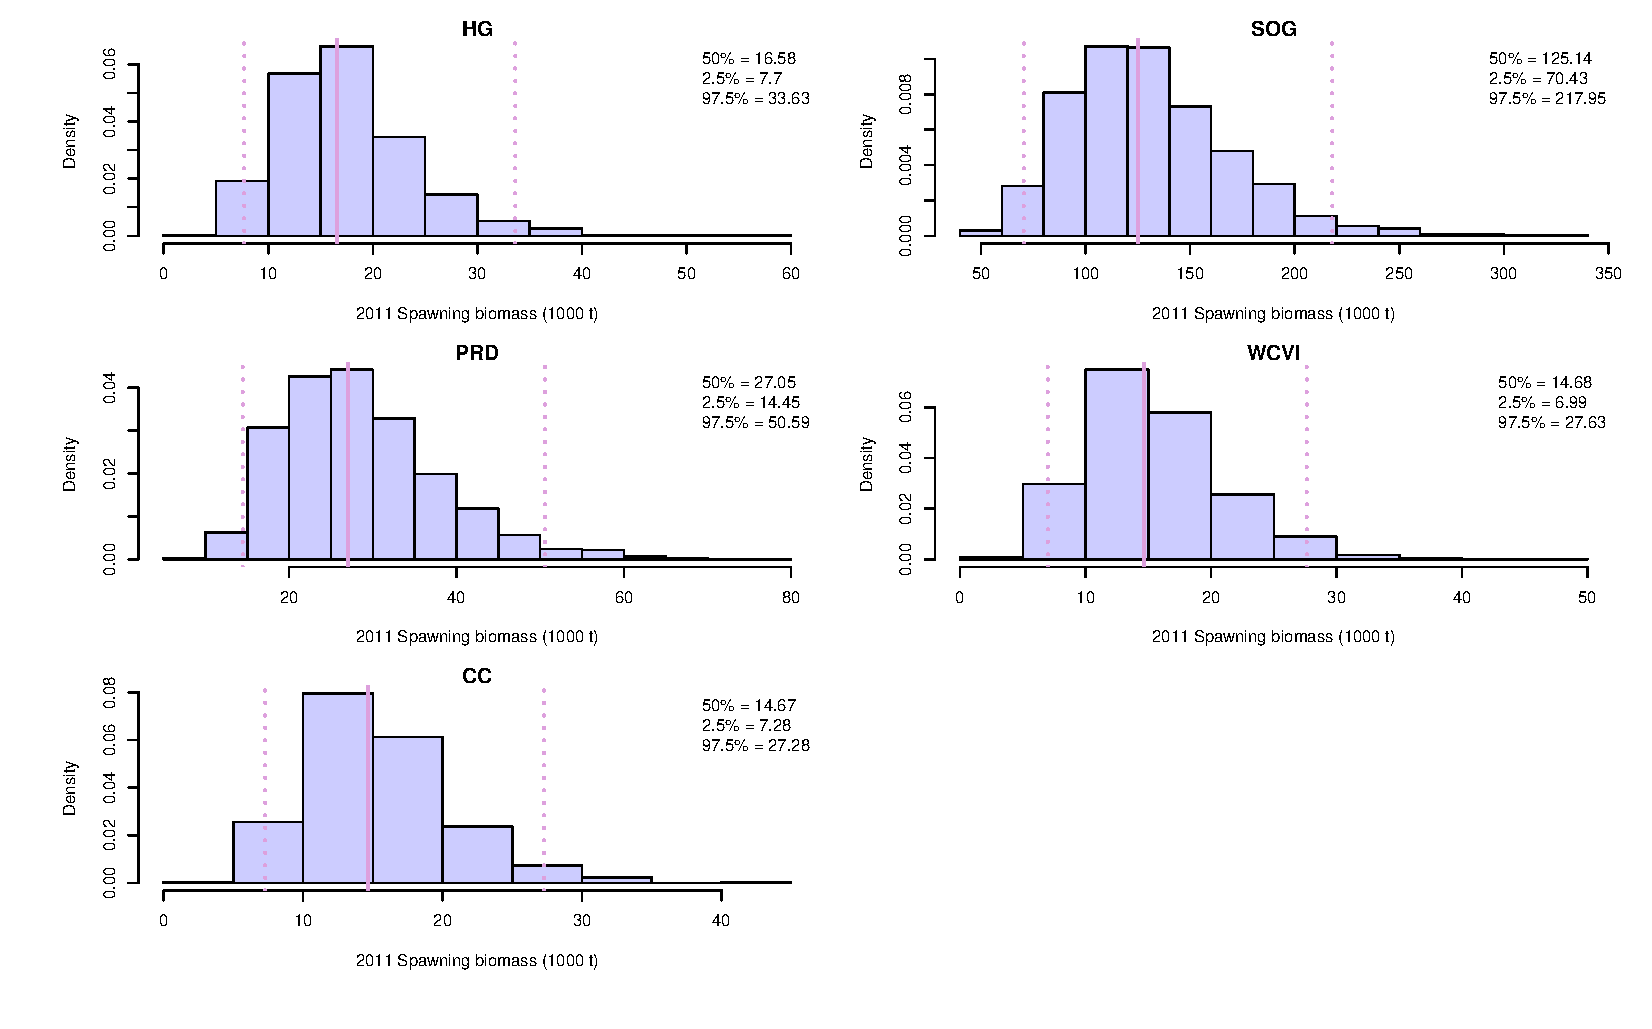
\includegraphics[scale=0.35]
			{../FIGS/qPriorFigs/iscam_fig_2011_SBt_posteriors}
		\caption{Marginal posterior distributions for 2011 spawning biomass.}
	\end{figure}
	}
	%
	\only<2>{
	\begin{figure}[htbp]
		\centering
			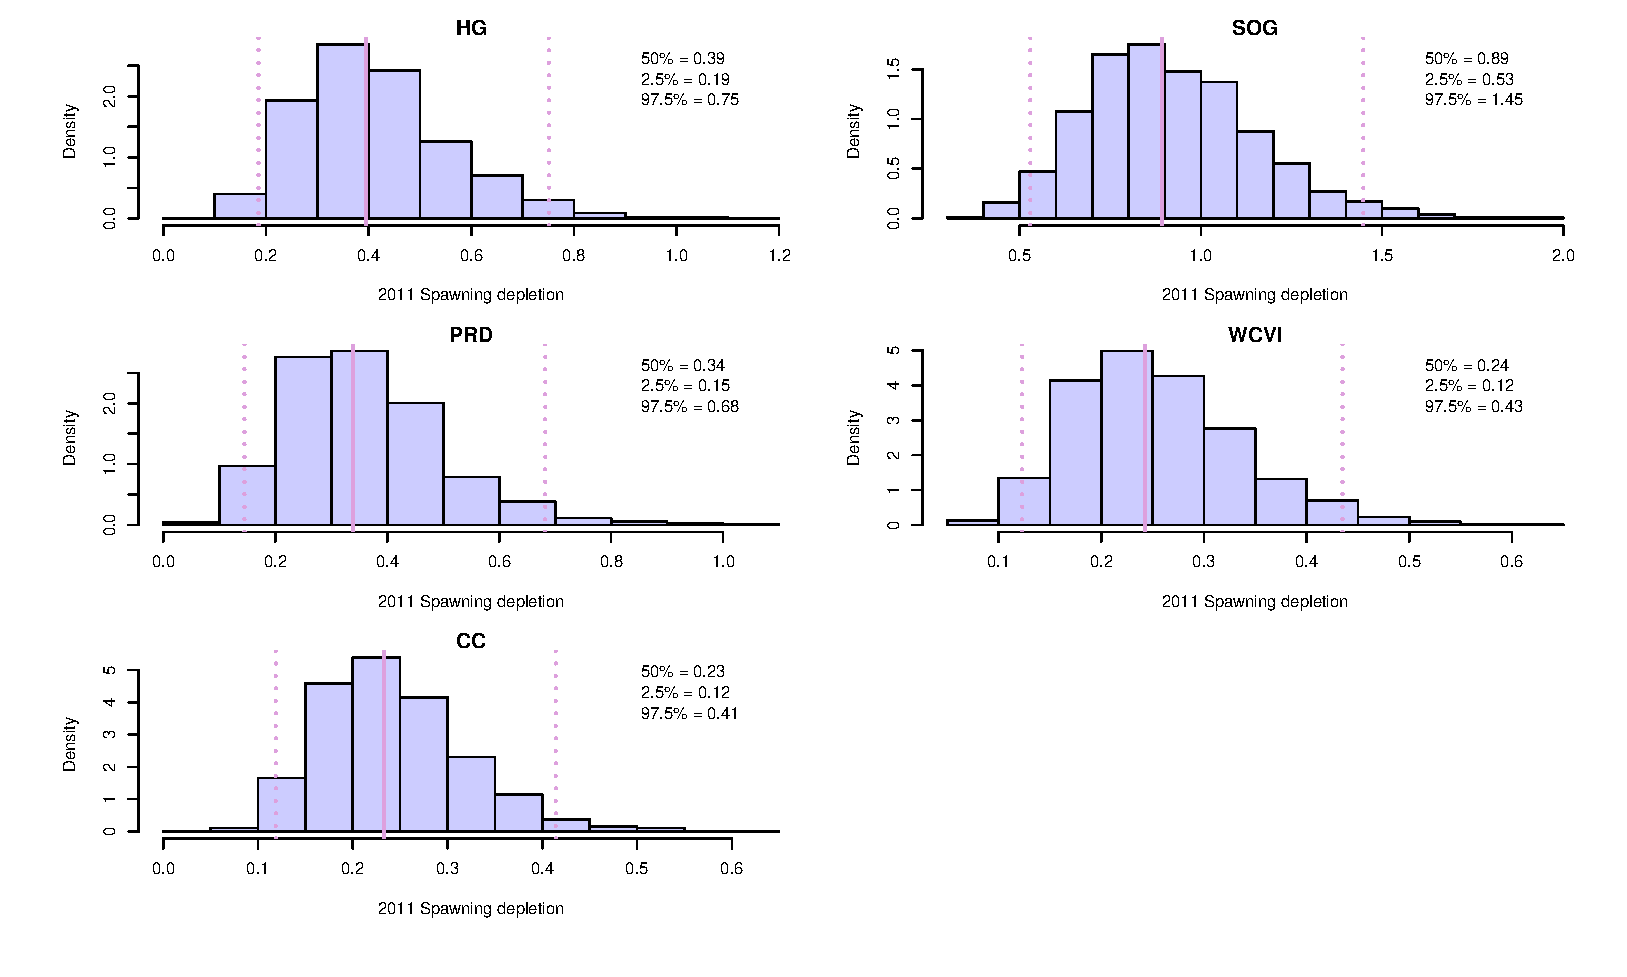
\includegraphics[scale=0.35]
			{../FIGS/qPriorFigs/iscam_fig_2011_depletion_posteriors}
		\caption{Marginal posterior distributions for 2011 spawning biomass depletion.}
	\end{figure}
	}
	%
	\only<3>{
	\begin{table}
		\caption{Estimates of 2011 spawning biomass, $B_0$, and depletion.}
		\begin{center}
		\begin{tiny}
		\begin{tabular}{l>{\bfseries}ccc|>{\bfseries}ccc|>{\bfseries}ccc}
		\hline 
		&\multicolumn{3}{c}{$SB_{2011}$} 
		&\multicolumn{3}{c}{$B_0$} 
		&\multicolumn{3}{c}{$SB_{2011}/B_0$}\\
		Stock 
		&Median & 2.5\% & 97.5\%
		&Median & 2.5\% & 97.5\%
		&Median & 2.5\% & 97.5\% \\
		\hline
		HG & 16.58 & 7.70 &33.63& 41.74 &30.05 &61.51&  0.39  &0.19  &0.75 \\
		PRD & 27.05 & 14.45&  50.59 & 78.56 & 54.15 &150.18 &  0.34  & 0.15  & 0.68\\
		CC & 14.67 & 7.28 &27.28 &62.40& 48.47& 85.06 & 0.23 & 0.12 & 0.41\\
		SOG & 125.14 & 70.43& 217.95 &140.05& 110.47& 184.24 &  0.89 &  0.53 &  1.45\\
		WCVI & 14.68 & 6.99 &27.63& 59.58& 46.84& 78.53&  0.24 & 0.12&  0.43\\
		\hline
		\end{tabular}
		\end{tiny}
		\end{center}
	\end{table}
	}
\end{frame}
%
\begin{frame}[t,shrink=35]\frametitle{Forecast: Old cutoffs}
	% latex.default(xTable, file = fn, rowname = NULL, longtable = FALSE,      landscape = FALSE, cgroup = cgrp, n.cgroup = ncgrp, caption = cap,      label = "TableCatchAdvice", na.blank = TRUE, vbar = FALSE,      size = "small") 
%
\begin{table}[!tbp]
 \small
 \caption{Estimated spawning stock biomass,  age-4+ biomass and pre-fishery
			biomass for poor average and good recruitment, old cutoffs,  and 
			available harvest based on median values from the joint posterior distribution.\label{TableCatchAdviceOldCuttoffs}} 
 \begin{center}
 \begin{tabular}{lllclllclclll}\hline\hline
\multicolumn{3}{c}{\bfseries }&
\multicolumn{1}{c}{\bfseries }&
\multicolumn{3}{c}{\bfseries Pre-fishery forecast biomass}&
\multicolumn{1}{c}{\bfseries }&
\multicolumn{1}{c}{\bfseries }&
\multicolumn{1}{c}{\bfseries }&
\multicolumn{3}{c}{\bfseries Available harvest}
\tabularnewline \cline{1-13}
\multicolumn{1}{c}{Stock}&\multicolumn{1}{c}{SSB}&\multicolumn{1}{c}{4+ Biomass}&\multicolumn{1}{c}{}&\multicolumn{1}{c}{Poor}&\multicolumn{1}{c}{Average}&\multicolumn{1}{c}{Good}&\multicolumn{1}{c}{}&\multicolumn{1}{c}{Cutoff}&\multicolumn{1}{c}{}&\multicolumn{1}{c}{Poor}&\multicolumn{1}{c}{Average}&\multicolumn{1}{c}{Good}\tabularnewline
\hline
HG&16,579& 7,089&& 9,618&12,892&21,478&&10,700&&     0& 2,192& 4,296\tabularnewline
PRD&27,046&20,593&&24,150&27,492&37,286&&12,100&& 4,830& 5,498& 7,457\tabularnewline
CC&14,666& 7,809&&11,357&14,709&22,883&&17,600&&     0&     0& 4,577\tabularnewline
SOG&125,261& 72,937&& 94,703&112,856&138,448&& 21,200&& 18,941& 22,571& 27,690\tabularnewline
WCVI&14,679& 8,267&&15,321&20,906&31,130&&18,800&&     0& 2,106& 6,226\tabularnewline
\hline
\end{tabular}

\end{center}

\end{table}


\end{frame}
%
\begin{frame}[t,shrink=35]\frametitle{Forecast: New cutoffs}
	% latex.default(xTable, file = fn, rowname = NULL, longtable = FALSE,      landscape = FALSE, cgroup = cgrp, n.cgroup = ncgrp, caption = cap,      label = "TableCatchAdvice", na.blank = TRUE, vbar = FALSE,      size = "small") 
%
\begin{table}[!tbp]
 \small
 \caption{Estimated spawning stock biomass,  age-4+ biomass and pre-fishery biomass for poor average and good recruitment, new cutoffs (based on median value of 0.25\bo\ estimated within the \iscam\ model), and available harvest based on the median values from the joint posterior distribtuion.\label{TableCatchAdviceNewCuttoffs}} 
 \begin{center}
 \begin{tabular}{lllclllclclll}\hline\hline
\multicolumn{3}{c}{\bfseries }&
\multicolumn{1}{c}{\bfseries }&
\multicolumn{3}{c}{\bfseries Pre-fishery forecast biomass}&
\multicolumn{1}{c}{\bfseries }&
\multicolumn{1}{c}{\bfseries }&
\multicolumn{1}{c}{\bfseries }&
\multicolumn{3}{c}{\bfseries Available harvest}
\tabularnewline \cline{1-13}
\multicolumn{1}{c}{Stock}&\multicolumn{1}{c}{SSB}&\multicolumn{1}{c}{4+ Biomass}&\multicolumn{1}{c}{}&\multicolumn{1}{c}{Poor}&\multicolumn{1}{c}{Average}&\multicolumn{1}{c}{Good}&\multicolumn{1}{c}{}&\multicolumn{1}{c}{Cutoff}&\multicolumn{1}{c}{}&\multicolumn{1}{c}{Poor}&\multicolumn{1}{c}{Average}&\multicolumn{1}{c}{Good}\tabularnewline
\hline
HG&16,579& 7,089&& 9,618&12,892&21,478&&10,436&&     0& 2,456& 4,296\tabularnewline
PRD&27,046&20,593&&24,150&27,492&37,286&&19,641&& 4,510& 5,498& 7,457\tabularnewline
CC&14,666& 7,809&&11,357&14,709&22,883&&15,600&&     0&     0& 4,577\tabularnewline
SOG&125,261& 72,937&& 94,703&112,856&138,448&& 35,013&& 18,941& 22,571& 27,690\tabularnewline
WCVI&14,679& 8,267&&15,321&20,906&31,130&&14,894&&   427& 4,181& 6,226\tabularnewline
\hline
\end{tabular}

\end{center}

\end{table}


\end{frame}


% subsection advice_for_management (end)

\subsection{Outstanding issues} % (fold)
\label{sub:outstanding_issues}
\begin{frame}[t]\frametitle{Outstanding issues}
	\begin{itemize}
		\item<+-> Reference points (e.g., B$_0$) based on non-stationary parameters (e.g., $M_t$, selectivity, growth).
		\item<+-> Strong retrospective bias in PRD.
		\item<+-> Formal evaluation of alternative hypotheses.
	\end{itemize}
\end{frame}

% subsection outstanding_issues (end)

\subsection{Response to reviewers} % (fold)
\label{sub:response_to_reviewers}
\begin{frame}[t]\frametitle{Risk based decision making}
	\begin{block}{Considerations}
		\begin{itemize}
			\item What is the probability of the stock falling below the cutoff for a given catch option?
			\item What is the probability of the spawning stock declining?
			\item What is the probability of the harvest rate exceeding 0.2?
		\end{itemize}
	\end{block}
\end{frame}
%
\begin{frame}[t]\frametitle{Probability of something bad happening}
	\only<1>{
	\begin{figure}[htbp]
		\centering
			\includegraphics[height=0.8\textheight]
			{../FIGS/qPriorFigs/iscam_fig_risk_HG}
			\vspace{-0.5cm}
		\caption{Haida Gwaii}
	\end{figure}
	}
	%
	\only<2>{
	\begin{figure}[htbp]
		\centering
			\includegraphics[height=0.8\textheight]
			{../FIGS/qPriorFigs/iscam_fig_risk_PRD}
			\vspace{-0.5cm}
		\caption{Prince Rupert District}
	\end{figure}
	}
	%
	\only<3>{
	\begin{figure}[htbp]
		\centering
			\includegraphics[height=0.8\textheight]
			{../FIGS/qPriorFigs/iscam_fig_risk_CC}
			\vspace{-0.5cm}
		\caption{Central Coast}
	\end{figure}
	}
	%
	\only<4>{
	\begin{figure}[htbp]
		\centering
			\includegraphics[height=0.8\textheight]
			{../FIGS/qPriorFigs/iscam_fig_risk_SOG}
			\vspace{-0.5cm}
		\caption{Strait of Georgia}
	\end{figure}
	}
	%
	\only<5>{
	\begin{figure}[htbp]
		\centering
			\includegraphics[height=0.8\textheight]
			{../FIGS/qPriorFigs/iscam_fig_risk_WCVI}
			\vspace{-0.5cm}
		\caption{West Coast Vancouver Island}
	\end{figure}
	}
\end{frame}

% subsection response_to_reviewers (end)
% section part_ii (end)


% References
\begin{frame}[t]\frametitle{Bibliography}
	\def\newblock{\hskip .11em plus .33em minus .07em}
	\bibliographystyle{apalike}
	\bibliography{$HOME/Documents/ARTICLES/Articles-1}	
\end{frame}
%



% End of slides
\end{document}